\documentclass{article}%tạo một bản báo cáo
\usepackage[utf8]{inputenc}
\usepackage[T5]{fontenc} % để sử dụng tiếng việt
\usepackage[fontsize=13pt]{scrextend} % set fontsize =13pt
\usepackage[paperheight=29.7cm,paperwidth=21cm,right=2cm,left=3cm,top=2cm,bottom=2.5cm]{geometry} % chuẩn A4, căn lề trái phải trên dưới
\usepackage{mathptmx} %timenewRoman
\usepackage{graphicx} % thư viện chèn ảnh 
\usepackage{float} % set vị trí chèn ảnh 
\usepackage{tikz} % thư viện tạo khung bìa
\usepackage{enumerate}
\usetikzlibrary{calc} % thư viện tikz
\usepackage{indentfirst} % thư viện thụt đầu dòng
\renewcommand{\baselinestretch}{1.2} % giãn dòng 1.2
\setlength{\parskip}{6pt} % giãn dòng giữa các đoạn văn(spacing after)
\setlength{\parindent}{1cm} % set khoảng cách thụt đầu dòng mỗi đoạn
\usepackage{titlesec} % thư viện để set up các kiểu  chữ
\setcounter{secnumdepth}{4}
\titlespacing*{\section}{0pt}{0pt}{30pt} % Heading 1
\titleformat*{\section}{\fontsize{16pt}{0pt}\selectfont \bfseries \centering}

\titlespacing*{\subsection}{0pt}{10pt}{0pt} % Heading 2
\titleformat*{\subsection}{\fontsize{14pt}{0pt}\selectfont \bfseries}

\titlespacing*{\subsection}{0pt}{10pt}{0pt} % Heading 3
\titleformat*{\subsection}{\fontsize{13pt}{0pt}\selectfont \bfseries \itshape}

\titlespacing*{\paragraph}{0pt}{10pt}{0pt} % Heading 4
\titleformat*{\paragraph}{\fontsize{13pt}{0pt}\selectfont \itshape}

\renewcommand{\figurename}{\fontsize{12pt}{0pt}\selectfont \bfseries Hình} %hình
\renewcommand{\thefigure}{\thesection.\arabic{figure}}
\usepackage{caption}
\captionsetup[figure]{labelsep=space}

\renewcommand{\tablename}{\fontsize{12pt}{0pt}\selectfont \bfseries Bảng} %bảng
\renewcommand{\thetable}{\thesection.\arabic{table}}
\captionsetup[table]{labelsep=space}

\usepackage{tabularx}
\newcolumntype{s}{>{\hsize=.4\hsize}X}
\newcolumntype{a}{>{\hsize=1.2\hsize}X}

\renewcommand{\theequation}{\thesection.\arabic{equation}} %thay đổi đánh số phương trình mặc định

\newtheorem{theorem}{Định lý}[section]
\newtheorem{defn}[theorem]{Định nghĩa}
\newtheorem{corollary}[theorem]{Hệ quả}
\newtheorem{lemma}[theorem]{Bổ đề}

\usepackage{lipsum} %thư viện tạo chữ linh tinh

\renewcommand{\contentsname}{MỤC LỤC}
\renewcommand{\listfigurename}{DANH MỤC HÌNH VẼ}
\renewcommand{\listtablename}{DANH MỤC BẢNG BIỂU}
\renewcommand{\refname}{TÀI LIỆU THAM KHẢO}

\usepackage[unicode]{hyperref}% để nhấn vào phần trong mục lục sẽ hiện ra phần đó

\usepackage{array}
\newcolumntype{P}[1]{>{\centering\arraybackslash}p{#1}}
\newcolumntype{M}[1]{>{\centering\arraybackslash}m{#1}}
\usepackage{colortbl}

\usepackage{listings}
\usepackage{color} % tô màu cho code
\definecolor{dkgreen}{rgb}{0,0.6,0}
\definecolor{gray}{rgb}{0.5,0.5,0.5}
\definecolor{mauve}{rgb}{0.58,0,0.82}
\lstset{frame=tb,
  % language=Dart,
  aboveskip=3mm,
  belowskip=3mm,
  showstringspaces=false,
  columns=flexible,
  basicstyle={\small\ttfamily},
  numbers=none,
  numberstyle=\tiny\color{gray},
  keywordstyle=\color{blue},
  commentstyle=\color{dkgreen},
  stringstyle=\color{mauve},
  breaklines=true,
  breakatwhitespace=true,
  tabsize=3
}




\begin{document}


\begin{titlepage}
  \begin{tikzpicture}[overlay,remember picture] % tạo khung
  \draw [line width=3pt]
       ($ (current page.north west) + (3.0cm,-2.0cm) $)
       rectangle
       ($ (current page.south east) + (-2.0cm,2.5cm) $);
      
  \draw [line width=0.5pt]
       ($ (current page.north west) + (3.1cm,-2.1cm) $)
       rectangle
       ($ (current page.south east) + (-2.1cm,2.6cm) $);
  \end{tikzpicture}
  \begin{center}
  \vspace{-12pt} ĐẠI HỌC BÁCH KHOA HÀ NỘI \\ % DẤU \\ là xuống dòng
  \textbf{\fontsize{16pt}{0pt}\selectfont TRƯỜNG ĐIỆN - ĐIỆN TỬ}
  \begin{figure}[H] % H để set vị trị ở dưới
      \vspace{0.5cm} %cách dòng trên 0.5cm
      \centering
      
\includegraphics[width=1.53cm,height=2.26cm]{Images/logohust.png}
  \end{figure}
  \vspace{1.5cm}
  \fontsize{24pt}{0pt}\selectfont ĐỒ ÁN \\ %THAY ĐỔI FONTSIZE VÀ XUỐNG DÒNG
  \vspace{12pt}
  \textbf{\fontsize{32pt}{0pt}\selectfont TỐT NGHIỆP ĐẠI HỌC} % IN ĐẬM THAY ĐỔI FONTSIZE
  \vspace{1.5cm}
  \end{center}
  \hspace{8pt}\textbf{\fontsize{14pt}{0pt}\selectfont Đề tài:}
  \begin{center}
       \textbf{\fontsize{20pt}{0pt}\selectfont XÂY DỰNG HỆ THỐNG THEO DÕI VÀ } \\
       \textbf{\fontsize{20pt}{0pt}\selectfont QUẢN LÝ DỮ LIỆU ĐIỆN TIM }
  
  \vspace{1.5cm}
  
  \begin{table}[H]%tạo bảng
       \centering
       \begin{tabular}{l l}
            \fontsize{14pt}{0pt}\selectfont Sinh viên thực hiện:      & \fontsize{14pt}{0pt}\selectfont Hoàng Anh Tuấn - 20182856\\
              &\fontsize{14pt}{0pt}\selectfont Lớp Điện tử 03 - K63  \vspace{6pt} \\
              &\fontsize{14pt}{0pt}\selectfont Đồng Minh Thái - 20193098  \\
              &\fontsize{14pt}{0pt}\selectfont Lớp Điện tử 03 - K64 \vspace{6pt} \\
            \fontsize{14pt}{0pt}\selectfont Giảng viên hướng dẫn: & \fontsize{14pt}{0pt}\selectfont TS. Nguyễn Thị Kim Thoa \\   
              &\fontsize{14pt}{0pt}\selectfont TS. Hàn Huy Dũng \vspace{6pt} \\
       \end{tabular}
  \end{table}
  \vspace{1.3cm} %3
  \fontsize{14pt}{0pt}\selectfont Hà Nội 08/2023
  \end{center}
  \end{titlepage}
  
  \cleardoublepage
  \thispagestyle{empty} %trang này không đánh số
  \begin{tikzpicture}[overlay,remember picture]
  \draw [line width=3pt]
       ($ (current page.north west) + (3.0cm,-2.0cm) $)
       rectangle
       ($ (current page.south east) + (-2.0cm,2.5cm) $);
  
  \draw [line width=0.5pt]
       ($ (current page.north west) + (3.1cm,-2.1cm) $)
       rectangle
       ($ (current page.south east) + (-2.1cm,2.6cm) $);
  \end{tikzpicture}
  \begin{center}
  \vspace{-12pt} ĐẠI HỌC BÁCH KHOA HÀ NỘI \\ % DẤU \\ là xuống dòng
  \textbf{\fontsize{16pt}{0pt}\selectfont TRƯỜNG ĐIỆN - ĐIỆN TỬ}
  \begin{figure}[H] % H để set vị trị ở dưới
  \vspace{0.5cm} %cách dòng trên 0.5cm
  \centering
  
\includegraphics[width=1.53cm,height=2.26cm]{Images/logohust.png}
  \end{figure}
  \vspace{1.5cm}
  \fontsize{24pt}{0pt}\selectfont ĐỒ ÁN \\ %THAY ĐỔI FONTSIZE VÀ XUỐNG DÒNG
  \vspace{12pt}
  \textbf{\fontsize{32pt}{0pt}\selectfont TỐT NGHIỆP ĐẠI HỌC} % IN ĐẬM THAY ĐỔI FONTSIZE
  \vspace{1.5cm}
  \end{center}
  \hspace{8pt}\textbf{\fontsize{14pt}{0pt}\selectfont Đề tài:}
  \begin{center}
     \textbf{\fontsize{20pt}{0pt}\selectfont XÂY DỰNG HỆ THỐNG THEO DÕI VÀ } \\
     \textbf{\fontsize{20pt}{0pt}\selectfont QUẢN LÝ DỮ LIỆU ĐIỆN TIM }
  
  \vspace{1.5cm}
  %tạo bảng
  \begin{table}[H]
       \centering
       \begin{tabular}{l l}
            % \fontsize{14pt}{0pt}\selectfont Sinh viên thực hiện:      & \fontsize{14pt}{0pt}\selectfont Hoàng Anh Tuấn \\
            % &\fontsize{14pt}{0pt}\selectfont Lớp Điện tử 03 - K63 \vspace{6pt} \\
            % &\fontsize{14pt}{0pt}\selectfont Đồng Minh Thái - 20193098  \\
            % &\fontsize{14pt}{0pt}\selectfont Lớp Điện tử 03 - K64 \vspace{6pt} \\
            \fontsize{14pt}{0pt}\selectfont Sinh viên thực hiện:      & \fontsize{14pt}{0pt}\selectfont Đồng Minh Thái - 20193098 \\
            &\fontsize{14pt}{0pt}\selectfont Lớp Điện tử 03 - K64 \vspace{6pt} \\
            &\fontsize{14pt}{0pt}\selectfont Hoàng Anh Tuấn - 20182856  \\
            &\fontsize{14pt}{0pt}\selectfont Lớp Điện tử 03 - K63 \vspace{6pt} \\
            \fontsize{14pt}{0pt}\selectfont Giảng viên hướng dẫn: & \fontsize{14pt}{0pt}\selectfont TS. Nguyễn Thị Kim Thoa  \vspace{6pt} \\  
              &\fontsize{14pt}{0pt}\selectfont TS. Hàn Huy Dũng \vspace{6pt} \\
            \fontsize{14pt}{0pt}\selectfont Cán bộ phản biện : &
       \end{tabular}
  \end{table}
  \vspace{0.4cm} %3
  \fontsize{14pt}{0pt}\selectfont Hà Nội 08-2023
  \end{center}
  
  \cleardoublepage %sang tờ mới
  
\section*{LỜI NÓI ĐẦU} % dấu * để không đánh sô thứ tự vào lời nói đầu
\thispagestyle{empty}
Phần này trình bày một cách rất khái quát (khoảng 1 đến 2 trang) với bối cảnh hình thành và mục đích đồ án. 
Lời cảm ơn với những tổ chức và cá nhân góp phần trong việc hoàn thiện đồ án(nếu có) nên đặt cuối mục này

\cleardoublepage

\section*{LỜI CAM ĐOAN} % dấu * để không đánh sô thứ tự vào lời nói đầu
\thispagestyle{empty}

Chúng em gồm Hoàng Anh Tuấn, mã số sinh viên 20182856, sinh viên lớp Điện tử 03, khóa K63 và Đồng Minh Thái, mã số sinh viên 20193098, sinh viên lớp Điện tử 03, khóa K64.

Chúng em xin cam đoan toàn bộ nội dung được trình bày trong đồ án Xây dựng hệ thống theo dõi và quản lý dữ liệu điện tim là kết quả quá trình tìm hiểu và
nghiên cứu của chúng em. Các dữ liệu được nêu trong đồ án là hoàn toàn trung thực
và chưa từng được người khác công bố. Mọi thông tin trích dẫn đều tuân thủ các quy
định về sở hữu trí tuệ; các tài liệu tham khảo được liệt kê rõ ràng. Chúng em xin
chịu hoàn toàn trách nhiệm với những nội dung được viết trong đồ án này.


\vspace{6pt}

\hspace{8cm}Hà Nội, ngày 10 tháng 08 năm 2023

\hspace{9cm}\textbf{Người cam đoan}

\vspace{1cm}
\hspace{7cm}\textbf{HOÀNG ANH TUẤN, ĐỒNG MINH THÁI}

\cleardoublepage

% %mục lục
% \phantomsection\addtocontents{toc}{\protect\thispagestyle{empty}}
% \tableofcontents % tạo mục lục tự động
% \thispagestyle{empty}
% \thispagestyle{empty}
% \cleardoublepage


\clearpage
\pagestyle{empty} % Loại bỏ số trang trên các trang trong mục lục
\phantomsection
\addtocontents{toc}{\protect\thispagestyle{empty}}
\setstretch{1.2}
\tableofcontents % tạo mục lục tự động
\clearpage
\pagestyle{plain} % Khôi phục lại kiểu số trang cho các trang sau mục lục
\thispagestyle{empty}
\thispagestyle{empty}
\cleardoublepage

\pagenumbering{roman} %đánh số thứ tự la mã
\phantomsection\section*{DANH MỤC KÝ HIỆU VÀ CHỮ VIẾT TẮT}%dấu * để không đánh số
\addcontentsline{toc}{section}{\numberline{}DANH MỤC KÝ HIỆU VÀ CHỮ VIẾT TẮT} % LƯU VÀO TRONG MỤC LỤC



\begin{table}[H]
  \centering
  \begin{tabularx}{0.85\textwidth}{
  | >{\centering\arraybackslash}m{3cm}
  | >{\centering\arraybackslash}X|
  }
  \hline
  \bfseries Từ viết tắt     &\bfseries Thay cho\hspace{1cm}\\ \hline
  API     & Application Programming Interface \\ \hline
  JWT  & JSON Web Token \\ \hline
  ECG   & Electrocardiogram \\ \hline
  HTML   & Hypertext Markup Language \\ \hline
  ID    & Identification \\ \hline
  3NF   & Third Normal Form \\ \hline
  ERD     & Entity-Relationship Diagram \\ \hline
  AWS  & Amazon Web Services \\ \hline
  RDS   & Relational Database Service \\ \hline
  EC2   & Elastic Compute Cloud \\ \hline
  FPS   & Frames Per Second \\ \hline
  IOT   & Internet Of Things \\ \hline
  UML   & Unified Modeling Language \\ \hline

  
  \end{tabularx}
  \label{bang31}
\end{table}


\cleardoublepage

{
\let\oldnumberline\numberline
\renewcommand{\numberline}{\figurename~\oldnumberline}%
\listoffigures
} %tạo danh mục hình vẽ tự động
\phantomsection\addcontentsline{toc}{section}{\numberline{}DANH MỤC KÝ HÌNH VẼ}
\cleardoublepage

{
\let\oldnumberline\numberline
\renewcommand{\numberline}{\tablename~\oldnumberline}%
\listoftables
} %tạo danh mục hình vẽ tự động %tạo danh mục bảng biểu
\phantomsection\addcontentsline{toc}{section}{\numberline{}DANH MỤC BẢNG BIỂU}
\cleardoublepage

\section*{TÓM TẮT ĐỒ ÁN}
\phantomsection\addcontentsline{toc}{section}{\numberline{}TÓM TẮT ĐỒ ÁN}

Đồ án "Xây dựng hệ thống theo dõi và quản lý dữ liệu điện tim" là hệ thống Web/App/Server, với kết nối Bluetooth
sử dụng công nghệ Bluetooth Low Energy giúp việc theo dõi dữ liệu điện tim trên ứng dụng di động một cách dễ dàng và
hiệu quả. Dữ liệu sau khi hoàn tất phiên đo được lưu trữ lên server để người dùng có thể xem lại bất kỳ lúc nào, đồng thời
dữ liệu có thể được sử dụng cho nhiều mục đích nghiên cứu sau này.

Trong đồ án này, chúng em tập trung hoàn thiện theo quy trình phát triển phần mềm, sau khi xác định được các yêu cầu của hệ thống
sẽ tiến hành phân tích, thiết kế và triển khai hệ thống. Trong quá trình phân tích và thiết kế chúng em áp dụng phương pháp
phân tích và thiết kế hướng đối tượng, đồng thời sử dụng ngôn ngữ UML để biểu diễn các luồng thực hiện hành động. Ứng dụng di
động được chúng em xây dựng trên hệ điều hành Android và IOS sử dụng Flutter Framework, ứng dụng Web chúng em sử dụng AdminJS, và server
là NodeJS. Hệ thống server được triển khai trên Amazon EC2. Cơ sở dữ liệu chúng em sử dụng là MySQL và NoSQL.

Quyển đồ án được trình bày theo quy trình phát triển phần mềm, nội dung mỗi chương được chúng em triển khai và trình bày thông qua sơ đồ và diễn giải chi tiết. 
Các chương theo thứ tự lần lượt là phân tích hệ thống, thiết kế hệ thống, triển khai và kiểm thử, cuối cùng là kết luận.

% \cleardoublepage

\newpage
\section*{ABSTRACT}
% \phantomsection\addcontentsline{toc}{section}{\numberline{}ABSTRACT}
The project "Development of a System for Monitoring and Managing Electrocardiogram Data" is a Web/App/Server system that utilizes Bluetooth connectivity through Bluetooth Low Energy technology, enabling easy and effective monitoring of ECG data on mobile applications. After completing a measurement session, the data is stored on the server, allowing users to review it at any time. Additionally, this data can be used for various future research purposes.

In this project, we focus on the software development lifecycle. After identifying the system requirements, 
we proceed with the analysis, design, and implementation phases. During the analysis and design, 
we apply the object-oriented analysis and design approach, utilizing the UML language to represent action workflows. 
We have developed the mobile application on Android and iOS operating systems using the Flutter Framework. 
The web application is built using AdminJS, while the server is powered by NodeJS. 
The server system is deployed on Amazon EC2. The databases used are MySQL and NoSQL.

The project report is structured according to the software development lifecycle. Each chapter's content is presented and elaborated using diagrams and detailed explanations. The chapters, in sequential order, cover system analysis, system design, deployment and testing, and finally, the conclusion.
\cleardoublepage





\section*{PHẦN MỞ ĐẦU}
\phantomsection\addcontentsline{toc}{section}{\numberline{} PHẦN MỞ ĐẦU}
\subsection*{Đặt vấn đề}
% \addcontentsline{toc}{section}{\numberline{} Đặt vấn đề}
% Cuộc cách mạng công nghiệp lần thứ tư (hay còn được gọi là cuộc cách mạng công nghiệp 4.0) đã và đang phát triển với tốc
% độ rất nhanh, ảnh hưởng đến mọi mặt đời sống xã hội. Nội dung cốt lõi của cuộc cách mạng chính là sự kết hợp giữa 
% khoa học công nghệ, trí tuệ nhân tạo và sự sáng tạo của con người. Đối với Việt Nam đang trong quá trình công nghiệp hoá, 
% hiện đại hoá, việc áp dụng được những công nghệ mới trong một số lĩnh vực thiết yếu của xã hội, đặc biệt trong ngành y tế, 
% chính là nền tảng quan trọng để chăm sóc sức khoẻ con người, từ đó tạo nên những con người với sức khoẻ tốt nhất, sẵn sàng 
% đóng góp cho sự phát triển của đất nước. 
Lĩnh vực y tế đang có những bước chuyển mình lớn trong cuộc cách mạng công nghiệp lần thứ tư 
(hay còn được gọi là cuộc cách mạng công nghiệp 4.0). Đại dịch COVID-19 đã chứng minh được tầm quan trọng của việc áp dụng
khoa học kỹ thuật vào những sản phẩm y tế giúp đẩy lùi dịch bệnh,
có thể kể đến như máy rửa tay tự động do TS.Hàn Huy Dũng (đang công tác tại Trường Điện - Điện tử, thuộc Đại học Bách khoa Hà Nội) 
\cite{ref_thay_dzung} cùng các cộng sự sáng chế, và một số ứng dụng di động
nổi bật được hầu hết người dân Việt Nam sử dụng trong đại dịch COVID-19 như Bluezone - ứng dụng cảnh báo tiếp xúc gần với
những người nhiễm COVID qua Bluetooth low energy, ứng dụng NCOVI, theo dõi các ca nhiễm và thực hiện khai báo y tế, ứng
dụng PC-Covid để cập nhật các thông tin tiêm vắc xin, thông tin xét nghiệm. Đây là một tín hiệu cho thấy nước ta đang áp
dụng công nghệ 4.0 vào trong ngành y tế một cách chủ động. Hiện nay, việc chăm sóc sức khoẻ đang được chú trọng, đối với 
những những người muốn tự theo dõi sức khoẻ bản thân
thì các thiết bị nhỏ gọn có chức năng hỗ trợ đo và một ứng dụng di động hỗ trợ việc theo dõi sức khoẻ là một trong những
điều quan trọng và cần thiết. Kể cả đối với những người gặp vấn đề về sức khoẻ, việc đến bệnh viện đông đúc để theo dõi
và khám là khá khó khăn. Câu hỏi đặt ra là có phương án khả thi nào có thể áp dụng cho việc chăm sóc sức khoẻ một cách cụ thể, 
người dùng vẫn có thể theo dõi sức khoẻ tại nhà, đồng thời có sự cố vấn và hỗ trợ của những người có chuyên môn không?

\subsection*{Đề xuất hệ thống}
% \phantomsection\addcontentsline{toc}{section}{\numberline{} Đề xuất hệ thống}

Trong mục Đặt vấn đề, chúng em có trình bày về vấn đề chăm sóc sức khoẻ tại nhà, ở mục này, chúng em xin phép đề xuất một hệ thống
dựa trên những tiến bộ của khoa học kĩ thuật, với nền tảng là sự kết hợp giữa thiết bị IOT cùng hệ thống ứng dụng theo dõi, lưu trữ,
giúp tiết kiệm thời gian cũng như tăng khả năng tiếp cận cho nhiều người dùng. 

Với nền tảng được tiếp cận thiết bị đo điện tim của mẹ và thai nhi bằng điện cực không tiếp xúc trong thời gian gần đây, 
cùng với đó là việc phát triển các thiết bị IOT đang rất được chú trọng hiện nay, chúng em mong muốn xây dựng được một hệ thống
có thể kết nối được các thiết bị đo điện tim, thu thập dữ liệu điện tim thời gian thực, đồng thời có thể lưu trữ và phục vụ cho mục đích
phân tích dữ liệu về sau này. Cụ thể, hệ thống chúng em đề xuất sẽ gồm:

- Một ứng dụng di động cho riêng những người dùng để có thể kết nối với thiết bị đo điện tim để theo dõi trực tiếp tình trạng sức khoẻ, đồng
thời có thể trao đổi với bác sĩ về tình trạng sau các lần đo, xem tin tức về các thông tin liên quan tới sức khoẻ

- Một ứng dụng di động cho bác sĩ để có thể xem được kết quả đo của các bệnh nhân được quản lý, trao đổi được với bệnh nhân

- Một ứng dụng web cho admin để quản lý hệ thống, đặc biệt là có phần phân công bác sĩ quản lý cho bệnh nhân

- Một server để lưu cơ sở dữ liệu liên quan đến người dùng và dữ liệu đo của người dùng, có thể phục vụ cho công tác nghiên cứu và
phân tich dữ liệu sau này.

\subsection*{Mục tiêu của đề tài}
Sau khi đã trình bày đề xuất về một hệ thống theo dõi và quản lý dữ liệu điện tim, mục tiêu chúng em muốn đạt được khi
làm đề tài này đó là:

- Nắm được cơ sở lý thuyết và cách thiết kế, ứng dụng các thiết bị trong hệ thống IOT

- Thực hiện hoàn chỉnh các ứng dụng được đề ra trong mục Đề xuất hệ thống, các ứng dụng hoạt động ổn định

- Có thể kết hợp tốt với các thiết bị phần cứng đang được hợp tác nghiên cứu

- Cung cấp tài liệu tham khảo một cách đầy đủ, trung thực.

\subsection*{Phương pháp nghiên cứu}
% //TODO: hoàn thành phần phương pháp nghiên cứu
Trong đồ án lần này, chúng em đã thực hiện kết hợp nhiều phương pháp nghiên cứu

\subsection*{Kết quả đạt được}

Trong suốt quá trình thực hiện đồ án, hai chúng em Đồng Minh Thái, Hoàng Anh Tuấn đã được tìm hiểu và nghiên cứu sâu hơn về cả phần cứng,
hệ thống IOT, cách kết nối các hệ thống với nhau. Các kết quả đạt được cho đến thời điểm hoàn thiện quyển đồ án bao gồm:

- Hoàn thành quyển đồ án với nội dung chi tiết về quá trình xây dựng và phát triển hệ thống

- Hoàn thành các sản phẩm ứng dụng đã đề ra trong mục Đề xuất hệ thống, các sản phẩm đã có sự kết nối, dữ liệu điện tim được theo dõi
thời gian thực được lưu trên server, dữ liệu có thể được phân tích và nghiên cứu sau này

- Được phát triển các kỹ năng làm việc nhóm, viết đồ án, kết hợp với team phần cứng, team firmware để các sản phẩm được hoàn thiện hơn.

\subsection*{Cấu trúc đồ án}
% \phantomsection\addcontentsline{toc}{section}{\numberline{} Cấu trúc đồ án}
- Phần mở đầu: Trình bày về mục đích của đồ án, thu thập yêu cầu, đề xuất hệ thống, phần tích tính khả thi và bố cục đồ án.

- Chương 1: Trình bày chi tiết các khâu trong phân tích hệ thống. 
Bao gồm xác định yêu cầu, thiết kế sơ đồ use case, biểu đồ hoạt động, biểu đồ tuần tự.

- Chương 2: Trình bày chi tiết khâu thiết kế cho hệ thống. Bao gồm thiết kế giao diện phần mềm, thiết kết API, thiết kế cơ sở dữ liệu
và giải pháp tối ưu hiệu nặng.

- Chương 3: Trình bày khâu triền khai và kiểm thử.

- Chương 4: Kết luận và nêu ra hướng phát triển.

\cleardoublepage

% \pagenumbering{arabic}


\section*{CHƯƠNG 1. PHÂN TÍCH HỆ THỐNG}
\setcounter{section}{1}
\setcounter{subsection}{0} %LƯU Ý MỖI LẦN THÊM CHƯƠNG MỚI CẦN THÊM CÂU NÀY ĐỂ RESET THỨ TỰ CỦA SUBSECTON VỀ 1
\setcounter{table}{0} % LƯU Ý SAU MỖI LẦN GỌI BẢNG HAY HÌNH ẢNH PHẢI THÊM CÂU NÀY ĐỂ RESET THỨ TỰ
\setcounter{figure}{0} %% LƯU Ý SAU MỖI LẦN GỌI BẢNG HAY HÌNH ẢNH PHẢI THÊM CÂU NÀY ĐỂ RESET THỨ TỰ
\addcontentsline{toc}{section}{\numberline{}CHƯƠNG 1. PHÂN TÍCH HỆ THỐNG}
Trong chương này, chúng em sẽ tiến hành phân tích hệ thống cho dự án đề tài "Hệ thống theo dõi và quản lý dữ liệu điện tim" dựa trên các mục tiêu
đã nêu ra trong Mục Đề xuất hệ thống ở Phần mở đầu. Trước tiên bài toán đặt ra ở hệ thống là:
\begin{adjustwidth}{1.5em}{}
\begin{itemize}
  \item Một ứng dụng để có thể giúp người dùng/bệnh nhân theo dõi được những thông tin cần về sức khoẻ tim mạch
  \item Trực quan và tiêu chuẩn hoá những thông tin đo được
    bằng hình ảnh hoặc số liệu để bác sĩ có thể dựa vào đó để đưa ra những đánh giá cho người dùng. Ngoài ra những thông tin này
    có thể hữu ích trong việc theo dõi sức khỏe tim mạch, theo dõi hiệu quả của liệu pháp 
    và hỗ trợ quyết định của người dùng
  \item Quản trị viên sẽ là người có thể phân công bác sĩ để chăm sóc, theo dõi sức khoẻ từ
  xa cho bệnh nhân
\end{itemize}
\end{adjustwidth}
Chi tiết về việc phân tích các yêu cầu hệ thống sẽ được chúng em trình bày ở các chương dưới.

\subsection{Yêu cầu hệ thống}
\subsubsection{Yêu cầu về người dùng hệ thống}
Hệ thống được thiết kế để phục vụ các đối tượng sau:
\begin{adjustwidth}{1.5em}{}
\begin{itemize}
    \item Bệnh nhân: Người sử dụng hệ thống để thực hiện theo dõi dữ liệu điện tim thông qua Bluetooth. Bệnh nhân có quyền truy cập vào kết quả ECG của mình, có thể được một bác sĩ phụ trách và theo dõi các thông tin liên quan đến điện tim và sức khoẻ
    \item Bác sĩ: Người sử dụng hệ thống để xem và đánh giá kết quả dữ liệu điện tim của bệnh nhân, đưa ra nhận xét và đề xuất điều trị. Bác sĩ có thể trao đổi với bệnh nhân thông qua tin nhắn và gửi thông báo quan trọng liên quan đến chăm sóc sức khỏe
    \item Quản trị viên: Người sử dụng hệ thống để quản lý các tài khoản người dùng, phân công bệnh nhân cho bác sĩ và quản lý mối quan hệ giữa bác sĩ và bệnh nhân, quản lý các bản dữ liệu đo
\end{itemize}
\end{adjustwidth}

\subsubsection{Yêu cầu chức năng}
Các chức năng chính của hệ thống bao gồm:
\begin{adjustwidth}{1.5em}{}
  \begin{itemize}
      \item Ghi lại dữ liệu điện tim: Hệ thống cho phép ghi lại tín hiệu điện tim từ máy đo ECG (Electrocardiogram) hay thiết bị đo điện tim khác với dữ liệu được truyền qua Bluetooth. Dữ liệu được chuyển tới ứng dụng của người dùng thông qua Bluetooth để lưu trữ, phân tích và có thể xem lại sau này
      \item Hiển thị và phân tích dữ liệu: Hệ thống hiển thị dữ liệu điện tim theo dạng đồ thị. Hệ thống cũng hỗ trợ xuất ra các tệp đã được chuẩn hoá cho các dữ liệu chuỗi thời gian (time-series database) để phục vụ mục đích phân tích và nghiên cứu sâu hơn
      \item Lưu trữ: Hệ thống hỗ trợ lưu dữ liệu mà người dùng đo được từ thiết bị trên cả ứng dụng và trên server của hệ thống. Dữ liệu điện tim cũng được đồng bộ hóa và lưu trữ trên máy chủ của hệ thống. Qua quá trình đồng bộ hóa, dữ liệu từ ứng dụng được truyền đến máy chủ và được lưu trữ an toàn và bảo mật trên hệ thống. Việc lưu trữ dữ liệu điện tim trên cả ứng dụng và máy chủ giúp đảm bảo rằng dữ liệu quan trọng này được lưu trữ một cách đáng tin cậy và có sẵn cho phân tích hoặc sử dụng tương lai
      \item Trao đổi và chia sẻ thông tin về dữ liệu điện tim: Hệ thống giúp người dùng có thể trao đổi trực tiếp với nhau, chia sẻ kết quả đo điện tim, hỏi đáp về các vấn đề sức khỏe hoặc thảo luận về các quyết định. Điều này mang lại sự tiện lợi và hỗ trợ đáng kể cho người dùng trong việc xác định về tình trạng sức khoẻ hiện tại của bản thân
  \end{itemize}
\end{adjustwidth}
% Hệ thống hỗ trợ các chức năng cơ bản sau đối với người dùng:
\textbf{Đối với người dùng là bệnh nhân:}
\begin{adjustwidth}{1.5em}{}
\begin{itemize}
    \item Đăng nhập và đăng ký tài khoản bằng thông tin cá nhân, bao gồm tên, địa chỉ email, ngày sinh, số điện thoại và mật khẩu
    \item Cập nhật các thông tin cá nhân
    \item Được theo dõi điện tim trực tiếp khi kết nối ứng dụng di động với thiết bị đo điện tim thông qua Bluetooth
    \item Xem kết quả ECG của mình, bao gồm biểu đồ và các thông số liên quan
    \item Theo dõi các tin tức liên quan đến sức khoẻ và tim mạch
    \item Nhận thông báo và có thể trao đổi trực tiếp với bác sĩ về tình hình sức khoẻ và các kết quả đo được từ thiết bị
\end{itemize}
\end{adjustwidth}
\textbf{Đối với người dùng là bác sĩ:}
\begin{adjustwidth}{1.5em}{}
\begin{itemize}
    \item Được cấp tài khoản để sử dụng hệ thống
    \item Cập nhật các thông tin cá nhân
    \item Xem danh sách bệnh nhân được phân công cho mình và xem kết quả ECG của từng bệnh nhân
    \item Đánh giá và đưa ra nhận xét về kết quả ECG của bệnh nhân
    \item Trao đổi các thông tin liên quan đến tình hình sức khoẻ và kết quả đo của bệnh nhân
\end{itemize}
\end{adjustwidth}
\textbf{Đối với người dùng là quản trị viên:}
\begin{adjustwidth}{1.5em}{}
\begin{itemize}
    \item Đăng nhập và đăng ký tài khoản bằng thông tin cá nhân, bao gồm tên, địa chỉ email, số điện thoại và mật khẩu
    \item Cập nhật thông tin cá nhân
    \item Quản lý danh sách người dùng trong hệ thống, bao gồm bệnh nhân và bác sĩ
    \item Phân công bệnh nhân cho các bác sĩ và quản lý mối quan hệ giữa bác sĩ và bệnh nhân
    \item Quản lý các bản ghi dữ liệu điện tim của bệnh nhân
    \item Quản lý các tin tức được đăng trên ứng dụng của người dùng
\end{itemize}
\end{adjustwidth}

\subsubsection{Yêu cầu phi chức năng}
\begin{itemize}
    \item Hệ thống hỗ trợ ngôn ngữ Tiếng Việt và Tiếng Anh
    \item Hệ thống có thể tương thích với các loại thiết bị phổ biến hiện nay (với Android: Android 10+, IOS: IOS > 12.1)
    \item Hệ thống đảm bảo tính bảo mật và quyền riêng tư thông tin của người dùng
    \item Hệ thống phải có giao diện người dùng thân thiện, dễ sử dụng để có thể tương tác mà không gặp quá nhiều khó khăn
    \item Thời gian phản hồi của hệ thống phải nhanh chóng và ổn định
    % \item Hệ thống cần sao lưu dữ liệu định kỳ để đảm bảo tính an toàn và khả năng khôi phục dữ liệu khi cần thiết.
\end{itemize}

Thông qua việc phân tích yêu cầu hệ thống, chúng ta có cái nhìn tổng quan về các chức năng, yêu cầu phi chức năng và 
các đối tượng người dùng mà hệ thống phải hỗ trợ. Phần phân tích này sẽ cung cấp cơ sở cho việc thiết kế và phát triển hệ thống quản lý ECG, 
đáp ứng đầy đủ các yêu cầu của người dùng và đảm bảo hiệu suất, bảo mật và tính khả dụng của hệ thống
% \subsection{Phân tích tổng quan hệ thống}

\subsection{Sơ đồ use case}
\subsubsection{Use case tổng quát hệ thống}
Dựa vào những phân tích về yêu cầu chức năng, các use case trong hệ thống được chúng em thể hiện ở hình dưới 
  \begin{figure}[H]
    \centering
    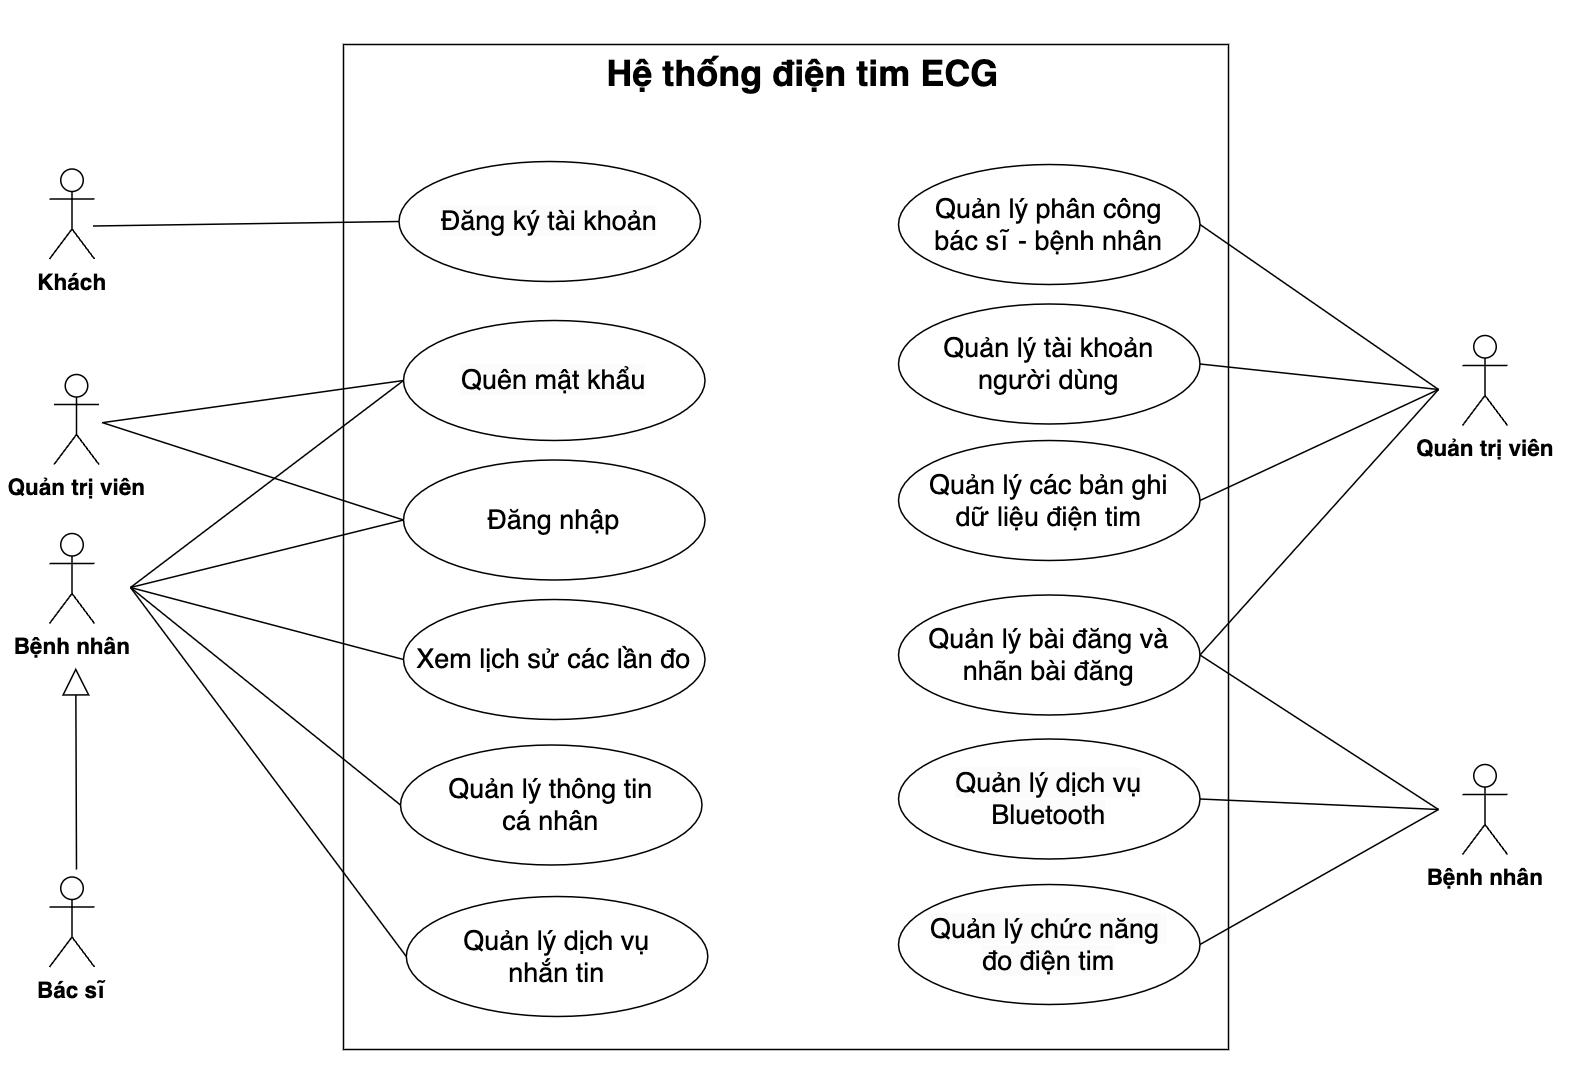
\includegraphics[width=16cm,height=14cm]{Images/use_case/use_case_general.png}
    \caption[Sơ đồ use case tổng quát của hệ thống]{\bfseries \fontsize{12pt}{0pt}
    \selectfont Sơ đồ use case tổng quát của hệ thống}
    \label{use_case_general} %đặt tên cho ảnh
  \end{figure}

\subsubsection{Use case chức năng đăng ký tài khoản}
  \begin{figure}[H]
    \centering
    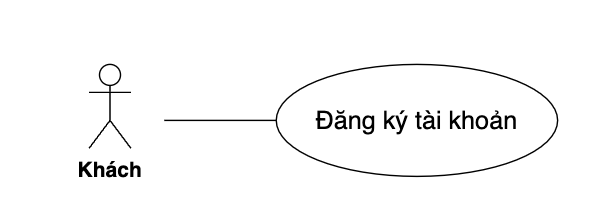
\includegraphics[width=12cm,height=4.8cm]{Images/use_case/use_case_register.png}
    \caption[Sơ đồ use case chức năng đăng ký tài khoản]{\bfseries \fontsize{12pt}{0pt}
    \selectfont Sơ đồ use case chức năng đăng ký tài khoản}
    \label{use_case_register} %đặt tên cho ảnh
  \end{figure}

  \begin{table}[H]
    \caption{\bfseries \fontsize{12pt}{0pt}\selectfont Bảng phân tích use case chức năng đăng ký}
    \centering
    \begin{tabularx}{0.9\textwidth}{|c|X|}
      \hline
      \textbf{Tên chức năng} & \textbf{Đăng ký} \\
      \hline
      Tác nhân & Khách \\
      \hline
      Mô tả & Cho phép người dùng đăng ký tài khoản để truy cập vào App/Web 
      và truy cập các tài nguyên của hệ thống \\
      \hline
      Điều kiện trước & Người dùng cần có kết nối Internet \\
      \hline
      Dòng sự kiện chính & 
      % \begin{tabular}{@{}l@{}}
        Chi tiết luồng sự kiện được thể hiện ở Hình \ref{register} và Hình \ref{backend_register}\\
      % \end{tabular} \\
      \hline
    \end{tabularx}
  \end{table}

\subsubsection{Use case chức năng quên mật khẩu}
  \begin{figure}[H]
    \centering
    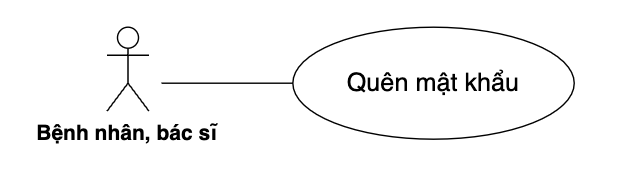
\includegraphics[width=12cm,height=4.8cm]{Images/use_case/use_case_forgot_password.png}
    \caption[Sơ đồ use case chức năng quên mật khẩu]{\bfseries \fontsize{12pt}{0pt}
    \selectfont Sơ đồ use case chức năng quên mật khẩu}
    \label{use_case_forgot_password} %đặt tên cho ảnh
  \end{figure}

  \begin{table}[H]
    \caption{\bfseries \fontsize{12pt}{0pt}\selectfont Bảng phân tích use case chức năng quên mật khẩu}
    \centering
    \begin{tabularx}{0.9\textwidth}{|c|X|}
      \hline
      \textbf{Tên chức năng} & \textbf{Quên mật khẩu} \\
      \hline
      Tác nhân & Bệnh nhân, Bác sĩ, Quản trị viên \\
      \hline
      Mô tả & Cho phép người dùng lấy lại mật khẩu bằng email khi quên mật khẩu \\
      \hline
      Điều kiện trước & Người dùng cần có kết nối Internet và truy cập được vào email đăng ký \\
      \hline
      Dòng sự kiện chính & 
      % \begin{tabular}{@{}l@{}}
        Chi tiết luồng sự kiện được thể hiện ở Hình \ref{forgot_password}, Hình \ref{resetPassword}, và Hình \ref{resetPasswordToken}\\
      % \end{tabular} \\
      \hline
    \end{tabularx}
  \end{table}

\subsubsection{Use case chức năng đăng nhập}
  \begin{figure}[H]
    \centering
    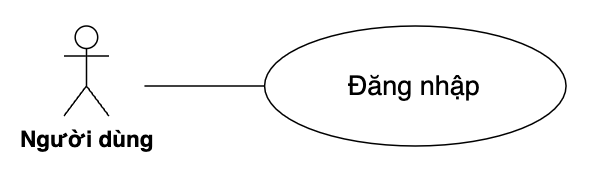
\includegraphics[width=12cm,height=4.8cm]{Images/use_case/use_case_login.png}
    \caption[Sơ đồ use case chức năng đăng nhập/đăng xuất]{\bfseries \fontsize{12pt}{0pt}
    \selectfont Sơ đồ use case chức năng đăng nhập/đăng xuất}
    \label{use_case_login} %đặt tên cho ảnh
  \end{figure}

  \begin{table}[H]
    \caption{\bfseries \fontsize{12pt}{0pt}\selectfont Bảng phân tích use case chức năng đăng nhập/đăng xuất}
    \centering
    \begin{tabularx}{0.9\textwidth}{|c|X|}
      \hline
      \textbf{Tên chức năng} & \textbf{Đăng nhập/Đăng xuất} \\
      \hline
      Tác nhân & Bệnh nhân, Bác sĩ, Quản trị viên \\
      \hline
      Mô tả & Cho phép người dùng sử dụng tài khoản để truy cập vào App/Web để truy cập các tài nguyên của hệ thống và
      có thể thoát tài khoản khỏi hệ thống\\
      \hline
      Điều kiện trước & Người dùng cần có kết nối Internet \\
      \hline
      Dòng sự kiện chính & 
      % \begin{tabular}{@{}l@{}}
        Chi tiết luồng sự kiện được thể hiện ở Hình \ref{login} và Hình \ref{backend_login}\\
      % \end{tabular} \\
      \hline
    \end{tabularx}
  \end{table}

\subsubsection{Use case chức năng xem lịch sử các lần đo}
  \begin{figure}[H]
    \centering
    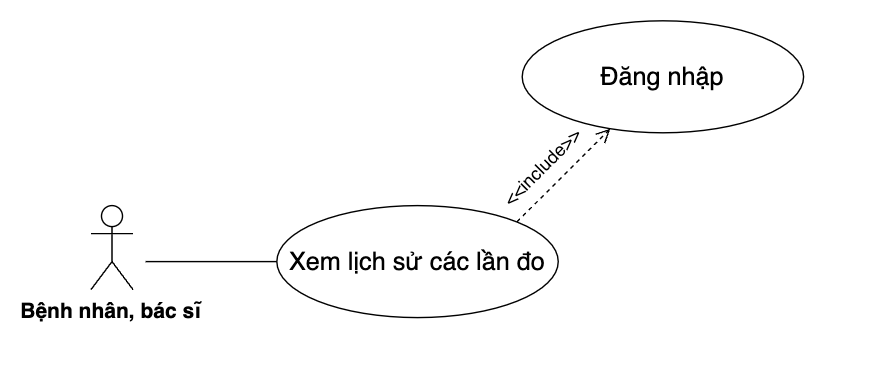
\includegraphics[width=12cm,height=4.8cm]{Images/use_case/use_case_view_history_record.png}
    \caption[Sơ đồ use case chức năng xem lịch sử các lần đo]{\bfseries \fontsize{12pt}{0pt}
    \selectfont Sơ đồ use case chức năng xem lịch sử các lần đo}
    \label{use_case_view_history_record} %đặt tên cho ảnh
  \end{figure}

  \begin{table}[H]
    \caption{\bfseries \fontsize{12pt}{0pt}\selectfont Bảng phân tích use case chức năng xem lịch sử các lần đo}
    \centering
    \begin{tabularx}{0.9\textwidth}{|c|X|}
      \hline
      \textbf{Tên chức năng} & \textbf{Xem lịch sử các lần đo} \\
      \hline
      Tác nhân & Bệnh nhân, Bác sĩ \\
      \hline
      Mô tả & Cho phép bệnh nhân xem lịch sử các lần đo điện tim và bác sĩ xem được lịch sử các lần đo của bệnh nhân
      mà mình quản lý \\
      \hline
      Điều kiện trước & Người dùng cần có kết nối Internet và đã đăng nhập \\
      \hline
      Dòng sự kiện chính & 
      % \begin{tabular}{@{}l@{}}
        Chi tiết luồng sự kiện được thể hiện ở Hình \ref{view_record_timeline}, Hình \ref{getEcgRecordsByUserId}, Hình \ref{getEcgRecordsByDoctor} 
        \\
      % \end{tabular} \\
      \hline
    \end{tabularx}
  \end{table}

\subsubsection{Use case chức năng quản lý thông tin cá nhân}
  \begin{figure}[H]
    \centering
    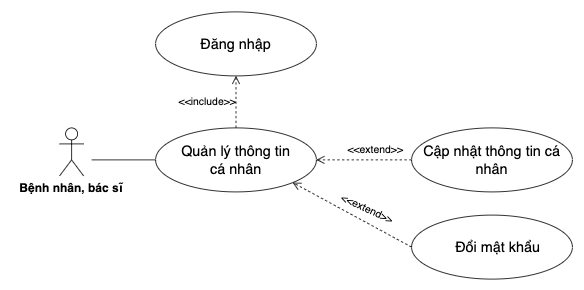
\includegraphics[width=12cm,height=4.8cm]{Images/use_case/use_case_manage_info.png}
    \caption[Sơ đồ use case chức năng quản lý thông tin cá nhân]{\bfseries \fontsize{12pt}{0pt}
    \selectfont Sơ đồ use case chức năng quản lý thông tin cá nhân}
    \label{use_case_manage_info} %đặt tên cho ảnh
  \end{figure}

  \begin{table}[H]
    \caption{\bfseries \fontsize{12pt}{0pt}\selectfont Bảng phân tích use case chức năng quản lý thông tin cá nhân}
    \centering
    \begin{tabularx}{0.9\textwidth}{|c|X|}
      \hline
      \textbf{Tên chức năng} & \textbf{Quản lý thông tin cá nhân} \\
      \hline
      Tác nhân & Bệnh nhân, Bác sĩ, Quản trị viên \\
      \hline
      Mô tả & Cho phép người dùng thay đổi thông tin cá nhân như số điện thoại, tên hiển thị, mật khẩu \\
      \hline
      Điều kiện trước & Người dùng cần có kết nối Internet và đã đăng nhập \\
      \hline
      Dòng sự kiện chính & 
      % \begin{tabular}{@{}l@{}}
        Chi tiết luồng sự kiện được thể hiện ở Hình \ref{change_user_information}, Hình \ref{change_password}, 
        Hình \ref{updateUserInfo} và Hình \ref{changePassword}
        và Hình\\
      % \end{tabular} \\
      \hline
    \end{tabularx}
  \end{table}

\subsubsection{Use case chức năng quản lý dịch vụ nhắn tin}
  \begin{figure}[H]
    \centering
    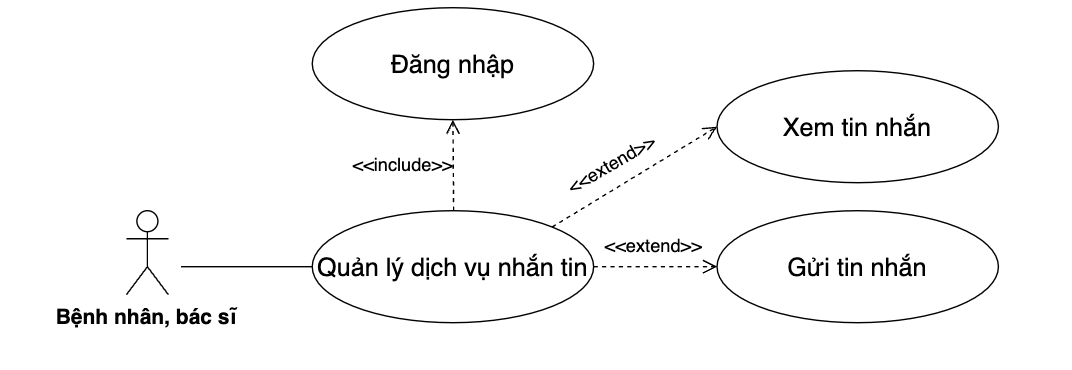
\includegraphics[width=12cm,height=4.8cm]{Images/use_case/use_case_send_receive_message.png}
    \caption[Sơ đồ use case chức năng quản lý dịch vụ nhắn tin]{\bfseries \fontsize{12pt}{0pt}
    \selectfont Sơ đồ use case chức năng quản lý dịch vụ nhắn tin}
    \label{use_case_send_receive_message} %đặt tên cho ảnh
  \end{figure}

  \begin{table}[H]
    \caption{\bfseries \fontsize{12pt}{0pt}\selectfont Bảng phân tích use case chức năng quản lý dịch vụ nhắn tin}
    \centering
    \begin{tabularx}{0.9\textwidth}{|c|X|}
      \hline
      \textbf{Tên chức năng} & \textbf{Quản lý dịch vụ nhắn tin} \\
      \hline
      Tác nhân & Bệnh nhân, Bác sĩ \\
      \hline
      Mô tả & Cho phép người dùng sử dụng tài khoản để nhắn tin trao đổi, tin nhắn sau khi được gửi sẽ được
      hiện ở dưới cùng trong khung chat \\
      \hline
      Điều kiện trước & Người dùng cần có kết nối Internet, đã đăng nhập và đã được phân công trong bảng bệnh nhân - bác sĩ \\
      \hline
      Dòng sự kiện chính & 
      % \begin{tabular}{@{}l@{}}
        Chi tiết luồng sự kiện được thể hiện ở Hình \ref{send_and_receive_message}\\
      % \end{tabular} \\
      \hline
    \end{tabularx}
  \end{table}

\subsubsection{Use case chức năng quản lý đo điện tim}
  \begin{figure}[H]
    \centering
    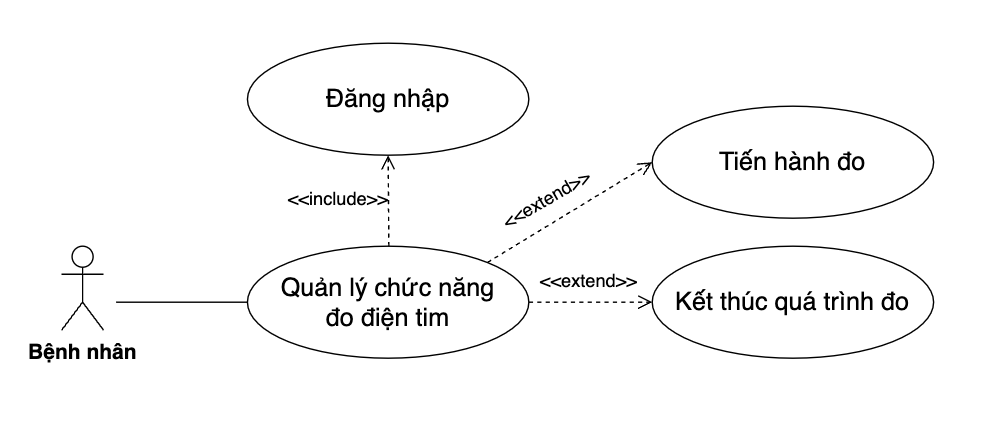
\includegraphics[width=12cm,height=4.8cm]{Images/use_case/use_case_measure_ecg.png}
    \caption[Sơ đồ use case chức năng quản lý đo điện tim]{\bfseries \fontsize{12pt}{0pt}
    \selectfont Sơ đồ use case chức năng quản lý đo điện tim}
    \label{use_case_measure_ecg} %đặt tên cho ảnh
  \end{figure}

  \begin{table}[H]
    \caption{\bfseries \fontsize{12pt}{0pt}\selectfont Bảng phân tích use case chức năng quản lý đo điện tim}
    \centering
    \begin{tabularx}{0.9\textwidth}{|c|X|}
      \hline
      \textbf{Tên chức năng} & \textbf{Quản lý đo điện tim} \\
      \hline
      Tác nhân & Bệnh nhân \\
      \hline
      Mô tả & Cho phép người dùng thực hiện thao tác bắt đầu/ kết thúc quá trình đo của mình. \\
      \hline
      Điều kiện trước & Người dùng cần bật Bluetooth và đã kết nối với thiết bị đo điện tim \\
      \hline
      Dòng sự kiện chính & 
      % \begin{tabular}{@{}l@{}}
        Chi tiết luồng sự kiện được thể hiện ở Hình \ref{start_measuring_ecg} và Hình \ref{end_measuring_ecg} \\
      % \end{tabular} \\
      \hline
    \end{tabularx}
  \end{table}

\subsubsection{Use case chức năng quản lý dịch vụ Bluetooth}
  \begin{figure}[H]
    \centering
    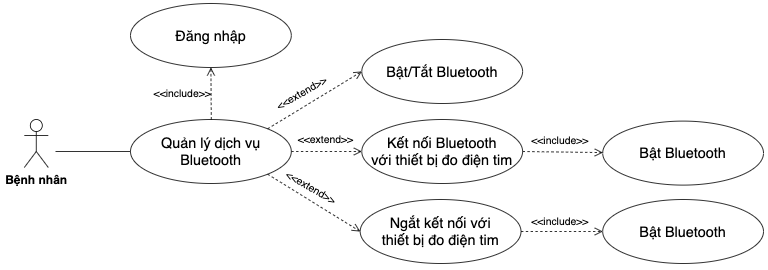
\includegraphics[width=12cm,height=4.8cm]{Images/use_case/use_case_bluetooth.png}
    \caption[Sơ đồ use case chức năng quản lý dịch vụ Bluetooth]{\bfseries \fontsize{12pt}{0pt}
    \selectfont Sơ đồ use case chức năng quản lý dịch vụ Bluetooth}
    \label{use_case_bluetooth} %đặt tên cho ảnh
  \end{figure}

  \begin{table}[H]
    \caption{\bfseries \fontsize{12pt}{0pt}\selectfont Bảng phân tích use case chức năng quản lý dịch vụ Bluetooth}
    \centering
    \begin{tabularx}{0.9\textwidth}{|c|X|}
      \hline
      \textbf{Tên chức năng} & \textbf{Quản lý dịch vụ Bluetooth} \\
      \hline
      Tác nhân & Bệnh nhân \\
      \hline
      Mô tả & Cho phép người dùng thực hiện các thao tác liên quan đến việc bật tắt và quản lý kết nối với thiết bị điện tim \\
      \hline
      Điều kiện trước & Điện thoại của người dùng có hỗ trợ Bluetooth \\
      \hline
      Dòng sự kiện chính & 
      % \begin{tabular}{@{}l@{}}
        Chi tiết luồng sự kiện được thể hiện ở Hình \ref{turn_on_off_bluetooth} \\
      % \end{tabular} \\
      \hline
    \end{tabularx}
  \end{table}

\subsubsection{Use case chức năng quản lý bài đăng và nhãn bài đăng}
  \begin{figure}[H]
    \centering
    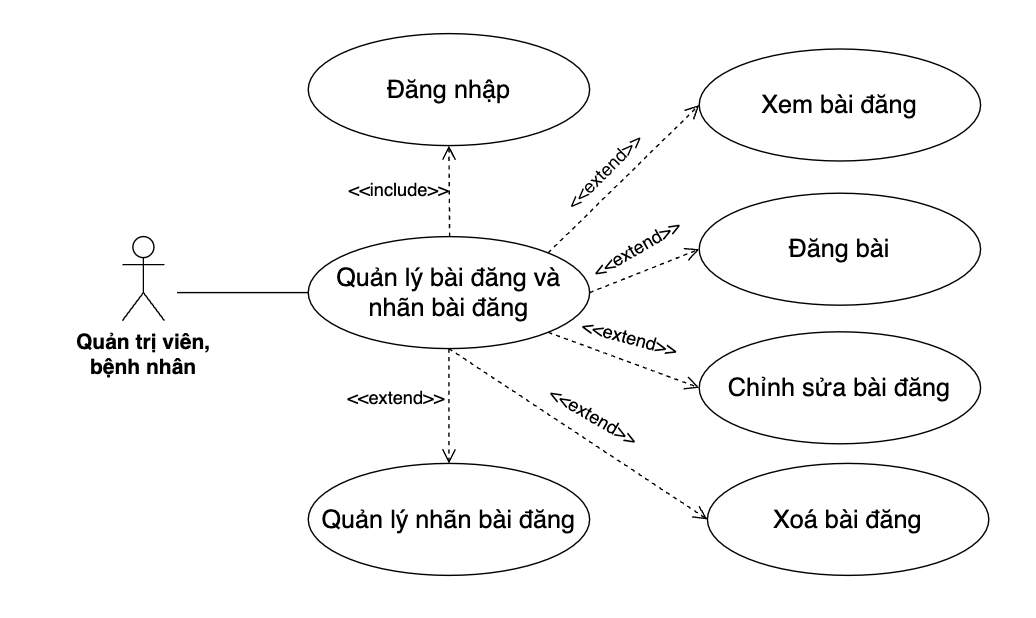
\includegraphics[width=15cm,height=8cm]{Images/use_case/use_case_news.png}
    \caption[Sơ đồ use case chức năng quản lý bài đăng]{\bfseries \fontsize{12pt}{0pt}
    \selectfont Sơ đồ use case chức năng quản lý bài đăng}
    \label{use_case_news} %đặt tên cho ảnh
  \end{figure}

  \begin{table}[H]
    \caption{\bfseries \fontsize{12pt}{0pt}\selectfont Bảng phân tích use case chức năng quản lý bài đăng và nhãn bài đăng}
    \centering
    \begin{tabularx}{0.9\textwidth}{|c|X|}
      \hline
      \textbf{Tên chức năng} & \textbf{Quản lý bài đăng và nhãn bài đăng} \\
      \hline
      Tác nhân & Bệnh nhân, Quản trị viên \\
      \hline
      Mô tả & Cho phép bệnh nhân xem các bài đăng xem các thông tin liên quan đến sức khoẻ, trong đó quản trị viên có thể
      xem, thêm, sửa, xoá các bài đăng đó  \\
      \hline
      Điều kiện trước & Người dùng cần có kết nối Internet và đã đăng nhập \\
      \hline
      Dòng sự kiện chính & 
      % \begin{tabular}{@{}l@{}}
        Chi tiết luồng sự kiện được thể hiện ở Hình \ref{view_news}, Hình \ref{getAllNews},
        và Hình \ref{getNewsById} \\
      % \end{tabular} \\
      \hline
    \end{tabularx}
  \end{table}

  \begin{figure}[H]
    \centering
    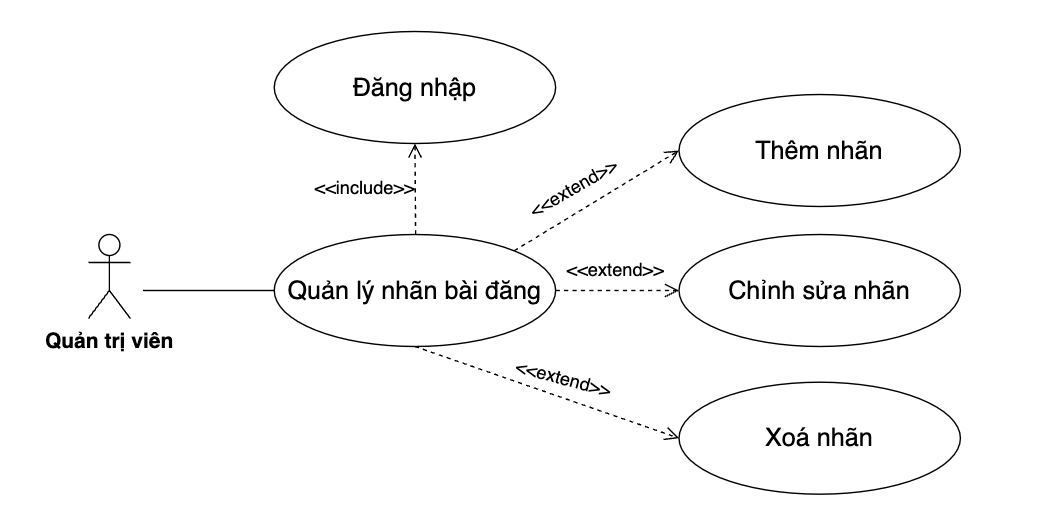
\includegraphics[width=15cm,height=7cm]{Images/use_case/use_case_category_news.png}
    \caption[Sơ đồ use case chức năng quản lý nhãn bài đăng]{\bfseries \fontsize{12pt}{0pt}
    \selectfont Sơ đồ use case chức năng quản lý nhãn bài đăng}
    \label{use_case_category_news} %đặt tên cho ảnh
  \end{figure}

  \begin{table}[H]
    \caption{\bfseries \fontsize{12pt}{0pt}\selectfont Bảng phân tích use case chức năng quản lý nhãn bài đăng}
    \centering
    \begin{tabularx}{0.9\textwidth}{|c|X|}
      \hline
      \textbf{Tên chức năng} & \textbf{Quản lý nhãn bài đăng} \\
      \hline
      Tác nhân & Quản trị viên \\
      \hline
      Mô tả & Cho phép quản trị viên thêm, sửa, xoá nhãn bài đăng và kết hợp nhãn cho từng bài đăng \\
      \hline
      Điều kiện trước & Người dùng cần có kết nối Internet và đã đăng nhập với tư cách là quản trị viên \\
      \hline
      Dòng sự kiện chính & 
      % \begin{tabular}{@{}l@{}}
        Chi tiết luồng sự kiện được thể hiện ở Hình \ref{getNewsByCategory}, Hình \ref{getAllNewsCategories}\\
      % \end{tabular} \\
      \hline
    \end{tabularx}
  \end{table}

\subsubsection{Use case chức năng quản lý các bản ghi dữ liệu điện tim}
  \begin{figure}[H]
    \centering
    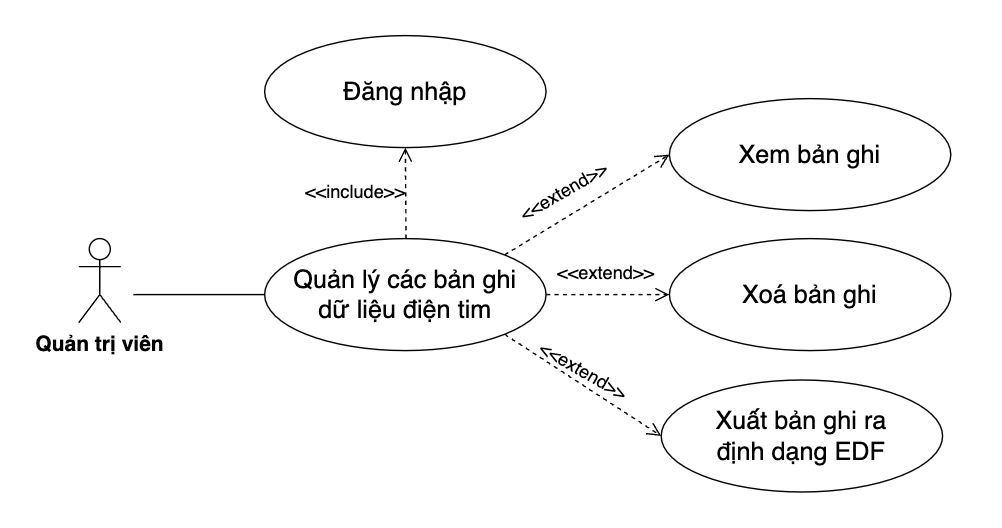
\includegraphics[width=15cm,height=7cm]{Images/use_case/use_case_manage_records.png}
    \caption[Sơ đồ use case chức năng quản lý các bản ghi dữ liệu điện tim]{\bfseries \fontsize{12pt}{0pt}
    \selectfont Sơ đồ use case chức năng quản lý các bản ghi dữ liệu điện tim}
    \label{use_case_manage_records} %đặt tên cho ảnh
  \end{figure}

  \begin{table}[H]
    \caption{\bfseries \fontsize{12pt}{0pt}\selectfont Bảng phân tích use case chức năng quản lý các bản ghi dữ liệu điện tim}
    \centering
    \begin{tabularx}{0.9\textwidth}{|c|X|}
      \hline
      \textbf{Tên chức năng} & \textbf{Quản lý các bản ghi dữ liệu điện tim} \\
      \hline
      Tác nhân & Quản trị viên \\
      \hline
      Mô tả & Cho phép quản trị viên quản lý  những bản ghi và xuất ra những định dạng phục vụ cho việc chẩn đoán của bác sĩ \\
      \hline
      Điều kiện trước & Người dùng cần có kết nối Internet và đã đăng nhập với tư cách là quản trị viên \\
      \hline
      Dòng sự kiện chính & 
      % \begin{tabular}{@{}l@{}}
        Chi tiết luồng sự kiện được thể hiện ở Hình \ref{seq_crud} mục ECGRecordsResource\\
      % \end{tabular} \\
      \hline
    \end{tabularx}
  \end{table}

\subsubsection{Use case chức năng quản lý tài khoản người dùng}
  \begin{figure}[H]
    \centering
    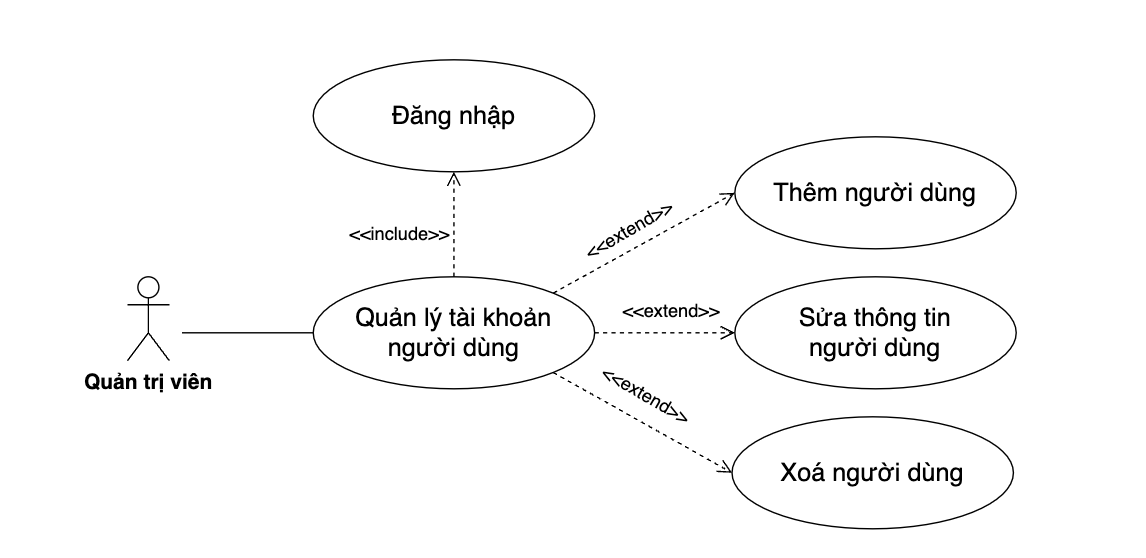
\includegraphics[width=15cm,height=7cm]{Images/use_case/use_case_manage_users.png}
    \caption[Sơ đồ use case chức năng quản lý tài khoản người dùng]{\bfseries \fontsize{12pt}{0pt}
    \selectfont Sơ đồ use case chức năng quản lý tài khoản người dùng}
    \label{use_case_manage_users} %đặt tên cho ảnh
  \end{figure}

  \begin{table}[H]
    \caption{\bfseries \fontsize{12pt}{0pt}\selectfont Bảng phân tích use case chức năng quản lý tài khoản người dùng}
    \centering
    \begin{tabularx}{0.9\textwidth}{|c|X|}
      \hline
      \textbf{Tên chức năng} & \textbf{Quản lý tài khoản người dùng} \\
      \hline
      Tác nhân & Quản trị viên \\
      \hline
      Mô tả & Cho phép quản trị viên thực hiện các hành động thêm, sửa, xoá, tìm kiến đối với tài khoản người dùng \\
      \hline
      Điều kiện trước & Người dùng cần có kết nối Internet và đã đăng nhập với tư cách là quản trị viên \\
      \hline
      Dòng sự kiện chính & 
      % \begin{tabular}{@{}l@{}}
        Chi tiết luồng sự kiện được thể hiện ở Hình \ref{seq_crud} mục DoctorResource, PatientResource và Admin Resource\\
      % \end{tabular} \\
      \hline
    \end{tabularx}
  \end{table}

\subsubsection{Use case chức năng quản lý phân công bác sĩ - bệnh nhân}
  \begin{figure}[H]
    \centering
    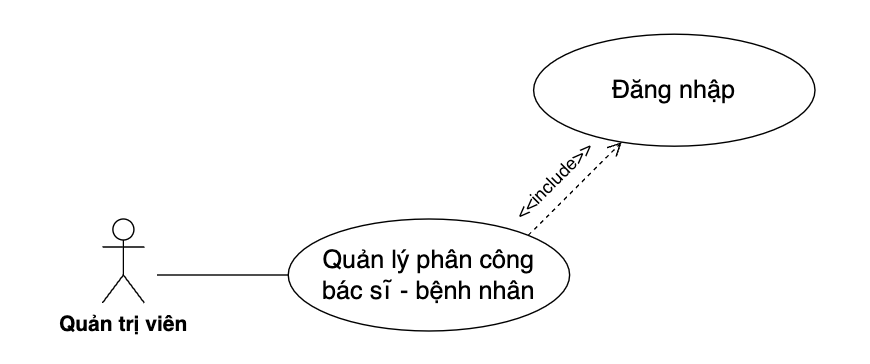
\includegraphics[width=12cm,height=4.8cm]{Images/use_case/use_case_assign_doctor.png}
    \caption[Sơ đồ use case chức năng quản lý phân công bác sĩ - bệnh nhân]{\bfseries \fontsize{12pt}{0pt}
    \selectfont Sơ đồ use case chức năng quản lý phân công bác sĩ - bệnh nhân}
    \label{use_case_assign_doctor} %đặt tên cho ảnh
  \end{figure}

  \begin{table}[H]
    \caption{\bfseries \fontsize{12pt}{0pt}\selectfont Bảng phân tích use case chức năng quản lý phân công bác sĩ - bệnh nhân}
    \centering
    \begin{tabularx}{0.9\textwidth}{|c|X|}
      \hline
      \textbf{Tên chức năng} & \textbf{Quản lý phân công bác sĩ - bệnh nhân} \\
      \hline
      Tác nhân & Quản trị viên \\
      \hline
      Mô tả & Cho phép quản trị viên phân công bác sĩ chăm sóc, theo dõi với từng bệnh nhân tương ứng để có thể xem bản ghi
      và trao đổi về sức khoẻ \\
      \hline
      Điều kiện trước & Người dùng cần có kết nối Internet và đã đăng nhập với tư cách là quản trị viên \\
      \hline
      Dòng sự kiện chính & 
      % \begin{tabular}{@{}l@{}}
        Chi tiết luồng sự kiện được thể hiện ở Hình \ref{seq_crud} mục PatientDoctorAssignmentResource\\
      % \end{tabular} \\
      \hline
    \end{tabularx}
  \end{table}

% \newpage
\subsection{Sơ đồ tuần tự}
Để phân tích cụ thể hơn từng luồng trong hệ thống qua use case, chúng em xin phép được trình bày các sơ đồ tuần
tự. 
\subsubsection{Sơ đồ tuần tự chức năng đăng ký}
  \begin{figure}[H]
        \centering
        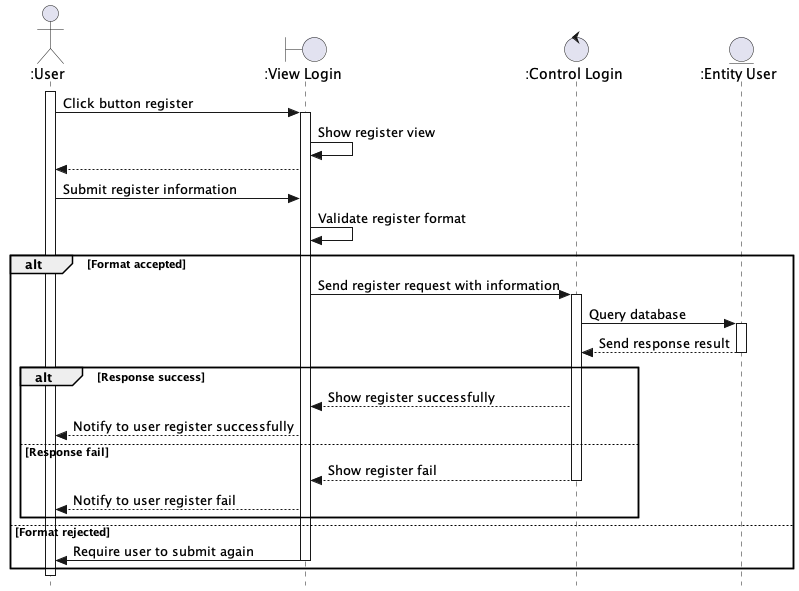
\includegraphics[width=12.9cm,height=9.4cm]{Images/mobile_app/register.png}
        \caption[Sơ đồ tuần tự chức năng đăng ký trên App]{\bfseries \fontsize{12pt}{0pt}
        \selectfont Sơ đồ tuần tự chức năng đăng ký trên App}
        \label{register} %đặt tên cho ảnh
  \end{figure}
  Sơ đồ tuần tự trên mô tả chi tiết quá trình người dùng đăng ký vào hệ thống. Người dùng gửi yêu cầu đăng ký, yêu cầu sẽ
  được xử lý bởi Control, nếu có lỗi phát sinh sẽ trả ra lỗi cho người dùng và yêu cầu người dùng nhập lại. Control
  sẽ xử lý cụ thể như thế nào được chúng em thể hiện trong Hình \ref{backend_register} trong chương sau.
\subsubsection{Sơ đồ tuần tự chức năng đăng nhập/đăng xuất}

    \begin{figure}[H]
         \centering
         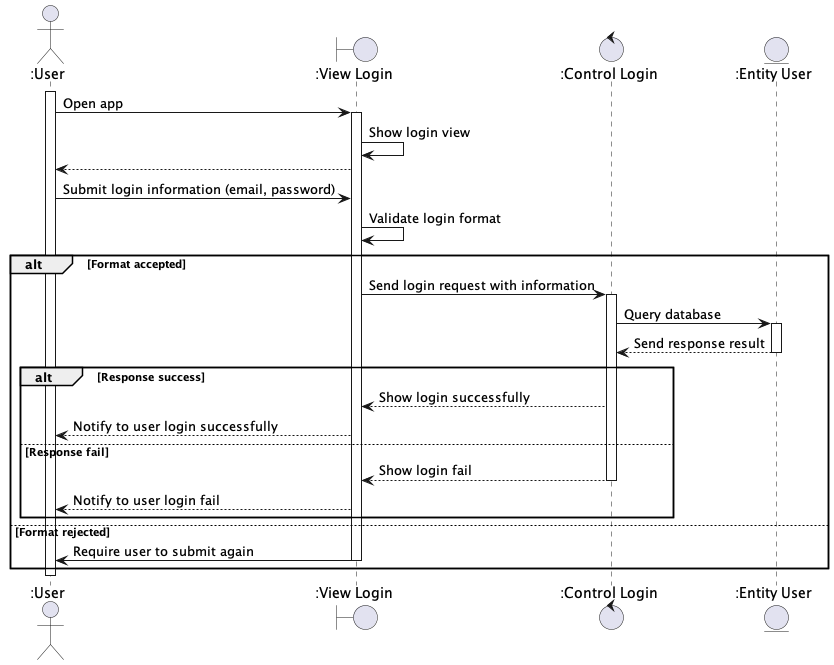
\includegraphics[width=16cm,height=12cm]{Images/mobile_app/login.png}
         \caption[Sơ đồ tuần tự chức năng đăng nhập trên App]{\bfseries \fontsize{12pt}{0pt}
         \selectfont Sơ đồ tuần tự chức năng đăng nhập trên App}
         \label{login} %đặt tên cho ảnh
    \end{figure}

  Sơ đồ tuần tự trên mô tả chi tiết quá trình người dùng đăng nhập vào hệ thống. Người dùng gửi yêu cầu đăng nhập, yêu cầu sẽ
  được xử lý bởi Control, nếu có lỗi phát sinh sẽ trả ra lỗi cho người dùng và yêu cầu người dùng nhập lại. Việc Control
  sẽ xử lý cụ thể yêu cầu người dùng được chúng em thể hiện trong Hình \ref{backend_login} trong chương sau.

  \begin{figure}[H]
    \centering
    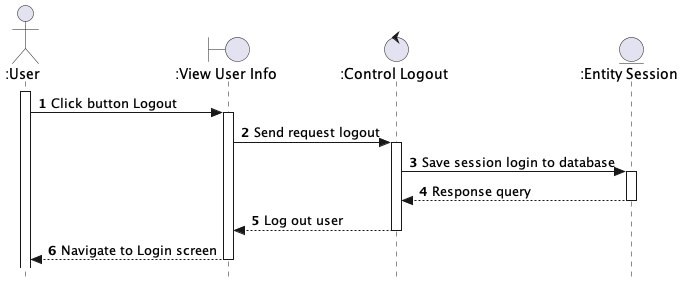
\includegraphics[width=12cm,height=6cm]{Images/mobile_app/logout.png}
    \caption[Sơ đồ tuần tự chức năng đăng xuất trên App]{\bfseries \fontsize{12pt}{0pt}
    \selectfont Sơ đồ tuần tự chức năng đăng xuất trên App}
    \label{logout} %đặt tên cho ảnh
\end{figure}

Sơ đồ tuần tự trên mô tả chi tiết quá trình người dùng đăng xuất khỏi hệ thống. Người dùng gửi yêu cầu đăng xuất, yêu cầu sẽ
được xử lý bởi Control, nếu có lỗi phát sinh sẽ trả ra lỗi cho người dùng và yêu cầu người dùng nhập lại. Việc Control
sẽ xử lý cụ thể yêu cầu người dùng được chúng em thể hiện trong Hình \ref{backend_logout} trong chương sau.


\subsubsection{Sơ đồ tuần tự chức năng quên mật khẩu}

  \begin{figure}[H]
        \centering
        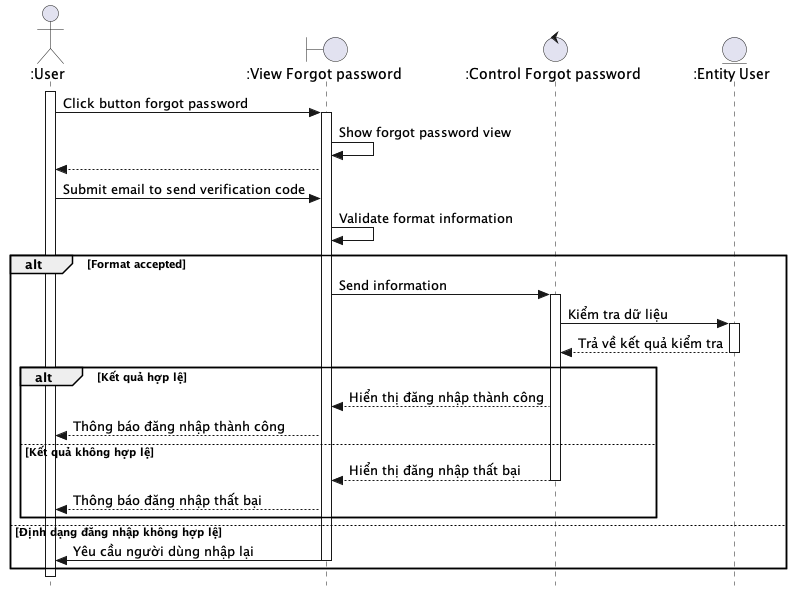
\includegraphics[width=12.9cm,height=10cm]{Images/mobile_app/forgot_password.png}
        \caption[Sơ đồ tuần tự chức năng quên mật khẩu trên App]{\bfseries \fontsize{12pt}{0pt}
        \selectfont Sơ đồ tuần tự chức năng quên mật khẩu trên App}
        \label{forgot_password} %đặt tên cho ảnh
  \end{figure}

  Sơ đồ tuần tự trên mô tả chi tiết quá trình người dùng lấy lại mật khẩu. Người dùng nhập email đã đăng ký tài khoản,
  và gửi yêu cầu lấy lại mật khẩu, Control xử lý gửi đến email một mã xác thực, người dùng nhập đúng mã xác thực sẽ được thay
  đổi mật khẩu mới. Control xử lý cụ thể yêu cầu được chúng em thể hiện trong Hình \ref{resetPassword} và Hình \ref{resetPasswordToken} trong chương sau.

\subsubsection{Sơ đồ tuần tự chức năng xem lịch sử các lần đo}

    \begin{figure}[H]
         \centering
         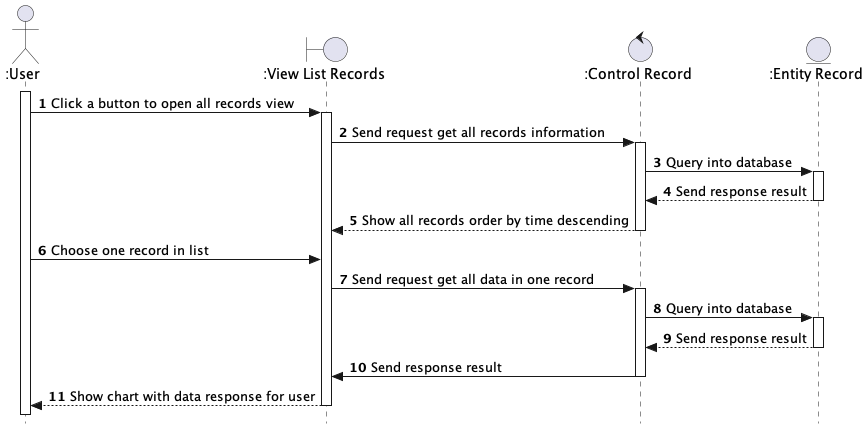
\includegraphics[width=12cm,height=6cm]{Images/mobile_app/view_record_timeline.png}
         \caption[Sơ đồ tuần tự chức năng xem lịch sử các lần đo trên App]{\bfseries \fontsize{12pt}{0pt}
         \selectfont Sơ đồ tuần tự chức năng xem lịch sử các lần đo trên App}
         \label{view_record_timeline} %đặt tên cho ảnh
    \end{figure}

    Sơ đồ tuần tự trên mô tả chi tiết quá trình người dùng xem lịch sử các lần đo. Người dùng chọn vào tab xem lịch sử, 
    lúc đó hệ thống sẽ gửi một yêu cầu lấy danh sách lịch sử các lần đo qua Control và hiển thị cho người dùng, sau đó người dùng sẽ
    chọn một bản ghi, Control sẽ lấy dữ liệu và hiển thị cho người dùng dữ liệu đo trên biểu đồ. Việc xử lý các yêu cầu cụ thể
    Hình \ref{getEcgRecordsByDoctor}, Hình \ref{convertExceltoJson} và Hình \ref{getEcgRecordsByUserId} ở chương sau.

\subsubsection{Sơ đồ tuần tự chức năng thay đổi thông tin cá nhân}

  \begin{figure}[H]
        \centering
        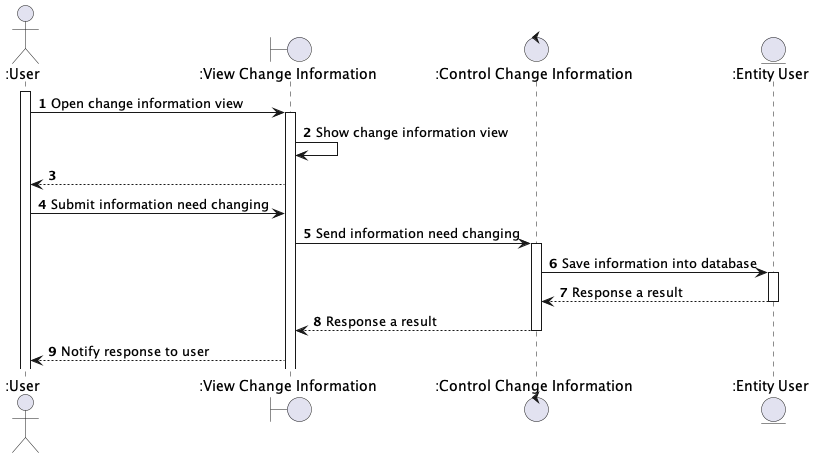
\includegraphics[width=12cm,height=6cm]{Images/mobile_app/change_user_information.png}
        \caption[Sơ đồ tuần tự chức năng thay đổi thông tin cá nhân trên App]{\bfseries \fontsize{12pt}{0pt}
        \selectfont Sơ đồ tuần tự chức năng thay đổi thông tin cá nhân trên App}
        \label{change_user_information} %đặt tên cho ảnh
  \end{figure}

  Sơ đồ tuần tự trên mô tả chi tiết quá trình người dùng thay đổi thông tin cá nhân. Người dùng thay đổi thông tin cá nhân
  và gửi yêu cầu. Control sẽ xử lý và lưu vào cơ sở dữ liệu, sau đó sẽ thông báo lại cho người dùng.
  Việc xử lý cụ thể như thế nào được chúng em thể hiện trong Hình \ref{updateUserInfo} ở chương sau.

  \subsubsection{Sơ đồ tuần tự chức năng đổi mật khẩu}

  \begin{figure}[H]
        \centering
        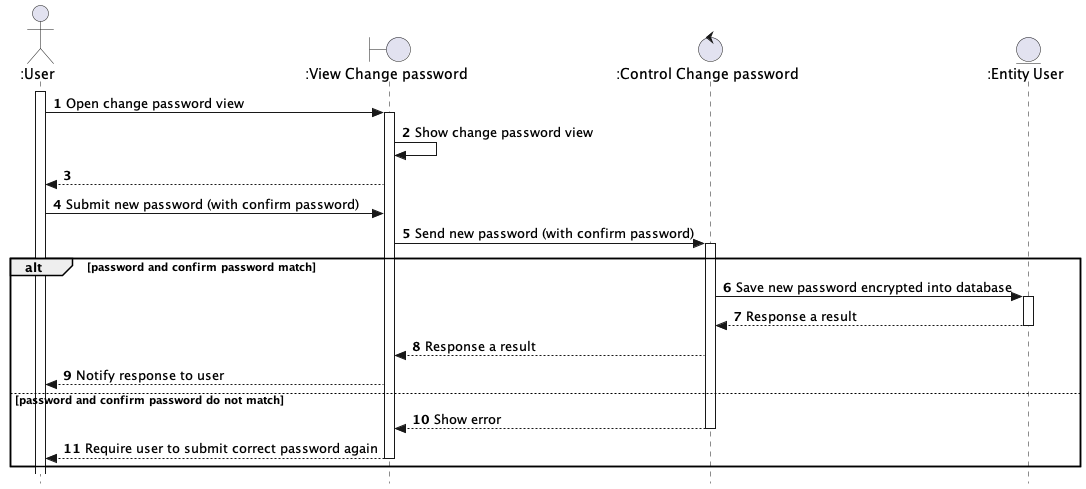
\includegraphics[width=16cm,height=9cm]{Images/mobile_app/change_password.png}
        \caption[Sơ đồ tuần tự chức năng đổi mật khẩu trên App]{\bfseries \fontsize{12pt}{0pt}
        \selectfont Sơ đồ tuần tự chức năng đổi mật khẩu trên App}
        \label{change_password} %đặt tên cho ảnh
  \end{figure}

  Sơ đồ tuần tự trên mô tả chi tiết quá trình người dùng đổi mật khẩu. Người dùng nhập mật khẩu và gửi yêu cầu đổi mật khẩu, 
  yêu cầu sẽ được xử lý bởi Control, nếu có lỗi phát sinh sẽ trả ra lỗi cho người dùng và yêu cầu người dùng nhập lại. Control
  sẽ xử lý cụ thể như thế nào được chúng em thể hiện trong Hình \ref{changePassword} trong chương sau.

\subsubsection{Sơ đồ tuần tự chức năng xem/gửi tin nhắn}

  \begin{figure}[H]
        \centering
        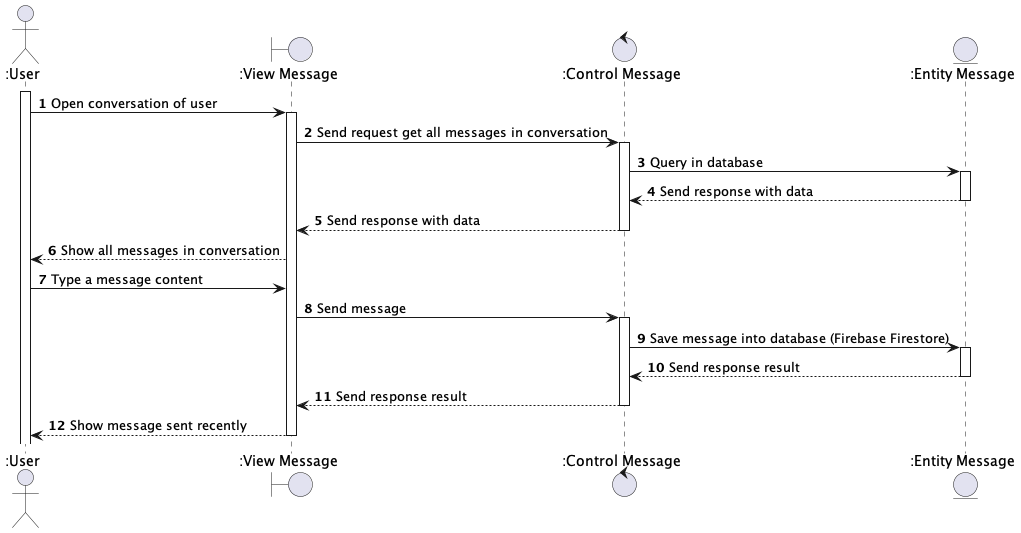
\includegraphics[width=16cm,height=11cm]{Images/mobile_app/send_and_receive_message.png}
        \caption[Sơ đồ tuần tự chức năng xem/gửi tin nhắn trên App]{\bfseries \fontsize{12pt}{0pt}
        \selectfont Sơ đồ tuần tự chức năng xem/gửi tin nhắn trên App}
        \label{send_and_receive_message} %đặt tên cho ảnh
  \end{figure}

  Sơ đồ tuần tự trên mô tả chi tiết quá trình người dùng xem và gửi tin nhắn. Người dùng click vào hội thoại để xem tin nhắn. 
  Nếu người dùng gửi tin nhắn, Control sẽ xử lý để gửi tin nhắn đến cho đối phương và lưu tin nhắn vào cơ sở dữ liệu. Ở chức năng
  này chúng em sử dụng Firebase để xử lý tất cả các tin nhắn, việc sử dụng Firebase sẽ được chúng em giới thiệu ở chương sau.

\subsubsection{Sơ đồ tuần tự chức năng xem bài đăng tin tức}

  \begin{figure}[H]
        \centering
        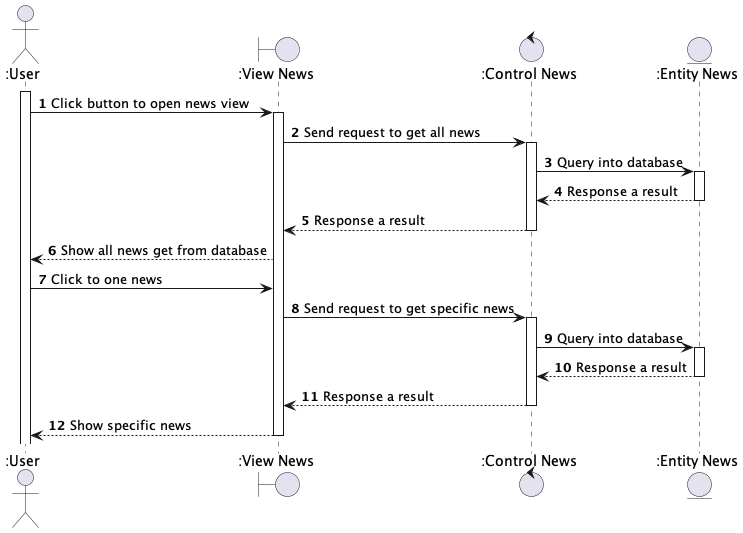
\includegraphics[width=15cm,height=8cm]{Images/mobile_app/view_news.png}
        \caption[ Sơ đồ tuần tự chức năng xem bài đăng tin tứctrên App]{\bfseries \fontsize{12pt}{0pt}
        \selectfont Sơ đồ tuần tự chức năng xem bài đăng tin tức trên App}
        \label{view_news} %đặt tên cho ảnh
  \end{figure}

  Sơ đồ tuần tự trên mô tả chi tiết quá trình người dùng xem tin tức/bài đăng. Người dùng chọn mở giao diện tin tức, API lấy tin tức sẽ
  được xử lý bởi Control, và hiện danh sách các bài đăng cho người dùng, sau đó người dùng chọn một bài đăng thì thông tin chi tiết
  của bài đăng sẽ hiển thị cho người dùng. Cụ thể về việc xử lý các yêu cầu của Control được chúng em thể hiện trong 
  Hình \ref{getAllNews}, Hình \ref{getNewsByCategory} trong chương sau.

\subsubsection{Sơ đồ tuần tự chức năng bật/tắt Bluetooth}

  \begin{figure}[H]
        \centering
        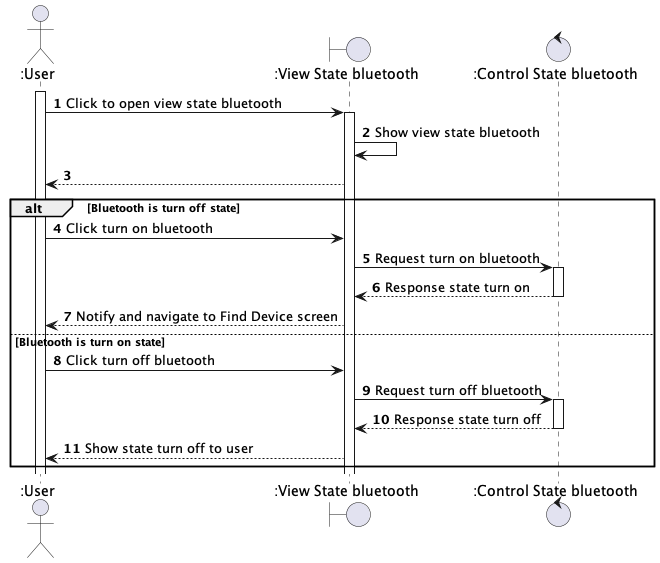
\includegraphics[width=14cm,height=10cm]{Images/mobile_app/turn_on_off_bluetooth.png}
        \caption[Sơ đồ tuần tự chức năng bật/tắt Bluetooth trên App]{\bfseries \fontsize{12pt}{0pt}
        \selectfont Sơ đồ tuần tự chức năng bật/tắt Bluetooth trên App}
        \label{turn_on_off_bluetooth} %đặt tên cho ảnh
  \end{figure}

  Sơ đồ tuần tự trên mô tả chi tiết quá trình bật/tắt Bluetooth. Người dùng gửi yêu cầu bật hoặc tắt Bluetooth, Control sẽ kiểm tra
  trạng thái Bluetooth và truy cập vào phần cứng thực hiện yêu cầu của người dùng.

\subsubsection{Sơ đồ tuần tự chức năng kết nối Bluetooth với thiết bị đo điện tim}

  \begin{figure}[H]
        \centering
        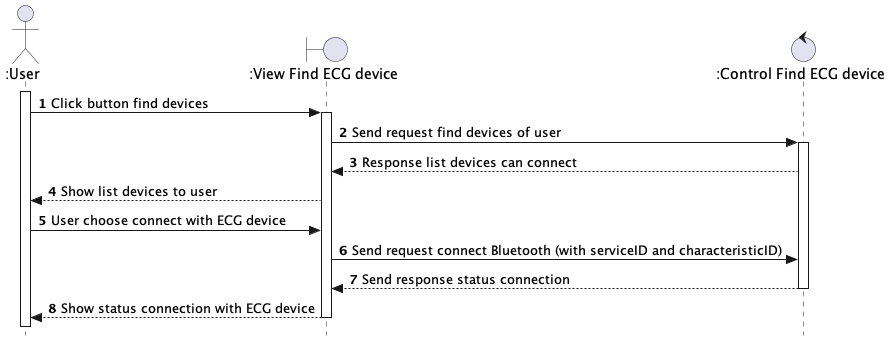
\includegraphics[width=14cm,height=6cm]{Images/mobile_app/connect_with_device.png}
        \caption[Sơ đồ tuần tự chức năng kết nối Bluetooth với thiết bị đo điện tim trên App]{\bfseries \fontsize{12pt}{0pt}
        \selectfont Sơ đồ tuần tự chức năng kết nối Bluetooth với thiết bị đo điện tim trên App}
        \label{connect_with_device} %đặt tên cho ảnh
  \end{figure}

  Sơ đồ tuần tự trên mô tả chi tiết quá trình người dùng kết nối với thiết bị đo điện tim. Người dùng sau khi bật Bluetooth
  sẽ có thể tìm kiếm thiết bị và xem các danh sách các thiết bị mình tìm thấy. Người dùng chọn đúng thiết bị (theo tên) 
  và thực hiện kết nối, kết quả của việc kết nối sẽ được hiện trên màn hình.

\subsubsection{Sơ đồ tuần tự chức năng ngắt kết nối Bluetooth với thiết bị đo điện tim}

  \begin{figure}[H]
        \centering
        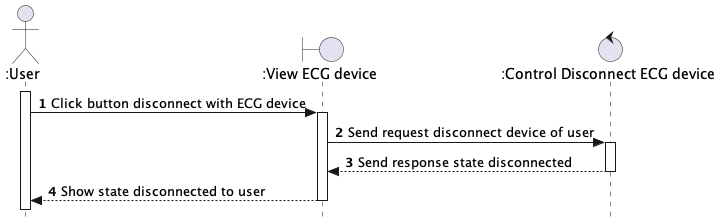
\includegraphics[width=12cm,height=3.5cm]{Images/mobile_app/disconnect_with_device.png}
        \caption[Sơ đồ tuần tự chức năng ngắt kết nối Bluetooth với thiết bị đo điện tim trên App]{\bfseries \fontsize{12pt}{0pt}
        \selectfont Sơ đồ tuần tự chức năng ngắt kết nối Bluetooth với thiết bị đo điện tim trên App}
        \label{disconnect_with_device} %đặt tên cho ảnh
  \end{figure}

  Sơ đồ tuần tự trên mô tả chi tiết quá trình người dùng ngắt kết nối với thiết bị đo điện tim. Trong khi đang kết nối, người dùng
  có thể chọn ngắt kết nối Bluetooth giữa thiết bị và ứng dụng, sau khi ngắt kết nối, sẽ có thông báo
  hiển thị trên màn hình.

\subsubsection{Sơ đồ tuần tự chức năng tiến hành đo điện tim}

  \begin{figure}[H]
        \centering
        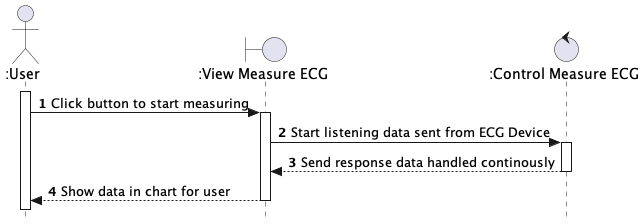
\includegraphics[width=12cm,height=6cm]{Images/mobile_app/start_measuring_ecg.png}
        \caption[Sơ đồ tuần tự chức năng tiến hành đo điện tim trên App]{\bfseries \fontsize{12pt}{0pt}
        \selectfont Sơ đồ tuần tự chức năng tiến hành đo điện tim trên App}
        \label{start_measuring_ecg} %đặt tên cho ảnh
  \end{figure}
 
  Sơ đồ tuần tự trên mô tả chi tiết quá trình người dùng bắt đầu quá trình đo điện tim. Để bắt đầu được quá trình đo, điều
  kiện đó là người dùng đã kết nối thiết bị với ứng dụng để có thể lắng nghe được dữ liệu từ Bluetooth trả ra. Sau khi nhấn nút bắt đầu đo,
  dữ liệu lắng nghe sẽ được xử lý và thể hiện trên biểu đồ cho người dùng.

\subsubsection{Sơ đồ tuần tự chức năng kết thúc quá trình đo điện tim}

  \begin{figure}[H]
        \centering
        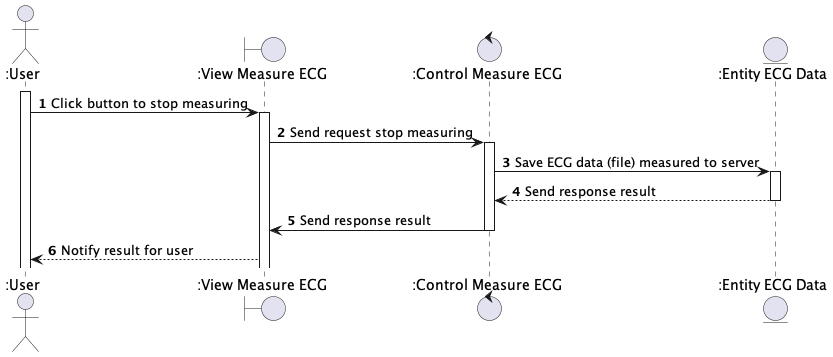
\includegraphics[width=12cm,height=5cm]{Images/mobile_app/end_measuring_ecg.png}
        \caption[Sơ đồ tuần tự chức năng kết thúc quá trình đo điện tim trên App]{\bfseries \fontsize{12pt}{0pt}
        \selectfont Sơ đồ tuần tự chức năng kết thúc quá trình đo điện tim trên App}
        \label{end_measuring_ecg} %đặt tên cho ảnh
  \end{figure}

  Sơ đồ tuần tự trên mô tả chi tiết quá trình người dùng kết thúc quá trình đo điện tim. Trong khi đang đo, nếu người dùng muốn dừng, 
  việc kết thúc quá trình đo đồng nghĩa với dữ liệu đo được lưu lên cơ sở dữ liệu để bác sĩ có thể theo dõi.

\subsection{Phân tích dữ liệu}

Tại phần này, chúng em sẽ tiến hành xác định và mô tả các thực thể cũng như
 thuộc tính quan trọng trong hệ thống. Việc này giúp chúng ta có cái
  nhìn tổng quan về các yếu tố chính cần được quản lý và lưu trữ
   trong cơ sở dữ liệu. Bằng cách làm điều này, chúng ta có thể
    xây dựng một mô hình dữ liệu cơ bản để hỗ trợ việc thiết kế và
     triển khai hệ thống một cách hiệu quả.

     Trước hết, chúng em sẽ xác định và mô tả các thực thể chính trong hệ
      thống. Thực thể là các đối tượng hoặc khái niệm quan
       trọng mà chúng ta cần theo dõi và quản lý. Sau đó, chúng ta sẽ xác
        định các thuộc tính liên quan đến mỗi thực thể, các thông tin cần
         được lưu trữ và quản lý.

\begin{table}[H]
  \caption{\bfseries \fontsize{12pt}{0pt}\selectfont Bảng thực thể và thuộc tính}
  \centering
  \begin{tabularx}{0.9\textwidth}{|c|X|}
    \hline
    \textbf{Thực thể} & \textbf{Thuộc tính} \\
    \hline
    Người dùng & 
    ID người dùng, Mật khẩu, Email, Tên, Ngày sinh, Số điện thoại, Quyền \\
    \hline
    Bản ghi ECG & 
    ID bản ghi ECG, ID người dùng, ID thiết bị, Đường dẫn lưu trữ dữ liệu, Thời gian bắt đầu đo, Thời gian kết thúc đo, Loại cảm biến \\
    \hline
    Danh mục tin tức & 
    ID danh mục tin tức, Tên danh mục tin tức, Mô tả danh mục tin tức \\
    \hline
    Tin tức & 
    ID tin tức, Tiêu đề, Nội dung, ID danh mục tin tức, Tác giả, Đường dẫn, Đường dẫn hình ảnh \\
    \hline
    Phân công bệnh nhân - bác sĩ & 
    ID phân công, ID bệnh nhân, ID bác sĩ, Ngày bắt đầu \\
    \hline
    Mã thông báo đặt lại mật khẩu & 
    ID mã thông báo, ID người dùng, Mã thông báo, Thời gian hết hạn \\
    \hline
    Phiên đăng nhập & 
    ID phiên đăng nhập, ID người dùng, Mã phiên đăng nhập, Thời gian hết hạn \\
    \hline
    Thiết bị & 
    ID thiết bị, Tên thiết bị \\
    \hline
    Thông tin hội thoại & 
    ID hội thoại, Danh sách ID người dùng trong hội thoại, thông tin tin nhắn gần nhất \\
    \hline
    Tin nhắn & 
    ID tin nhắn, Nội dung tin nhắn, ID người gửi tin nhắn, thời gian gửi tin nhắn \\
    \hline
    Firebase token người dùng & 
    ID token, Firebase token, ID người dùng \\
    \hline
  \end{tabularx}

  
\end{table}
Sau khi hoàn thành được bảng thực thể và thuộc tính, chúng em xác định được mô hình thực thể liên kết như sau:

\begin{figure}[H]
  \centering
  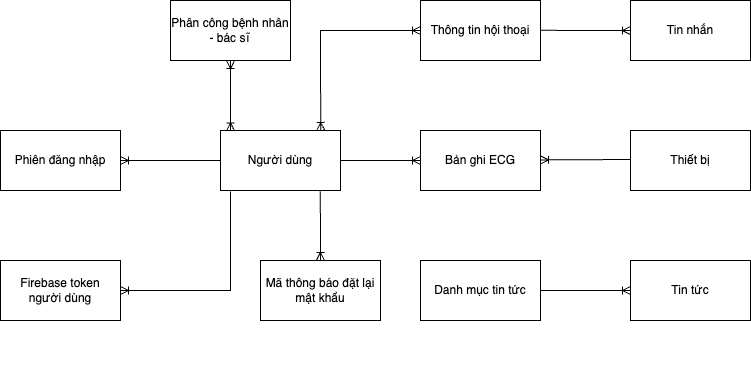
\includegraphics[width=15cm,height=8cm]{Images/system/fmECG_connection_entity.png}
  \caption[Mô hình thực thể liên kết]{\bfseries \fontsize{12pt}{0pt}
  \selectfont Mô hình thực thể liên kết}
  \label{ttlk} %đặt tên cho ảnh
\end{figure}


\subsection{Kết luận chương}

Trong chương này, chúng em đã thực hiện phân tích toàn diện về
 hệ thống cho đề tài , nhằm đáp ứng
  các mục tiêu và yêu cầu đã được đề xuất.

Chúng em đã xác định rõ ràng các khía cạnh quan trọng của hệ thống,
 tập trung vào việc thiết kế một hệ thống quản lý ECG hiệu quả,
  trực quan và có khả năng theo dõi sức khỏe tim mạch một cách
   chính xác. 


\newpage


\section*{CHƯƠNG 2. THIẾT KẾ CHI TIẾT HỆ THỐNG}
\setcounter{section}{2}
\setcounter{subsection}{0} %LƯU Ý MỖI LẦN THÊM CHƯƠNG MỚI CẦN THÊM CÂU NÀY ĐỂ RESET THỨ TỰ CỦA SUBSECTON VỀ 1
\setcounter{table}{0} % LƯU Ý SAU MỖI LẦN GỌI BẢNG HAY HÌNH ẢNH PHẢI THÊM CÂU NÀY ĐỂ RESET THỨ TỰ
\setcounter{figure}{0} %% LƯU Ý SAU MỖI LẦN GỌI BẢNG HAY HÌNH ẢNH PHẢI THÊM CÂU NÀY ĐỂ RESET THỨ TỰ
\addcontentsline{toc}{section}{\numberline{}CHƯƠNG 2. THIẾT KẾ CHI TIẾT HỆ THỐNG}

\subsection{Sơ đồ kiến trúc hệ thống}
Hệ thống chúng em xây dựng được chia làm ba phần Device, Application và Server. Các chi tiết cụ thể được thể hiện trong
hình vẽ:

\begin{figure}[H]
  \centering
  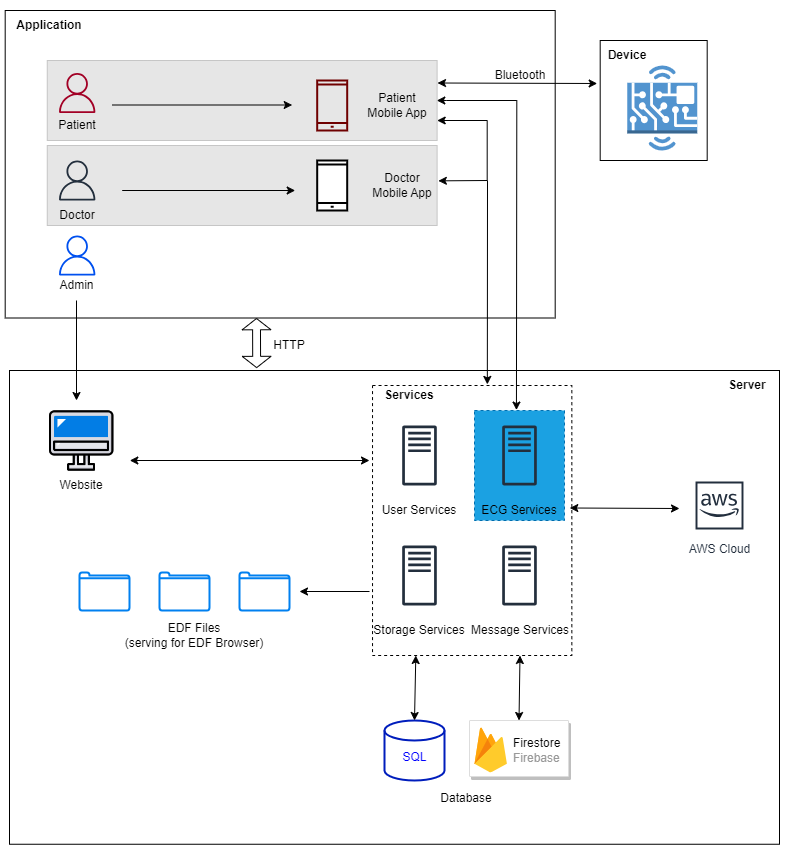
\includegraphics[width=16cm,height=18cm]{Images/system/fmECG_architecture-System Architecture.drawio.png}
  \caption[Kiến trúc tổng quan hệ thống]{\bfseries \fontsize{12pt}{0pt}\selectfont Kiến trúc tổng quan hệ thống}
  \label{fmECG_architecture-System} %đặt tên cho ảnh
\end{figure}

Hình \ref{fmECG_architecture-System} thể hiện ba phần: 
\begin{itemize}
  \item Device: Thiết bị phần cứng đo điện tim, để kết nối với App bệnh nhân thông qua Bluetooth 
  \item Application: Bao gồm ứng dụng của bệnh nhân, ứng dụng của bác sĩ và Website của Admin
  \item Server: Bao gồm các Services để xử lý các yêu cầu gửi từ Application, cơ sở dữ liệu và Cloud lưu trữ
\end{itemize}

Trong hệ thống thì Devices là phần mà chúng em sẽ không trực tiếp thực hiện trong đồ án này, Application và Server sẽ là
phần mà đồ án chúng em thực hiện. Ở trong sơ đồ kiến trúc hệ thống riêng có bệnh nhân sẽ có tương tác trực tiếp với Devices,
còn lại khối Application sẽ tương tác với Server thông qua API với giao thức HTTP. Khi nhận được yêu cầu từ Application,
Server sẽ thực hiện xử lý dữ liệu, mọi yêu cầu đến đều được xử lý bởi Services, tuỳ vào yêu cầu đến Services tương ứng sẽ đảm nhiệm 
việc lấy/lưu dữ liệu trong cơ sở dữ liệu sau đó trả ra kết quả cho người dùng.

Ngoài ra, hệ thống sẽ phải có kết nối bluetooth low energy giữa thiết bị đo và ứng dụng di động để có thể truyền/nhận dữ liệu.
Trên đây là tổng quan về kiến trúc hệ thống, phần tiếp dưới đây chúng em xin phép trình bày kỹ hơn về từng khối nhỏ hơn
dựa vào những đối tượng đã được xác định trong hệ thống.

\subsection{Sơ đồ khối phần mềm}

\subsubsection{Ứng dụng di động cho bệnh nhân}
\mbox{}

\begin{figure}[H]
  \centering
  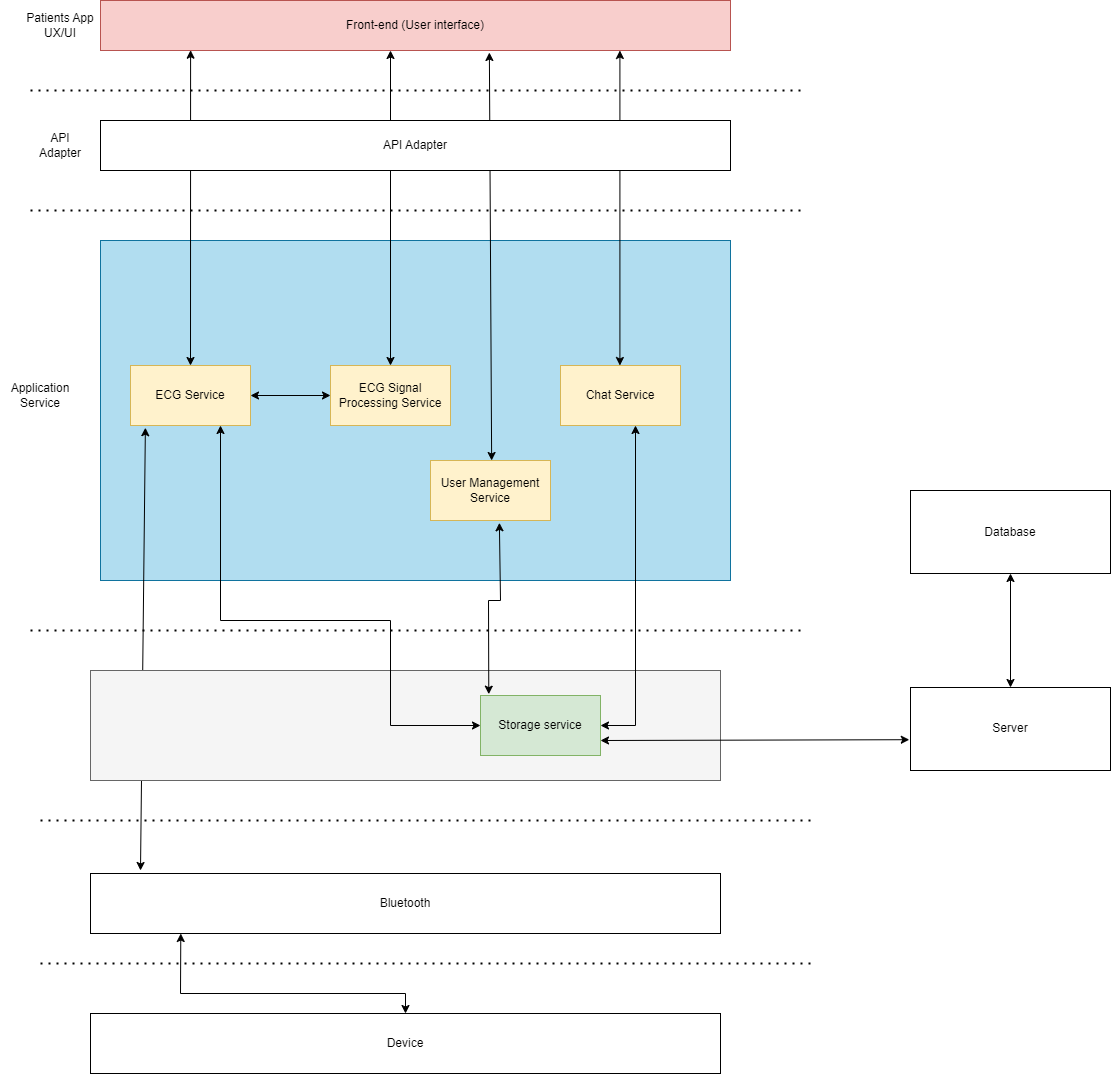
\includegraphics[width=16cm,height=18cm]{Images/system/fmECG_architecture-Patient.drawio.png}
  \caption[Sơ đồ khối cho App bệnh nhân]{\bfseries \fontsize{12pt}{0pt}\selectfont Sơ đồ khối cho App bệnh nhân}
  \label{fmECG_architecture-Patient} %đặt tên cho ảnh
\end{figure}

Trong hình trên, lớp trên cùng User interface là lớp để người dùng tương tác và thực hiện lời gọi thông qua API Adapter, 
các yêu cầu của người dùng sẽ được xử lý thông qua Services và phản hồi lại với người dùng qua giao diện. Dưới đây là phần
giải thích Services trong hình:

\begin{itemize}
  \item ECG Service: Khối có nhiệm vụ xử lý yêu cầu cho các trạng thái đo: thực hiện đo, kết thúc đo, lưu kết quả đo
  \item ECG Signal Processing Service: Khối có nhiệm vụ xử lý tín hiệu đo để phân tích sâu, hiển thị lên màn hình
  \item User Management Service: Khối có nhiệm vụ xử lý các vấn đề liên quan đến người dùng như đăng nhập, đăng ký
  \item Chat Service: Khối có nhiệm vụ quản lý việc chat, trao đổi thông tin
  \item Storage Service: Khối có nhiệm vụ lưu thông tin vào bộ nhớ
\end{itemize}

Riêng với App cho bệnh nhân thì sẽ có Khối Bluetooth và Khối Device để phục vụ cho việc đo điện tim.
\subsubsection{Ứng dụng di động cho bác sĩ}

\begin{figure}[H]
  \centering
  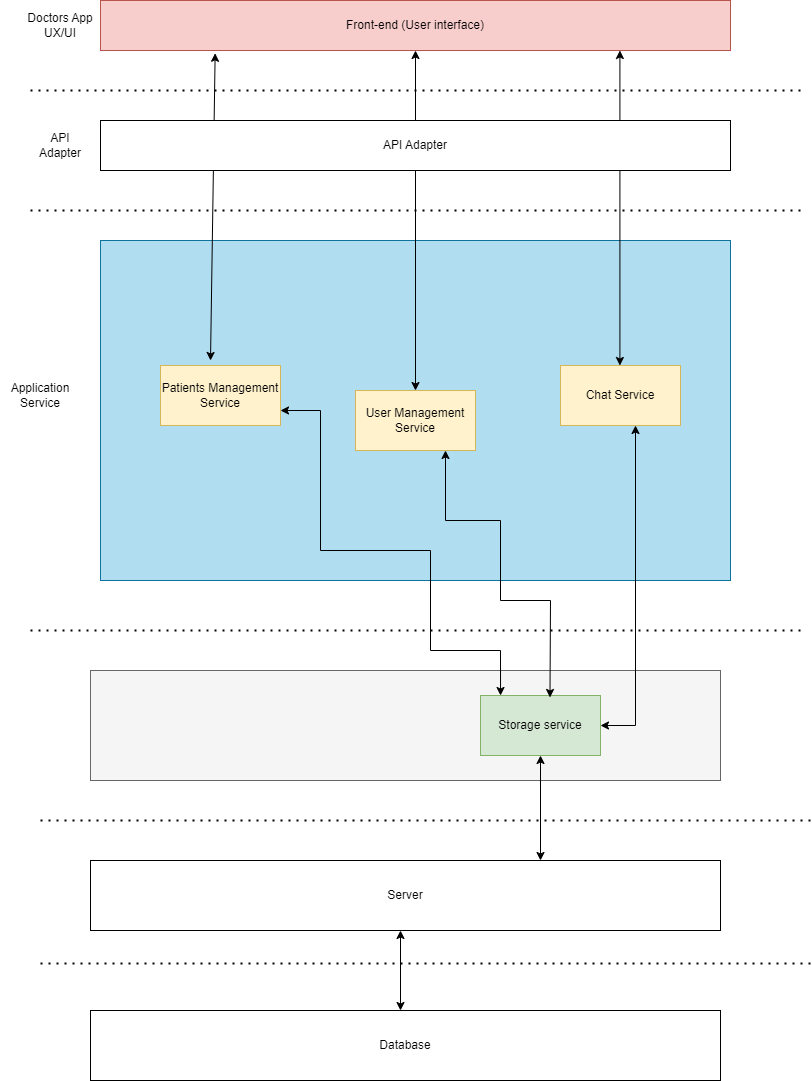
\includegraphics[width=16cm,height=18cm]{Images/system/fmECG_architecture-Doctors.drawio.png}
  \caption[Sơ đồ khói cho App bác sĩ]{\bfseries \fontsize{12pt}{0pt}\selectfont Sơ đồ khối cho App bác sĩ}
  \label{fmECG_architecture-Doctors} %đặt tên cho ảnh
\end{figure}

Về cơ bản, ứng dụng di động cho bác sĩ có những khối tương tự với bệnh nhân, trừ việc bác sĩ sẽ không có hai khối Device
và Bluetooth để phục vụ việc đo như bệnh nhân.


\subsubsection{Website cho quản trị viên}

\begin{figure}[H]
  \centering
  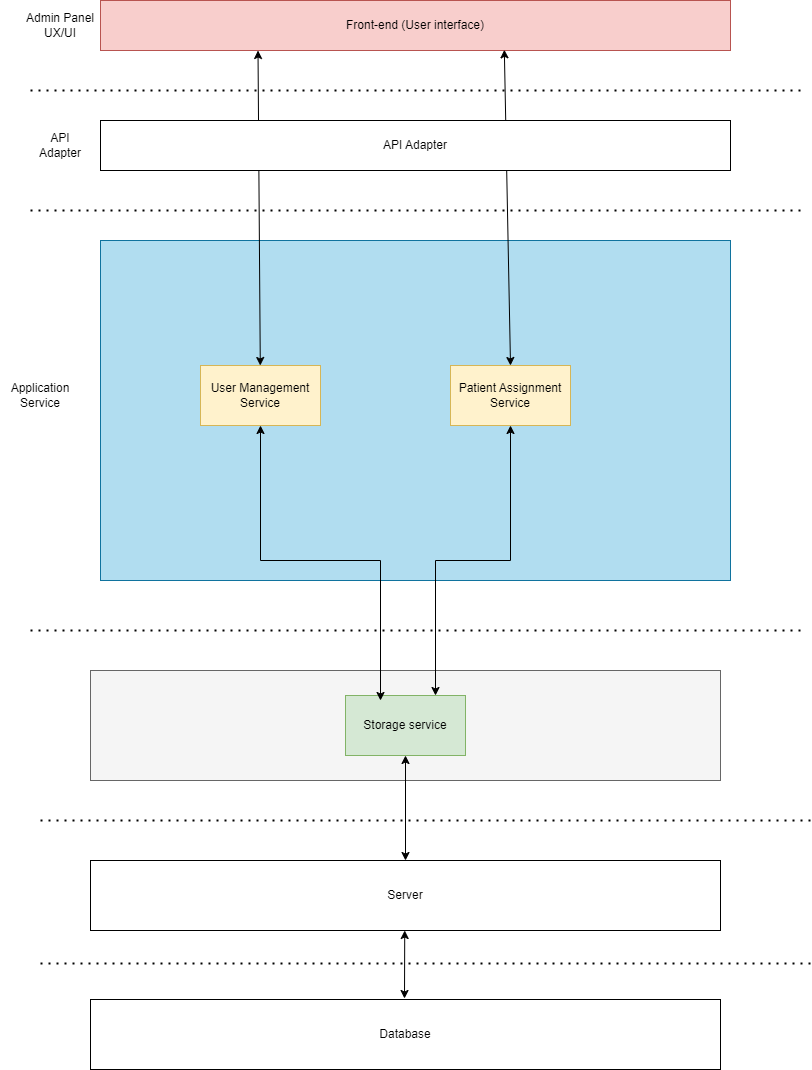
\includegraphics[width=16cm,height=18cm]{Images/system/fmECG_architecture-Admin.drawio.png}
  \caption[Sơ đồ khối cho Website quản trị viên]{\bfseries \fontsize{12pt}{0pt}\selectfont Sơ đồ khối cho Website quản trị viên}
  \label{fmECG_architecture-Admin} %đặt tên cho ảnh
\end{figure}

Quản trị viên sẽ quản lý 2 Services chính đó là quản lý người dùng (User Management Service) và quản lý phân công
bác sĩ - bệnh nhân (Patient Assignment Service), logic và thứ tự các khối tương đồng với ứng dụng dành cho bác sĩ.

Tiếp theo để phân tích cụ thể hơn từng luồng trong hệ thống qua use case, chúng em xin phép được trình bày các sơ đồ tuần
tự. 
\newpage


\subsection{Thiết kế cơ sở dữ liệu}
\label{design_database}


\subsubsection{Chuyển mô hình thực thể liên kết sang mô hình quan hệ}

\begin{itemize}
  \item Người dùng (\textbf{ID người dùng}, Mật khẩu, Email, Tên, Ngày sinh, Số điện thoại, Quyền)
  \item Bản ghi ECG (\textbf{ID bản ghi ECG}, ID người dùng, ID thiết bị, Đường dẫn lưu trữ dữ liệu, Thời gian bắt đầu đo, Thời gian kết thúc đo, Loại cảm biến)
  \item Danh mục tin tức (\textbf{ID danh mục tin tức}, Tên danh mục tin tức, Mô tả danh mục tin tức)
  \item Tin tức (\textbf{ID tin tức}, Tiêu đề, Nội dung, ID danh mục tin tức, Tác giả, Đường dẫn, Đường dẫn hình ảnh)
  \item Phân công bệnh nhân - bác sĩ (\textbf{ID phân công}, ID bệnh nhân, ID bác sĩ, Ngày bắt đầu)
  \item Mã thông báo đặt lại mật khẩu (\textbf{ID mã thông báo}, ID người dùng, Mã thông báo, Thời gian hết hạn)
  \item Phiên đăng nhập (\textbf{ID phiên đăng nhập}, ID người dùng, Mã phiên đăng nhập, Thời gian hết hạn)
  \item Thiết bị (\textbf{ID thiết bị}, Tên thiết bị)
\end{itemize}



\subsubsection{Mối quan hệ dữ liệu}

\begin{itemize}
  \item Bảng \texttt{ecg\_record} có mối quan hệ 1-n với bảng \texttt{user} thông qua khóa ngoại \texttt{user\_id}.
  \item Bảng \texttt{news} có mối quan hệ n-1 với bảng \texttt{news\_category} thông qua khóa ngoại \texttt{category\_id}.
  \item Bảng \texttt{patient\_doctor\_assignment} có mối quan hệ n-1 với bảng \texttt{user} thông qua khóa ngoại \texttt{patient\_id} và \texttt{doctor\_id}.
  \item Bảng \texttt{reset\_token} có mối quan hệ n-1 với bảng \texttt{user} thông qua khóa ngoại \texttt{user\_id}.
\end{itemize}

\subsubsection{Chuẩn hoá 3NF}
Các bảng đã được thiết kế theo nguyên tắc chuẩn hoá 3NF, vì không có thuộc tính lặp lại và các thuộc tính không phụ thuộc vào một tập hợp con của khóa chính.

\paragraph{Chuẩn hoá bảng Người dùng}
\mbox{}

\begin{table}[H]
  \caption{\bfseries \fontsize{12pt}{0pt}\selectfont Bảng chuẩn hoá bảng Người dùng}
  \centering
  \begin{tabularx}{0.9\textwidth}{|X|X|}
    \hline
    \textbf{Danh sách thuộc tính} & ID người dùng, Mật khẩu, Email, Tên, Ngày sinh, Số điện thoại,
    Quyền \\ % Thêm \textbf{} cho abc
    \hline
    \textbf{Quy tắc nghiệp vụ} & \textbf{Phụ thuộc hàm} \\
    \hline
    Mỗi người dùng có một ID riêng, có duy nhất mật khẩu, email, tên, ngày sinh, số điện thoại,
    quyền & \parbox[t]{\linewidth}{$\text{ID người dùng} \rightarrow$ mật khẩu, email, tên, ngày sinh, số điện thoại, quyền} \\
    \hline
    \multicolumn{2}{|X|}{$\Rightarrow \text{Khoá chính của bảng: ID người dùng}$} \\
    \multicolumn{2}{|X|}{$\Rightarrow \text{Bảng Người dùng đã ở 3NF}$} \\
    \hline
  \end{tabularx}
\end{table}


\paragraph{Chuẩn hoá bảng Bản ghi ECG}
\mbox{}

\begin{table}[H]
  \caption{\bfseries \fontsize{12pt}{0pt}\selectfont Bảng chuẩn hoá bảng Bản ghi ECG}
  \centering
  \begin{tabularx}{0.9\textwidth}{|X|X|}
    \hline
    \textbf{Danh sách thuộc tính} & ID bản ghi ECG, ID người dùng, ID thiết bị, Đường dẫn lưu trữ dữ
    liệu, Thời gian bắt đầu đo, Thời gian kết thúc đo, Loại cảm biến \\
    \hline
    \textbf{Quy tắc nghiệp vụ} & \textbf{Phụ thuộc hàm} \\
    \hline
    Mỗi bản ghi ECG có một ID riêng, có duy nhất ID người dùng, ID thiết bị, đường dẫn lưu trữ dữ
    liệu, thời gian bắt đầu đo, thời gian kết thúc đo, loại cảm biến & \parbox[t]{\linewidth}{$ \text{ID bản ghi ECG} \rightarrow$ ID người dùng, ID thiết bị, đường dẫn lưu trữ dữ
    liệu, thời gian bắt đầu đo, thời gian kết thúc đo, loại cảm biến} \\
    \hline
    \multicolumn{2}{|X|}{$\Rightarrow \text{Khoá chính của bảng: ID bản ghi ECG}$} \\
    \multicolumn{2}{|X|}{$\Rightarrow \text{Bảng Bản ghi ECG đã ở 3NF}$} \\
    \hline
  \end{tabularx}
\end{table}


\paragraph{Chuẩn hoá bảng Danh mục tin tức}
\mbox{}


\begin{table}[H]
  \caption{\bfseries \fontsize{12pt}{0pt}\selectfont Bảng chuẩn hoá bảng Danh mục tin tức}
  \centering
  \begin{tabularx}{0.9\textwidth}{|X|X|}
    \hline
    \textbf{Danh sách thuộc tính} & ID danh mục tin tức, Tên danh mục tin tức, Mô tả danh mục tin
    tức \\ % Thêm \textbf{} cho abc
    \hline
    \textbf{Quy tắc nghiệp vụ} & \textbf{Phụ thuộc hàm} \\
    \hline
    Mỗi danh mục tin tức có một ID riêng, có duy nhất tên danh mục tin tức, mô tả danh mục tin
    tức & \parbox[t]{\linewidth}{$\text{ID danh mục tin tức} \rightarrow$ danh mục tin tức, mô tả danh mục tin
    tức} \\
    \hline
    \multicolumn{2}{|X|}{$\Rightarrow \text{Khoá chính của bảng: ID danh mục tin tức}$} \\
    \multicolumn{2}{|X|}{$\Rightarrow \text{Bảng Danh mục tin tức đã ở 3NF}$} \\
    \hline
  \end{tabularx}
\end{table}


\paragraph{Chuẩn hoá bảng Tin tức}
\mbox{}

\begin{table}[H]
  \caption{\bfseries \fontsize{12pt}{0pt}\selectfont Bảng chuẩn hoá bảng Tin tức}
  \centering
  \begin{tabularx}{0.9\textwidth}{|X|X|}
    \hline
    \textbf{Danh sách thuộc tính} & ID tin tức, Tiêu đề, Nội dung, ID danh mục tin tức, Tác giả, Đường dẫn,
    Đường dẫn hình ảnh \\ % Thêm \textbf{} cho abc
    \hline
    \textbf{Quy tắc nghiệp vụ} & \textbf{Phụ thuộc hàm} \\
    \hline
    Mỗi tin tức có một ID riêng, có duy nhất tiêu đề, nội dung, ID danh mục tin tức, tác giả, đường dẫn,
    đường dẫn hình ảnh & \parbox[t]{\linewidth}{$\text{ID tin tức} \rightarrow$ tiêu đề, nội dung, ID danh mục tin tức, tác giả, đường dẫn,
    đường dẫn hình ảnh} \\
    \hline
    \multicolumn{2}{|X|}{$\Rightarrow \text{Khoá chính của bảng: ID tin tức}$} \\
    \multicolumn{2}{|X|}{$\Rightarrow \text{Bảng Tin tức đã ở 3NF}$} \\
    \hline
  \end{tabularx}
\end{table}



\paragraph{Chuẩn hoá bảng Phân công bệnh nhân - bác sĩ}
\mbox{}

\begin{table}[H]
  \caption{\bfseries \fontsize{12pt}{0pt}\selectfont Bảng chuẩn hoá bảng Phân công bệnh nhân - bác sĩ}
  \centering
  \begin{tabularx}{0.9\textwidth}{|X|X|}
    \hline
    \textbf{Danh sách thuộc tính} & ID phân công, ID bệnh nhân, ID bác sĩ, Ngày bắt
    đầu \\ % Thêm \textbf{} cho abc
    \hline
    \textbf{Quy tắc nghiệp vụ} & \textbf{Phụ thuộc hàm} \\
    \hline
    Mỗi lần phân công bệnh nhân - bác sĩ có một ID riêng, có duy nhất ID bệnh nhân, ID bác sĩ, ngày bắt
    đầu & \parbox[t]{\linewidth}{$\text{ID phân công} \rightarrow$ ID bệnh nhân, ID bác sĩ, ngày bắt
    đầu} \\
    \hline
    \multicolumn{2}{|X|}{$\Rightarrow \text{Khoá chính của bảng: ID phân công}$} \\
    \multicolumn{2}{|X|}{$\Rightarrow \text{Bảng Phân công bệnh nhân - bác sĩ đã ở 3NF}$} \\
    \hline
  \end{tabularx}
\end{table}




\paragraph{Chuẩn hoá bảng Mã thông báo đặt lại mật khẩu}
\mbox{}

\begin{table}[H]
  \caption{\bfseries \fontsize{12pt}{0pt}\selectfont Bảng chuẩn hoá bảng Mã thông báo đặt lại mật khẩu}
  \centering
  \begin{tabularx}{0.9\textwidth}{|X|X|}
    \hline
    \textbf{Danh sách thuộc tính} & ID mã thông báo, ID người dùng, Mã thông báo,
    Thời gian hết hạn \\ % Thêm \textbf{} cho abc
    \hline
    \textbf{Quy tắc nghiệp vụ} & \textbf{Phụ thuộc hàm} \\
    \hline
    Mỗi mã thông báo đặt lại mật khẩu có một ID riêng, có duy nhất ID người dùng, mã thông báo,
    thời gian hết hạn & \parbox[t]{\linewidth}{$\text{ID mã thông báo} \rightarrow$ ID người dùng, mã thông báo,
    thời gian hết hạn} \\
    \hline
    \multicolumn{2}{|X|}{$\Rightarrow \text{Khoá chính của bảng: ID mã thông báo}$} \\
    \multicolumn{2}{|X|}{$\Rightarrow \text{Bảng Mã thông báo đặt lại mật khẩu đã ở 3NF}$} \\
    \hline
  \end{tabularx}
\end{table}


\paragraph{Chuẩn hoá bảng Phiên đăng nhập}
\mbox{}

\begin{table}[H]
  \caption{\bfseries \fontsize{12pt}{0pt}\selectfont Bảng chuẩn hoá bảng Phiên đăng nhập}
  \centering
  \begin{tabularx}{0.9\textwidth}{|X|X|}
    \hline
    \textbf{Danh sách thuộc tính} & ID phiên đăng nhập, ID người dùng, Mã phiên đăng nhập, Thời
    gian hết hạn \\ % Thêm \textbf{} cho abc
    \hline
    \textbf{Quy tắc nghiệp vụ} & \textbf{Phụ thuộc hàm} \\
    \hline
    Mỗi phiên đăng nhập có một ID riêng, có duy nhất ID người dùng, mã phiên đăng nhập, thời
    gian hết hạn & \parbox[t]{\linewidth}{$\text{ID phiên đăng nhập} \rightarrow$ ID người dùng, mã phiên đăng nhập, thời
    gian hết hạn} \\
    \hline
    \multicolumn{2}{|X|}{$\Rightarrow \text{Khoá chính của bảng: ID phiên đăng nhập}$} \\
    \multicolumn{2}{|X|}{$\Rightarrow \text{Bảng Phiên đăng nhập đã ở 3NF}$} \\
    \hline
  \end{tabularx}
\end{table}



\paragraph{Chuẩn hoá bảng Thiết bị}
\mbox{}

\begin{table}[H]
  \caption{\bfseries \fontsize{12pt}{0pt}\selectfont Bảng chuẩn hoá bảng Thiết bị}
  \centering
  \begin{tabularx}{0.9\textwidth}{|X|X|}
    \hline
    \textbf{Danh sách thuộc tính} & ID thiết bị, Tên thiết bị \\ % Thêm \textbf{} cho abc
    \hline
    \textbf{Quy tắc nghiệp vụ} & \textbf{Phụ thuộc hàm} \\
    \hline
    Mỗi thiết bị có một ID riêng, có duy nhất tên thiết bị & \parbox[t]{\linewidth}{$\text{ID thiết bị} \rightarrow$ tên thiết bị} \\
    \hline
    \multicolumn{2}{|X|}{$\Rightarrow \text{Khoá chính của bảng: ID thiết bị}$} \\
    \multicolumn{2}{|X|}{$\Rightarrow \text{Bảng Thiết bị đã ở 3NF}$} \\
    \hline
  \end{tabularx}
\end{table}




\subsubsection{Từ điển dữ liệu}



\begin{table}[H]
  \caption{\bfseries \fontsize{12pt}{0pt}\selectfont Bảng user}
  \centering
  \begin{tabularx}{0.9\textwidth}{|c|c|X|}
    \hline
    \textbf{Thuộc tính} & \textbf{Kiểu dữ liệu} & \textbf{Mô tả} \\
    \hline
    user\_id & INTEGER & Khóa chính của bảng, đại diện cho ID người dùng. \\
    \hline
    password & STRING & Mật khẩu của người dùng. \\
    \hline
    email & STRING & Địa chỉ email của người dùng. \\
    \hline
    name & STRING & Tên của người dùng. \\
    \hline
    doB & DATE & Ngày sinh của người dùng. \\
    \hline
    phone\_number & STRING & Số điện thoại của người dùng. \\
    \hline
    role & INTEGER & Quyền của người dùng (0-patient, 1-doctor, 2-admin). \\
    \hline
    created\_at & DATE & Thời điểm thêm mới dữ liệu vào database. \\
    \hline
    updated\_at & DATE & Thời điểm cập nhật dữ liệu vào database. \\
    \hline
    
  \end{tabularx}
\end{table}

\begin{table}[H]
  \caption{\bfseries \fontsize{12pt}{0pt}\selectfont Bảng ecg\_record}
  \centering
  \begin{tabularx}{0.9\textwidth}{|c|c|X|}
    \hline
    \textbf{Thuộc tính} & \textbf{Kiểu dữ liệu} & \textbf{Mô tả} \\
    \hline
    record\_id & INTEGER & Khóa chính của bảng, đại diện cho ID bản ghi ECG. \\
    \hline
    user\_id & INTEGER & Khóa ngoại tham chiếu đến \texttt{user\_id} trong bảng \texttt{user}. \\
    \hline
    device\_id & STRING & ID thiết bị. \\
    \hline
    data\_directory & STRING & Đường dẫn lưu trữ dữ liệu. \\
    \hline
    start\_time & DATE & Thời gian bắt đầu ghi lại ECG. \\
    \hline
    stop\_time & DATE & Thời gian kết thúc ghi lại ECG. \\
    \hline
    sensor\_type & STRING & Loại cảm biến. \\
    \hline
    created\_at & DATE & Thời điểm thêm mới dữ liệu vào database. \\
    \hline
    updated\_at & DATE & Thời điểm cập nhật dữ liệu vào database. \\
    \hline
  \end{tabularx}
\end{table}

\begin{table}[H]
  \caption{\bfseries \fontsize{12pt}{0pt}\selectfont Bảng news\_category}
  \centering
  \begin{tabularx}{0.9\textwidth}{|c|c|X|}
    \hline
    \textbf{Thuộc tính} & \textbf{Kiểu dữ liệu} & \textbf{Mô tả} \\
    \hline
    category\_id & INTEGER & Khóa chính của bảng, đại diện cho ID danh mục tin tức. \\
    \hline
    category\_name & STRING & Tên danh mục tin tức. \\
    \hline
    category\_description & STRING & Mô tả danh mục tin tức. \\
    \hline
    created\_at & DATE & Thời điểm thêm mới dữ liệu vào database. \\
    \hline
    updated\_at & DATE & Thời điểm cập nhật dữ liệu vào database. \\
    \hline
  \end{tabularx}
\end{table}

\begin{table}[H]
  \caption{\bfseries \fontsize{12pt}{0pt}\selectfont Bảng news}
  \centering
  \begin{tabularx}{0.9\textwidth}{|c|c|X|}
    \hline
    \textbf{Thuộc tính} & \textbf{Kiểu dữ liệu} & \textbf{Mô tả} \\
    \hline
    news\_id & INTEGER & Khóa chính của bảng, đại diện cho ID tin tức. \\
    \hline
    title & STRING & Tiêu đề tin tức. \\
    \hline
    content & TEXT & Nội dung tin tức. \\
    \hline
    category\_id & INTEGER & Khóa ngoại tham chiếu đến \texttt{category\_id} trong bảng \texttt{news\_category}. \\
    \hline
    author & STRING & Tác giả tin tức. \\
    \hline
    url & STRING & Đường dẫn tin tức. \\
    \hline
    image & STRING & Đường dẫn hình ảnh tin tức (có thể là null). \\
    \hline
    created\_at & DATE & Thời điểm thêm mới dữ liệu vào database. \\
    \hline
    updated\_at & DATE & Thời điểm cập nhật dữ liệu vào database. \\
    \hline
  \end{tabularx}
\end{table}

\begin{table}[H]
  \caption{\bfseries \fontsize{12pt}{0pt}\selectfont Bảng patient\_doctor\_assignment}
  \centering
  \begin{tabularx}{0.9\textwidth}{|c|c|X|}
    \hline
    \textbf{Thuộc tính} & \textbf{Kiểu dữ liệu} & \textbf{Mô tả} \\
    \hline
    assign\_id & INTEGER & Khóa chính của bảng, đại diện cho ID phân công bệnh nhân - bác sĩ. \\
    \hline
    patient\_id & INTEGER & Khóa ngoại tham chiếu đến \texttt{user\_id} trong bảng \texttt{user} (với quyền là bệnh nhân). \\
    \hline
    doctor\_id & INTEGER & Khóa ngoại tham chiếu đến \texttt{user\_id} trong bảng \texttt{user} (với quyền là bác sĩ). \\
    \hline
    start\_date & DATE & Ngày bắt đầu phân công. \\
    \hline
    created\_at & DATE & Thời điểm thêm mới dữ liệu vào database. \\
    \hline
    updated\_at & DATE & Thời điểm cập nhật dữ liệu vào database. \\
    \hline
  \end{tabularx}
\end{table}

\begin{table}[H]
  \caption{\bfseries \fontsize{12pt}{0pt}\selectfont Bảng reset\_token}
  \centering
  \begin{tabularx}{0.9\textwidth}{|c|c|X|}
    \hline
    \textbf{Thuộc tính} & \textbf{Kiểu dữ liệu} & \textbf{Mô tả} \\
    \hline
    id & INTEGER & Khóa chính của bảng, đại diện cho ID mã thông báo đặt lại. \\
    \hline
    user\_id & INTEGER & Khóa ngoại tham chiếu đến \texttt{user\_id} trong bảng \texttt{user}. \\
    \hline
    token & STRING & Mã thông báo đặt lại. \\
    \hline
    expiration & DATE & Thời gian hết hạn của mã thông báo đặt lại. \\
    \hline
    created\_at & DATE & Thời điểm thêm mới dữ liệu vào database. \\
    \hline
    updated\_at & DATE & Thời điểm cập nhật dữ liệu vào database. \\
    \hline
  \end{tabularx}
\end{table}


\begin{table}[H]
  \caption{\bfseries \fontsize{12pt}{0pt}\selectfont Bảng session}
  \centering
  \begin{tabularx}{0.9\textwidth}{|c|c|X|}
    \hline
    \textbf{Thuộc tính} & \textbf{Kiểu dữ liệu} & \textbf{Mô tả} \\
    \hline
    session\_id & INTEGER & Khóa chính của bảng, đại diện cho ID phiên đăng nhập. \\
    \hline
    user\_id & INTEGER & Khóa ngoại tham chiếu đến \texttt{user\_id} trong bảng \texttt{user}. \\
    \hline
    token & STRING & Mã phiên đăng nhập. \\
    \hline
    expiration & DATE & Thời gian hết hạn của phiên đăng nhập. \\
    \hline
    created\_at & DATE & Thời điểm thêm mới dữ liệu vào database. \\
    \hline
    updated\_at & DATE & Thời điểm cập nhật dữ liệu vào database. \\
    \hline
  \end{tabularx}
\end{table}

\begin{table}[H]
  \caption{\bfseries \fontsize{12pt}{0pt}\selectfont Bảng device}
  \centering
  \begin{tabularx}{0.9\textwidth}{|c|c|X|}
    \hline
    \textbf{Thuộc tính} & \textbf{Kiểu dữ liệu} & \textbf{Mô tả} \\
    \hline
    device\_id & INTEGER & Khóa chính của bảng, đại diện cho ID thiết bị. \\
    \hline
    device\_name & STRING & Tên thiết bị. \\
    \hline
    created\_at & DATE & Thời điểm thêm mới dữ liệu vào database. \\
    \hline
    updated\_at & DATE & Thời điểm cập nhật dữ liệu vào database. \\
    \hline
  \end{tabularx}
\end{table}

\subsubsection{Sơ đồ ERD}

\begin{figure}[H]
  \centering
  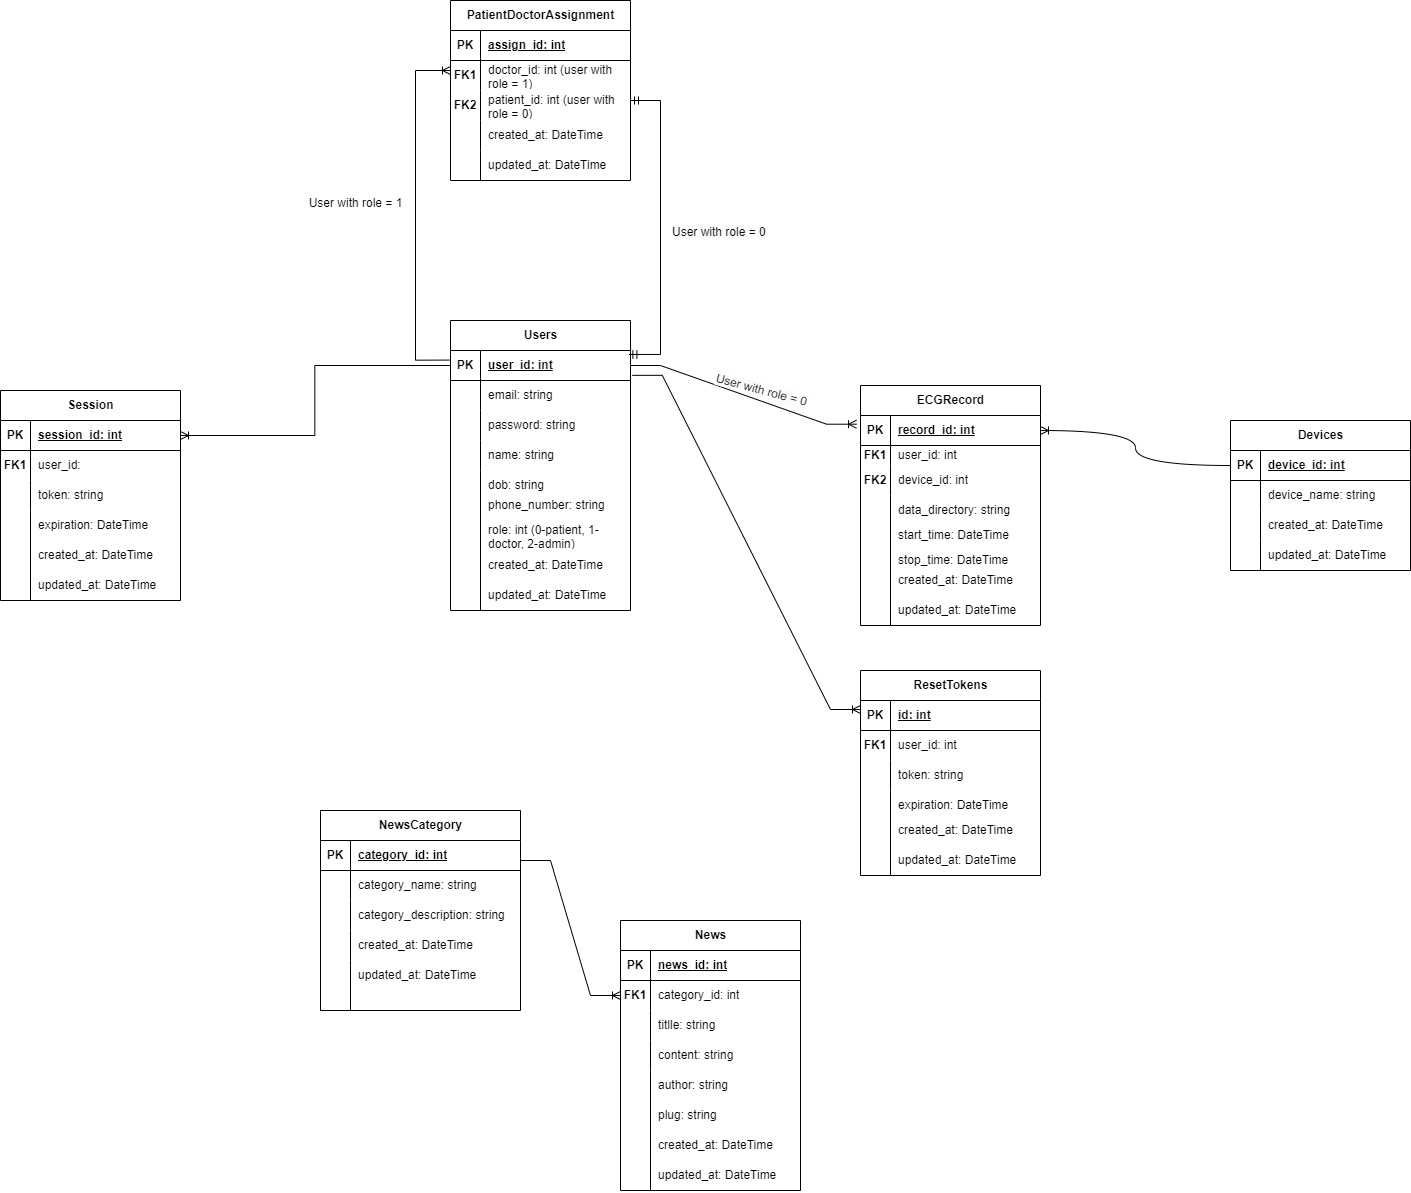
\includegraphics[width=15cm,height=15cm]{Images/server/database/fmECG_architecture-Database.drawio.png}
  \caption[Sơ đồ ERD]{\bfseries \fontsize{12pt}{0pt}\selectfont Sơ đồ ERD}
  \label{fmECG_architecture-Database} %đặt tên cho ảnh
\end{figure}


\subsection{Thiết kế chi tiết hệ thống}



\subsubsection{Thiết kế giao diện}

\paragraph{Ứng dụng}
\mbox{}

Dưới đây là các giao diện thực tế mà chúng em thiết kế cho App:
\begin{figure}[H]
  \centering
  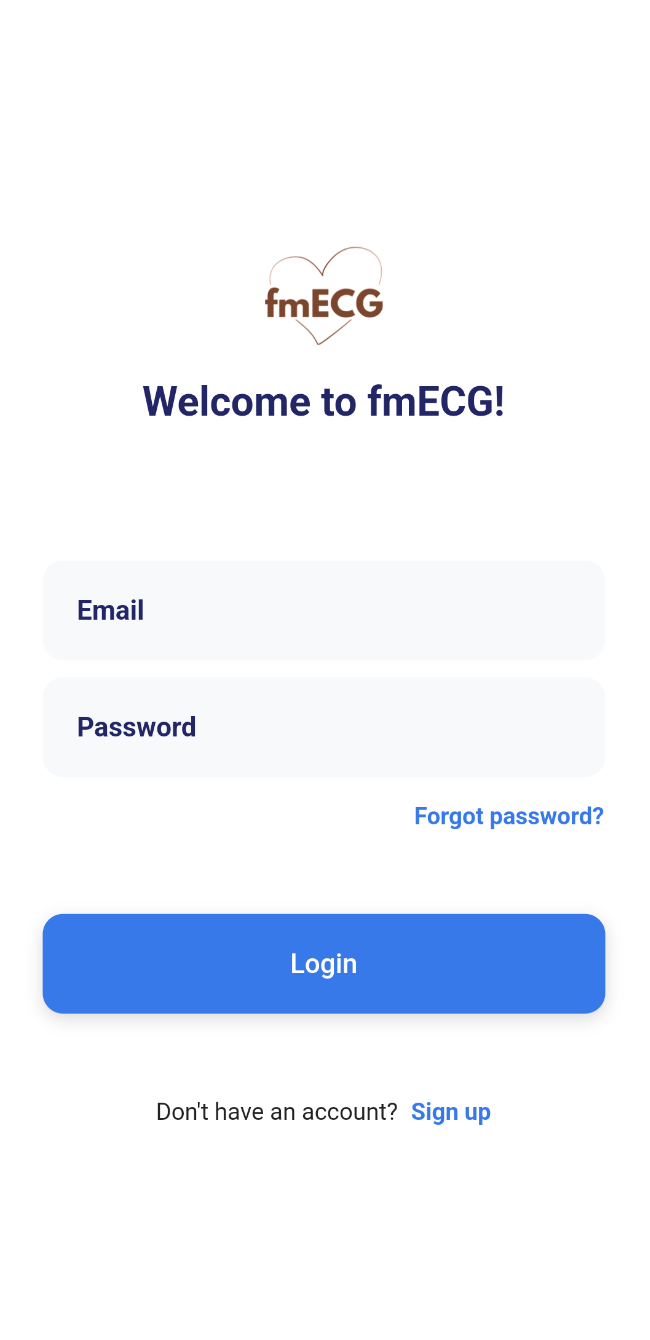
\includegraphics[width=6cm,height=12cm]{Images/mobile_app/demo/login.png}
  \caption[Giao diện trang đăng nhập]{\bfseries \fontsize{12pt}{0pt}\selectfont Giao diện trang đăng nhập}
  \label{demo_login} %đặt tên cho ảnh
\end{figure}

Trang đăng nhập gồm có logo, sau đó là hai ô để nhập email và mật khẩu, cùng một nút màu xanh cho người dùng nhấn để kiểm tra 
việc đăng nhập vào
trang chủ nếu email và mật khẩu của người dùng được xác thực. Nếu việc xác thực không thành công, giao diện sẽ hiển thị
một dòng chữ dưới hai ô nhập.

Ngoài ra nếu người dùng chưa có tài khoản thì có thể chọn đăng ký ở dưới để chuyển sang trang đăng ký.

\begin{figure}[H]
  \centering
  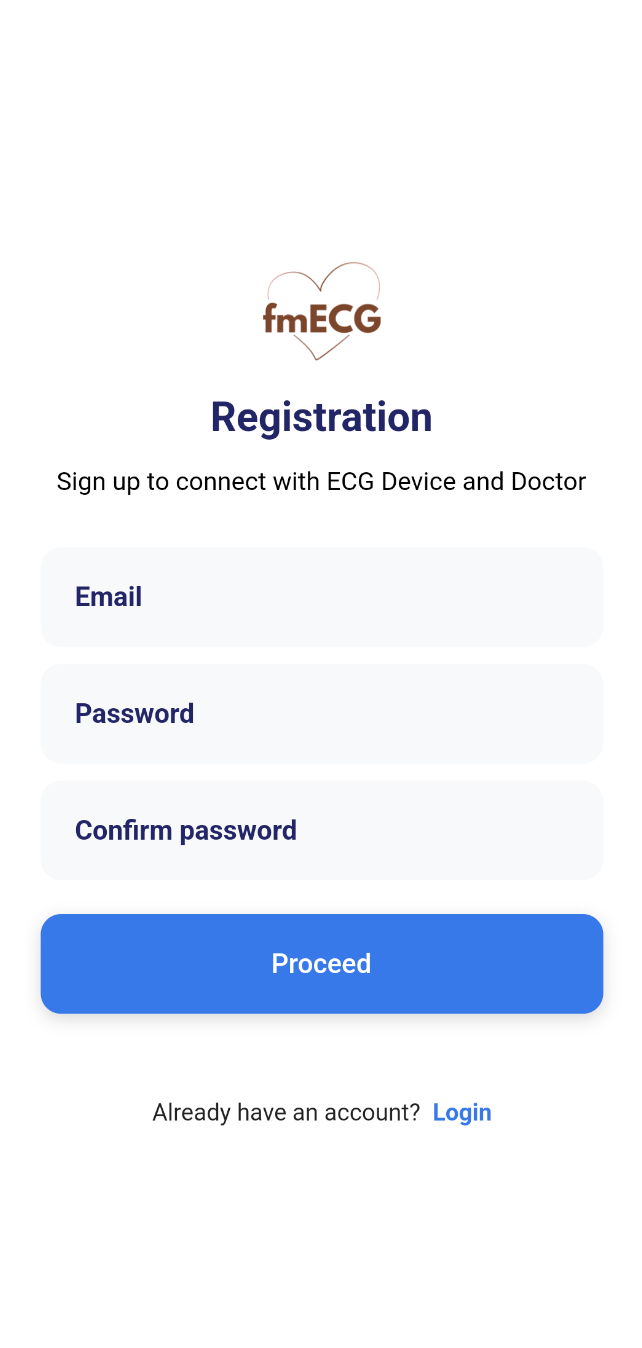
\includegraphics[width=6cm,height=12cm]{Images/mobile_app/demo/register.png}
  \caption[Giao diện trang đăng ký tài khoản]{\bfseries \fontsize{12pt}{0pt}\selectfont Giao diện trang đăng ký tài khoản}
  \label{demo_register} %đặt tên cho ảnh
\end{figure}

Trang đăng ký gồm có 3 ô để người dùng đăng ký tài khoản một cách nhanh chóng

\begin{figure}[H]
  \centering
  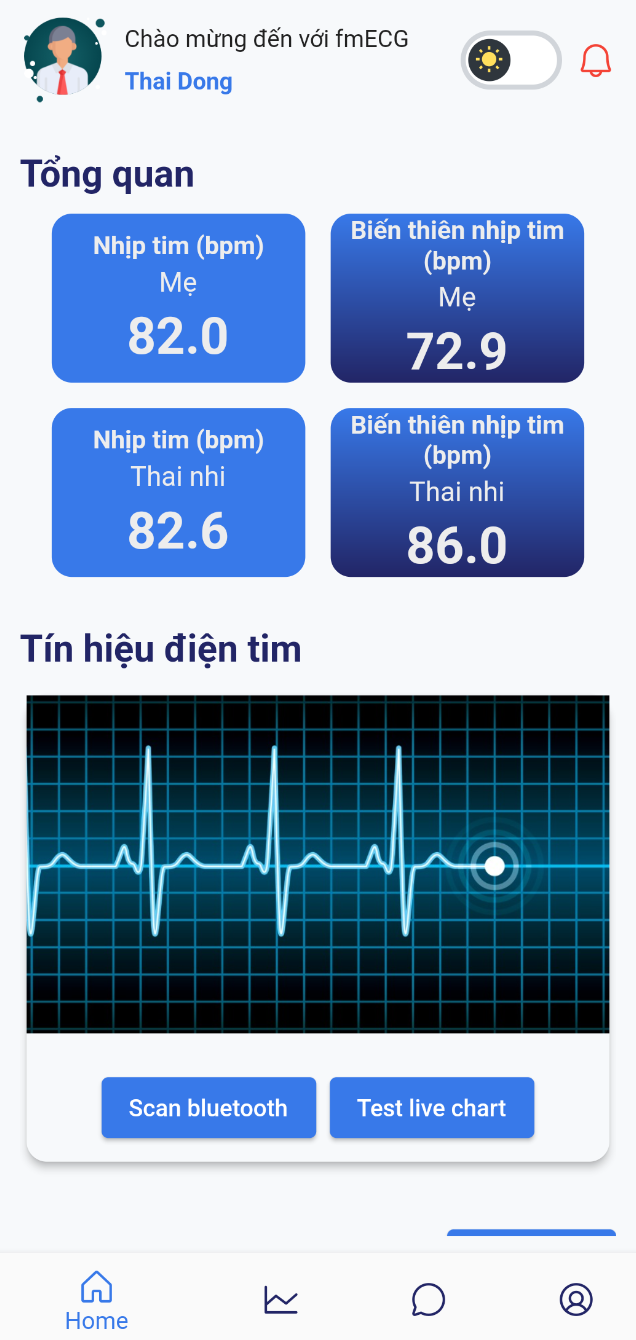
\includegraphics[width=6cm,height=12cm]{Images/mobile_app/demo/home_screen.png}
  \caption[Giao diện trang]{\bfseries \fontsize{12pt}{0pt}\selectfont Giao diện trang}
  \label{demo_} %đặt tên cho ảnh
\end{figure}

\begin{figure}[H]
  \centering
  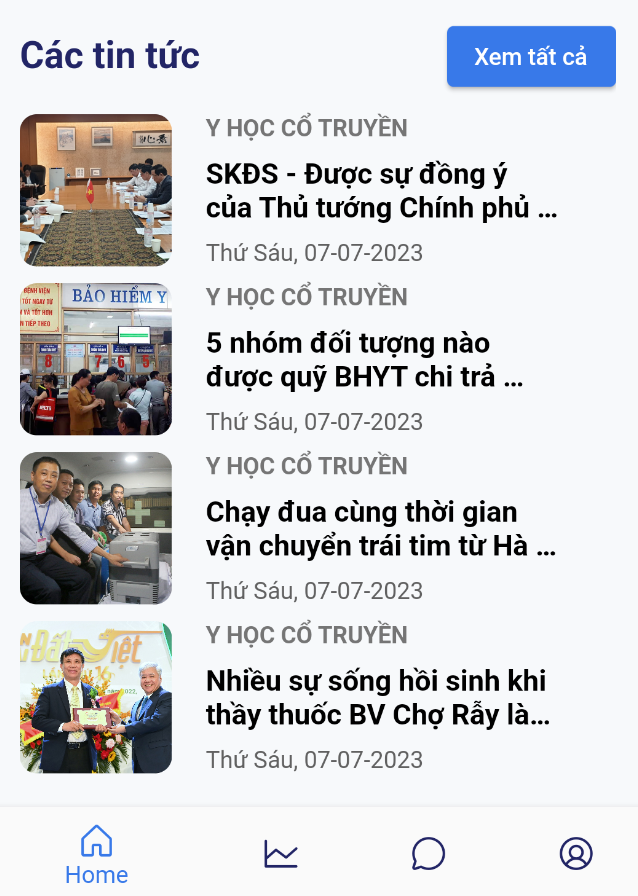
\includegraphics[width=6cm,height=8cm]{Images/mobile_app/demo/preview_news.png}
  \caption[Giao diện trang]{\bfseries \fontsize{12pt}{0pt}\selectfont Giao diện trang}
  \label{demo_} %đặt tên cho ảnh
\end{figure}

\begin{figure}[H]
  \centering
  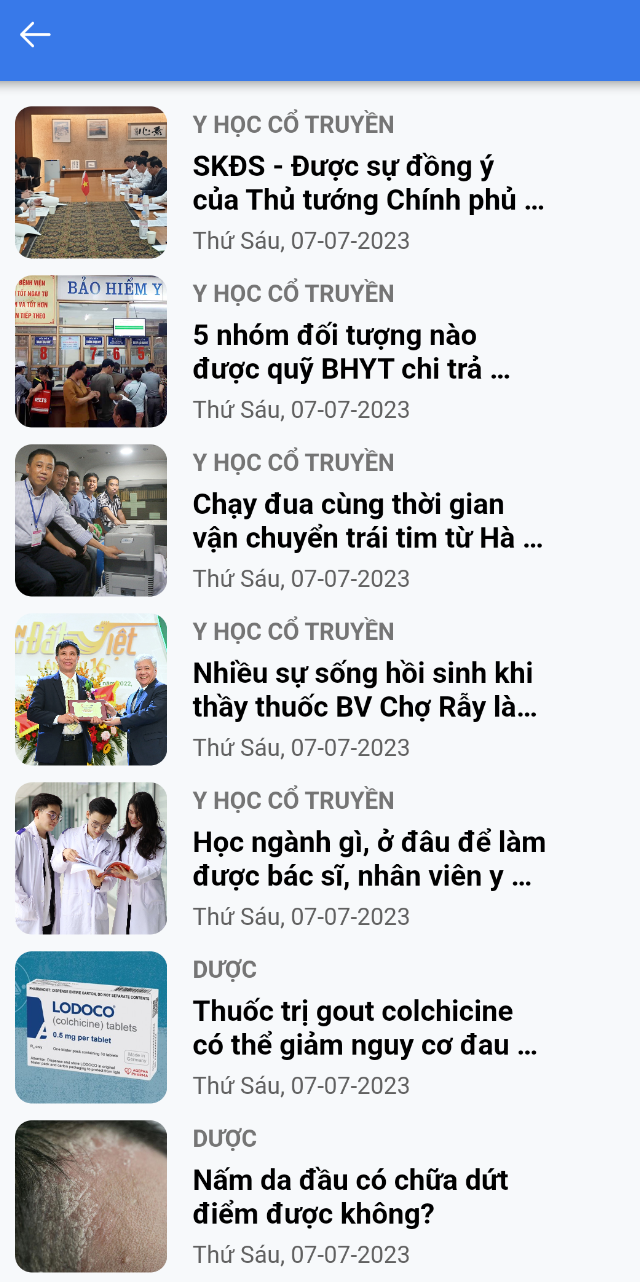
\includegraphics[width=6cm,height=12cm]{Images/mobile_app/demo/all_news.png}
  \caption[Giao diện trang]{\bfseries \fontsize{12pt}{0pt}\selectfont Giao diện trang}
  \label{demo_} %đặt tên cho ảnh
\end{figure}

\begin{figure}[H]
  \centering
  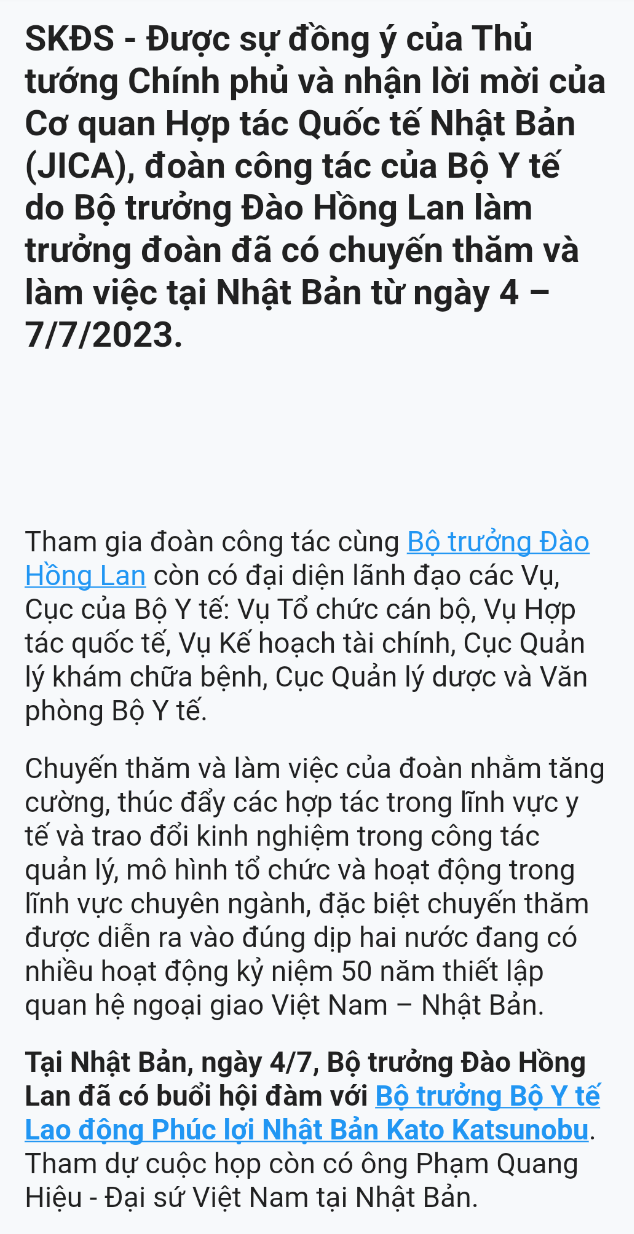
\includegraphics[width=6cm,height=12cm]{Images/mobile_app/demo/detail_news.png}
  \caption[Giao diện trang]{\bfseries \fontsize{12pt}{0pt}\selectfont Giao diện trang}
  \label{demo_} %đặt tên cho ảnh
\end{figure}

\begin{figure}[H]
  \centering
  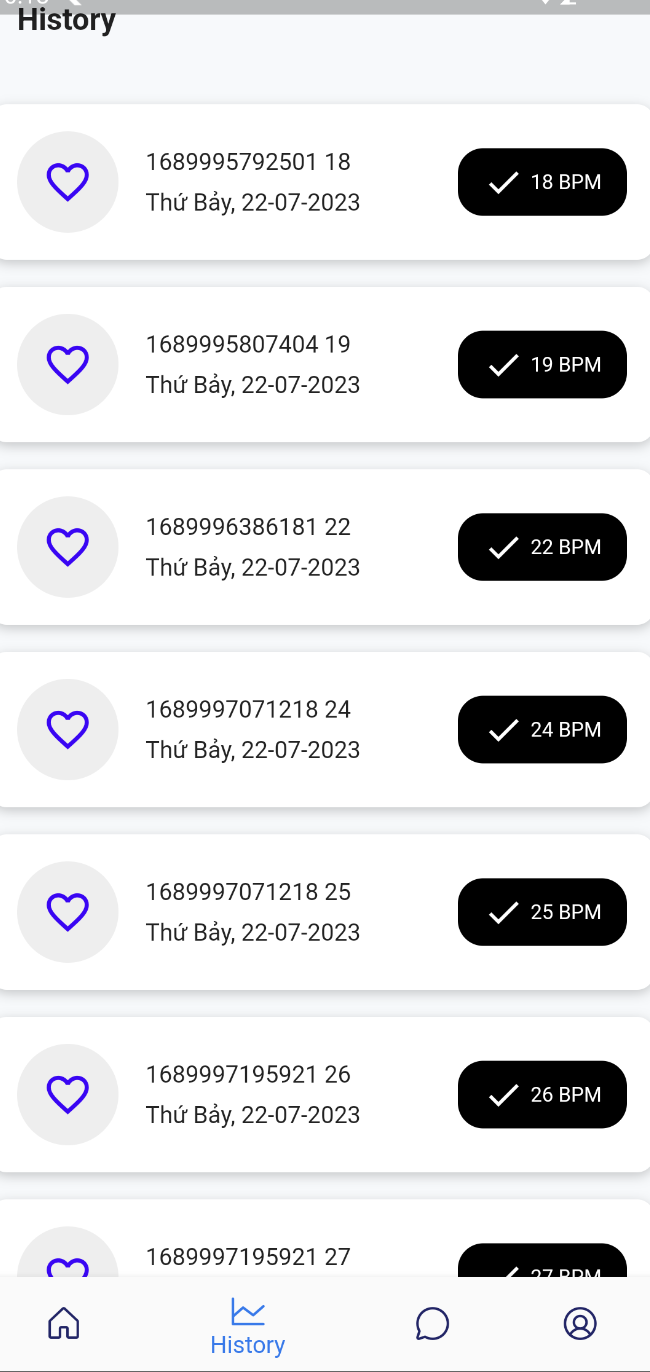
\includegraphics[width=6cm,height=12cm]{Images/mobile_app/demo/history.png}
  \caption[Giao diện trang]{\bfseries \fontsize{12pt}{0pt}\selectfont Giao diện trang}
  \label{demo_} %đặt tên cho ảnh
\end{figure}

\begin{figure}[H]
  \centering
  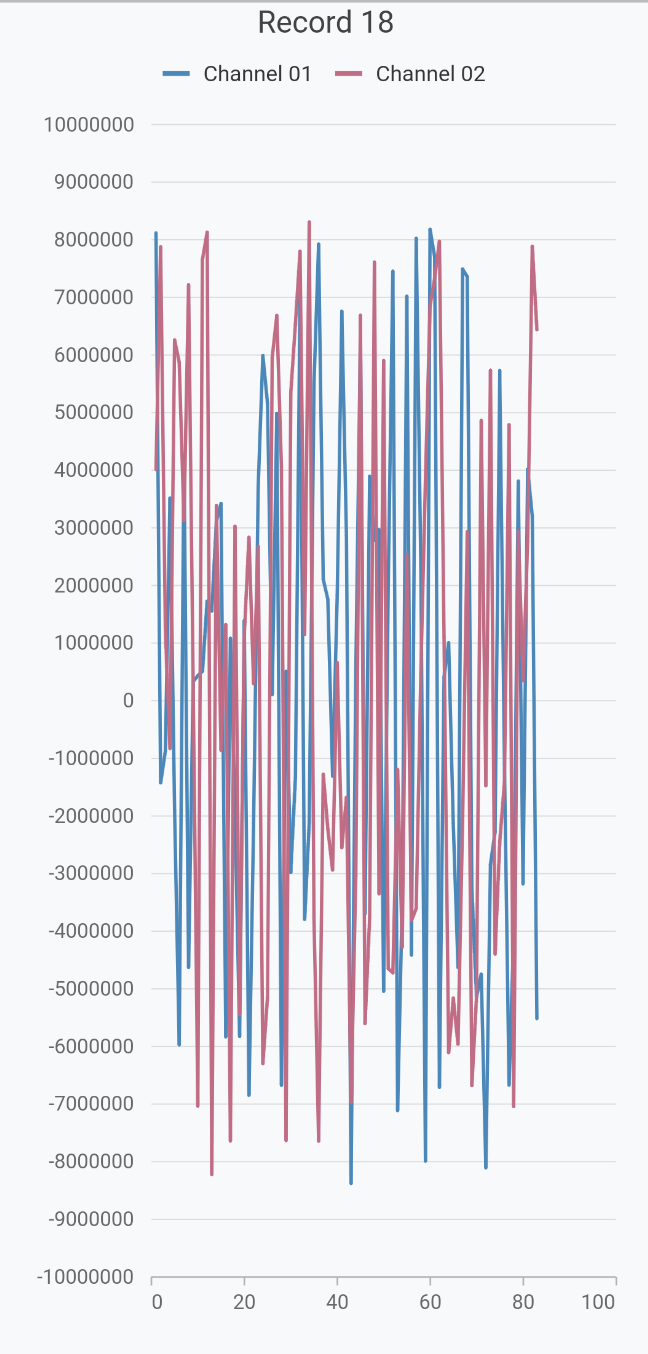
\includegraphics[width=6cm,height=12cm]{Images/mobile_app/demo/detail_record.png}
  \caption[Giao diện trang]{\bfseries \fontsize{12pt}{0pt}\selectfont Giao diện trang}
  \label{demo_} %đặt tên cho ảnh
\end{figure}

\begin{figure}[H]
  \centering
  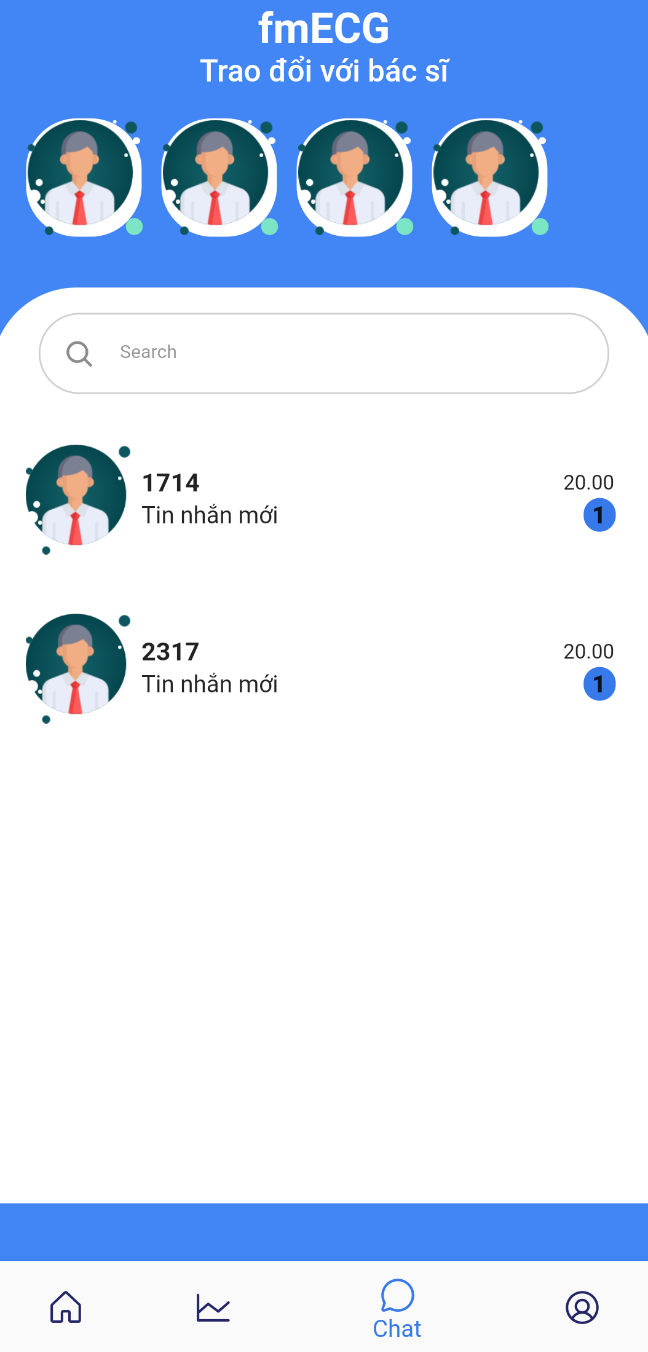
\includegraphics[width=6cm,height=12cm]{Images/mobile_app/demo/chat_preview.png}
  \caption[Giao diện trang]{\bfseries \fontsize{12pt}{0pt}\selectfont Giao diện trang}
  \label{demo_} %đặt tên cho ảnh
\end{figure}

\begin{figure}[H]
  \centering
  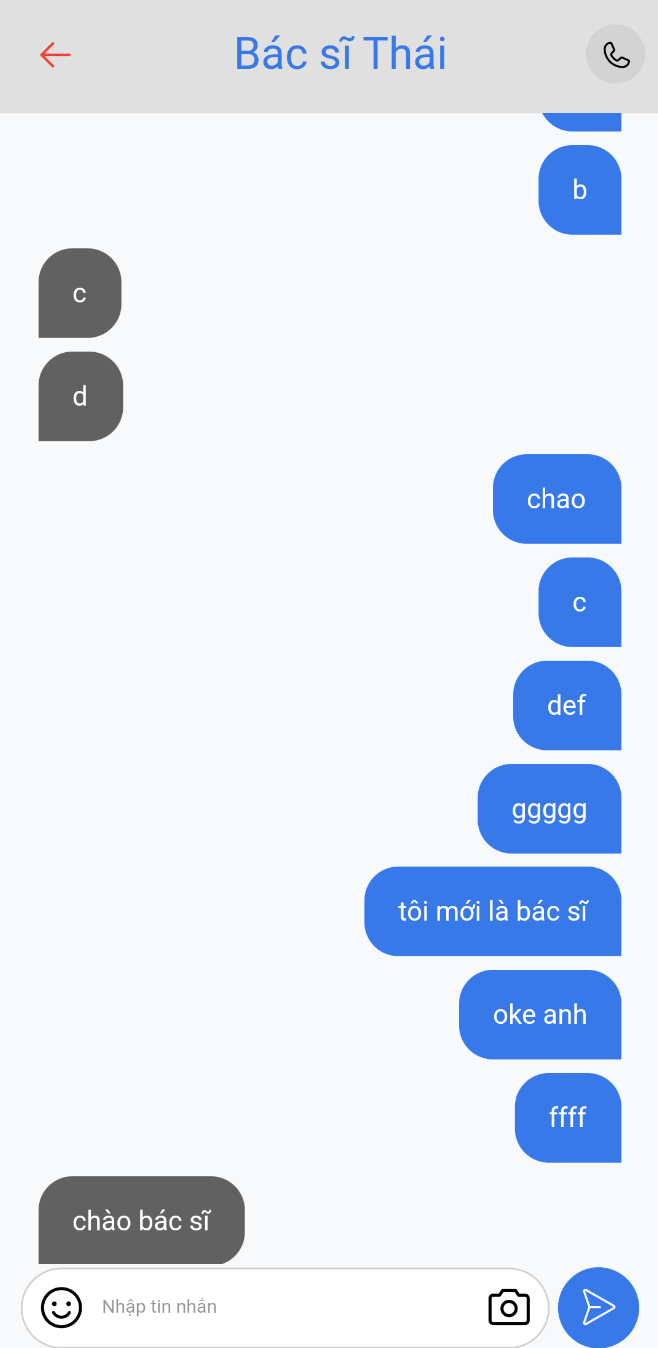
\includegraphics[width=6cm,height=12cm]{Images/mobile_app/demo/chat_detail.png}
  \caption[Giao diện trang]{\bfseries \fontsize{12pt}{0pt}\selectfont Giao diện trang}
  \label{demo_} %đặt tên cho ảnh
\end{figure}

\begin{figure}[H]
  \centering
  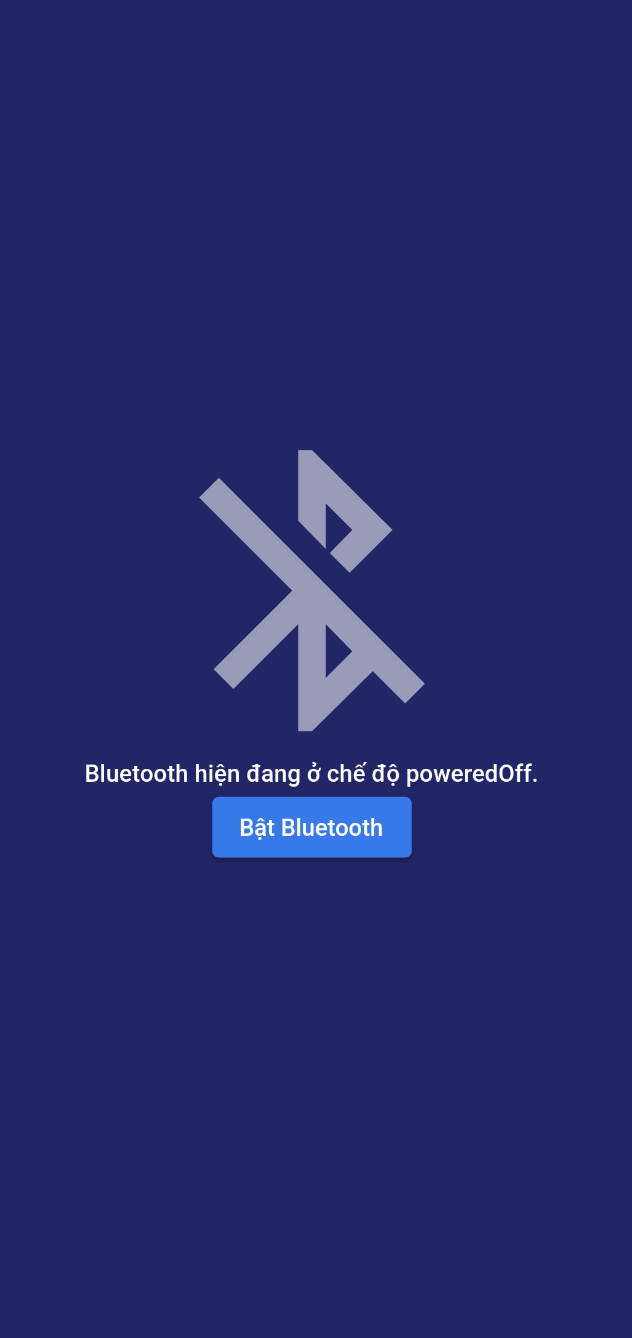
\includegraphics[width=6cm,height=12cm]{Images/mobile_app/demo/off_bluetooth.png}
  \caption[Giao diện trang]{\bfseries \fontsize{12pt}{0pt}\selectfont Giao diện trang}
  \label{demo_} %đặt tên cho ảnh
\end{figure}


\begin{figure}[H]
  \centering
  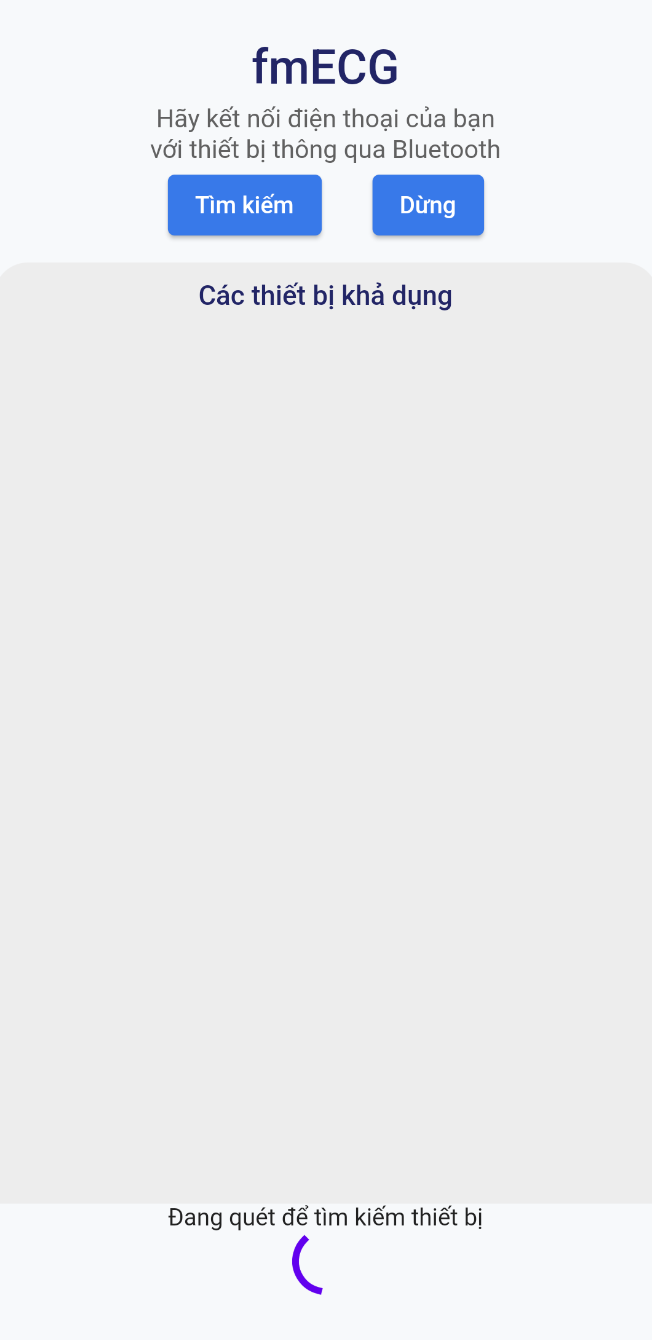
\includegraphics[width=6cm,height=12cm]{Images/mobile_app/demo/finding_bluetooth.png}
  \caption[Giao diện trang]{\bfseries \fontsize{12pt}{0pt}\selectfont Giao diện trang}
  \label{demo_} %đặt tên cho ảnh
\end{figure}



\paragraph{Website}
\mbox{}



\begin{figure}[H]
  \centering
  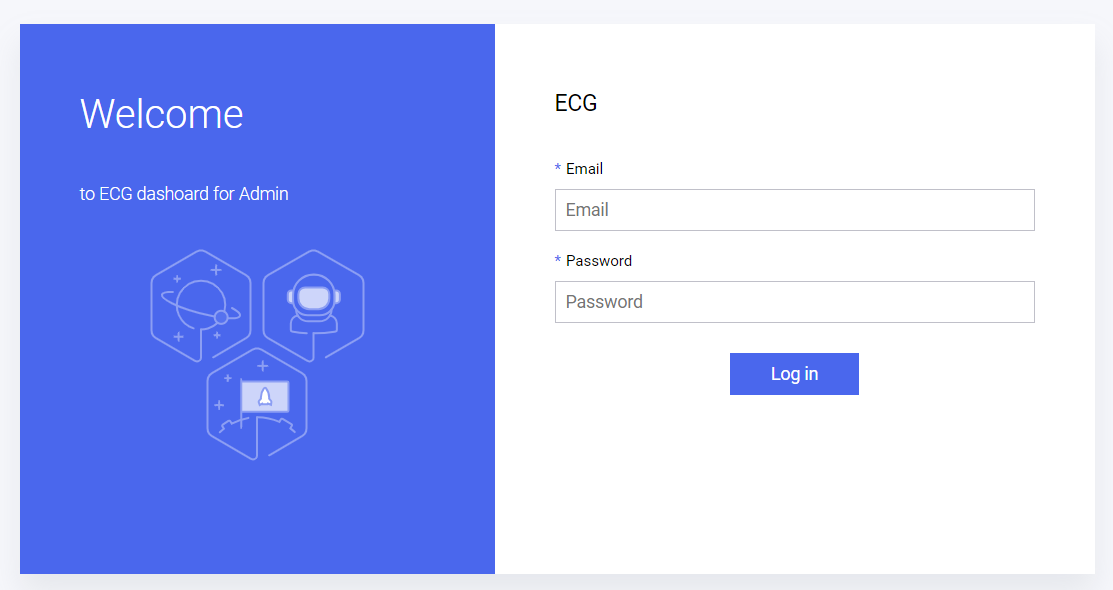
\includegraphics[scale=0.7]{Images/server/webUI/login.PNG}
  \caption[Giao diện trang]{\bfseries \fontsize{12pt}{0pt}\selectfont Giao diện trang}
  \label{demo_} %đặt tên cho ảnh
\end{figure}

\begin{figure}[H]
  \centering
  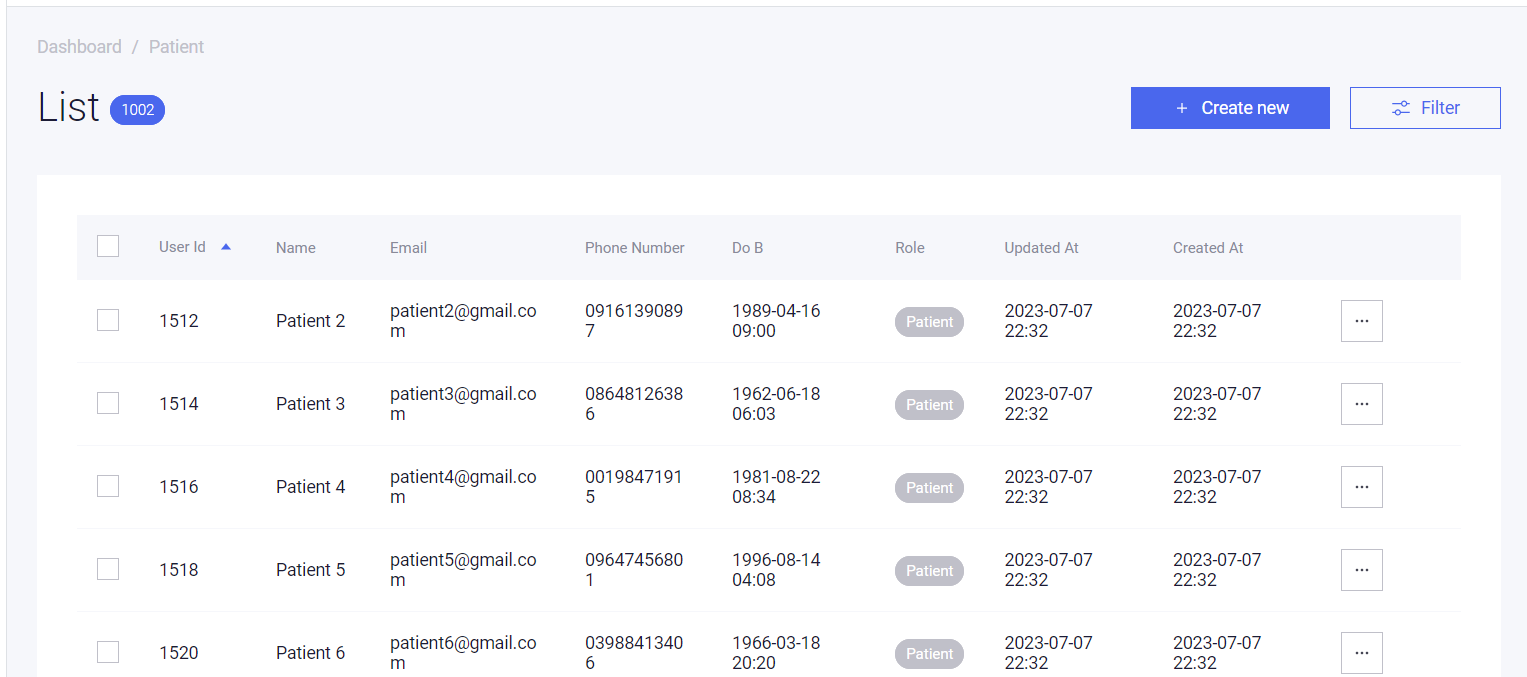
\includegraphics[scale=0.5]{Images/server/webUI/patient_list.PNG}
  \caption[Giao diện trang]{\bfseries \fontsize{12pt}{0pt}\selectfont Giao diện trang}
  \label{demo_} %đặt tên cho ảnh
\end{figure}


\begin{figure}[H]
  \centering
  \includegraphics[scale=0.5]{Images/server/webUI/list_doctor.PNG}
  \caption[Giao diện trang]{\bfseries \fontsize{12pt}{0pt}\selectfont Giao diện trang}
  \label{demo_} %đặt tên cho ảnh
\end{figure}


\begin{figure}[H]
  \centering
  \includegraphics[scale=0.5]{Images/server/webUI/news_list.PNG}
  \caption[Giao diện trang]{\bfseries \fontsize{12pt}{0pt}\selectfont Giao diện trang}
  \label{demo_} %đặt tên cho ảnh
\end{figure}

\begin{figure}[H]
  \centering
  \includegraphics[scale=0.5]{Images/server/webUI/news_category_list.PNG}
  \caption[Giao diện trang]{\bfseries \fontsize{12pt}{0pt}\selectfont Giao diện trang}
  \label{demo_} %đặt tên cho ảnh
\end{figure}


\begin{figure}[H]
  \centering
  \includegraphics[scale=0.5]{Images/server/webUI/ecg_record_list.PNG}
  \caption[Giao diện trang]{\bfseries \fontsize{12pt}{0pt}\selectfont Giao diện trang}
  \label{demo_} %đặt tên cho ảnh
\end{figure}


\begin{figure}[H]
  \centering
  \includegraphics[scale=0.5]{Images/server/webUI/pat_doc_list.PNG}
  \caption[Giao diện trang]{\bfseries \fontsize{12pt}{0pt}\selectfont Giao diện trang}
  \label{demo_} %đặt tên cho ảnh
\end{figure}

\subsubsection{Sơ đồ lớp cho ứng dụng di động, website và server}

\paragraph{Ứng dụng di động}
\mbox{}

Ứng dụng di động được tổ chức theo mô hình MVC, với ba khối chính là Models, Views và Controllers:
  
\begin{itemize}
  \item Khối "Models": Chứa các lớp đại diện cho các đối tượng của cơ sở dữ liệu, định nghĩa các thuộc tính và phương thức để làm việc với dữ liệu.
 
  \item Khối "Controllers": Chứa các controllers xử lý logic và điều khiển các yêu cầu từ người dùng.

  \item Khối "Views": Chứa các lớp route, xác định các endpoint và xử lý các yêu cầu HTTP từ người dùng bằng cách gọi tới các controllers tương ứng.
\end{itemize}

Chi tiết từng lớp và phần giải thích cho mỗi khối được chúng em thể hiện bằng hình và lời trong các mục bên dưới. 

\begin{enumerate}[a)]
  \item Danh sách các class diagram cho ứng dụng di động
    
  \begin{figure}[H]
    \centering
    \includegraphics[width=16cm,height=18cm]{Images/mobile_app/class_diagram/mobile_class_model.png}
    \caption[Sơ đồ lớp của khối Models trong ứng dụng di động]{\bfseries \fontsize{12pt}{0pt}\selectfont Sơ đồ lớp của khối Models trong ứng dụng di động}
    \label{mobile_class_model} %đặt tên cho ảnh
  \end{figure}

  Dựa trên mục \ref{design_database} về phần thiết kế cơ sở dữ liệu, Hình \ref{mobile_class_model} thể hiện các lớp trong Models:
  \begin{itemize}
    \item ECGRecordModel: Lớp thể hiện cấu trúc của một bản ghi dữ liệu điện tim
    \item NewsModel: Lớp thể hiện cấu trúc một tin tức
    \item NewsCategoryModel: Lớp thể hiện cấu trúc một danh mục tin tức
    \item UserModel: Lớp thể hiện cho cấu trúc người dùng trong hệ thống
    \item DeviceModel: Lớp thể hiện cho thông tin thiết bị điện tim 
    \item PatientDoctorAssignmentModel: Lớp thể hiện cho thông tin phân công bác sĩ và bệnh nhân.
  \end{itemize}

  Mỗi lớp đều có một hàm fromJSON để chuyển từ dữ liệu JSON lấy từ API vào trong Model tương ứng. Điều này giúp
  việc code và xử lý trở nên dễ dàng hơn. Sau khi định nghĩa được các Model.
  
  Phần tiếp theo là xác định các Views hay giao diện cần có trong ứng dụng di động và Controllers xử lý logic với những
  yêu cầu từ người dùng.

  \begin{figure}[H]
    \centering
    \includegraphics[width=14cm,height=7cm]{Images/mobile_app/class_diagram/mobile_class_view.png}
    \caption[Sơ đồ lớp của khối Views trong ứng dụng di động]{\bfseries \fontsize{12pt}{0pt}\selectfont Sơ đồ lớp của khối Views trong ứng dụng di động}
    \label{mobile_class_view} %đặt tên cho ảnh
  \end{figure}

  Hình \ref{mobile_class_view} thể hiện các lớp trong Views. Mỗi use case liên quan đến bệnh nhân/bác sĩ thể hiện ở sơ đồ 
  usecase Hình \ref{use_case_general} sẽ đại diện cho một lớp giao diện tương ứng. Trong đó sẽ gồm các màn cho từng chức năng
  cụ thể:

  \begin{itemize}
    \item MainScreens: Các giao diện không thuộc chức năng cụ thể, những giao diện chính là tiền đề cho các giao diện chức năng khác
    \item AuthScreens: Các giao diện xác thực người dùng 
    \item BluetoothScreens: Các giao diện phục vụ cho quá trình kết nối và theo dõi dữ liệu điện tim thông qua bluetooth
    \item NewsScreens: Các giao diện xem tin tức
    \item UserScreens: Các giao diện cho người dùng
    \item ChatScreens: Các giao diện phục vụ quá trình trao đổi giữa bác sĩ và bệnh nhân
    \item HistoryRecordsScreens: Các giao diện cho phép người dùng xem lại lịch sử đo cùng với biểu đồ. 
  \end{itemize}
  
  \begin{figure}[H]
    \centering
    \includegraphics[width=16cm,height=15cm]{Images/mobile_app/class_diagram/mobile_class_controller.png}
    \caption[Sơ đồ lớp của khối Controllers trong ứng dụng di động]{\bfseries \fontsize{12pt}{0pt}\selectfont Sơ đồ lớp của khối Controllers trong ứng dụng di động}
    \label{mobile_class_controller} %đặt tên cho ảnh
  \end{figure}

  Hình \ref{mobile_class_controller} thể hiện các lớp trong Controllers. Mỗi lớp trong Controllers quản lý một nhiệm vụ
  nhất định được chia nhỏ thành các hàm, phương thức tương ứng giúp việc phia chia và đặc biệt khi kiểm soát lỗi rất dễ dàng do
  chúng ta có thể dự đoán được lỗi phát sinh ở chức năng và hàm nào. 

  % //TODO: Thiếu file managements trong sơ đồ
  \begin{itemize}
    \item AuthProvider: Cung cấp các biến và hàm để thực hiện chức năng xác thực người dùng
    \item ECGRecordController: Cung cấp các hàm, phương thức để thực hiện chức năng liên quan đến các bản ghi điện tim
    \item ECGDataController: Cung cấp các hàm, phương thức để xử lý dữ liệu của bản ghi diện tim thời gian thực
    \item FileController: Cung cấp các hàm, phương thức để xử lý file (tạo, sửa, xoá file), phục vụ chính cho ECGRecordController  
    \item NewsController: Cung cấp các hàm, phương thức để lấy dữ liệu tin tức
    \item PatientDoctorAssignmentController: Cung cấp các hàm, phương thức để lấy dữ liệu phân công bệnh nhân/bác sĩ
    \item UserController: Cung cấp các hàm, phương thức để thao tác với dữ liệu người dùng 
    \item FirebaseMessagesController: Cung cấp các hàm, phương thức để thao tác với tin nhắn.
  \end{itemize}

  Các lớp được hình thành là nền tảng để viết code dễ dàng hơn, đồng thời điều này cũng giúp cho cấu trúc thư mục trong
  bất kỳ dự án nào trở nên sạch sẽ và dễ theo dõi hơn.
  
  \end{enumerate}

\paragraph{Server và Website quản trị hệ thống}
\mbox{}

\begin{enumerate}[a)]
\item Danh sách các class diagram

\begin{figure}[H]
  \centering
  \includegraphics[width=16cm,height=13cm]{Images/server/class/class_controller.png}
  \caption[Sơ đồ lớp của package Controllers]{\bfseries \fontsize{12pt}{0pt}\selectfont Sơ đồ lớp của package Controllers}
  \label{class_controller} %đặt tên cho ảnh
\end{figure}



\begin{figure}[H]
  \centering
  \includegraphics[width=15cm,height=16cm]{Images/server/class/class_model.png}
  \caption[Sơ đồ lớp của package Models]{\bfseries \fontsize{12pt}{0pt}\selectfont Sơ đồ lớp của package Models}
  \label{class_model} %đặt tên cho ảnh
\end{figure}


\begin{figure}[H]
  \centering
  \includegraphics[width=14cm,height=6cm]{Images/server/class/class_route.png}
  \caption[Sơ đồ lớp của package Routes]{\bfseries \fontsize{12pt}{0pt}\selectfont Sơ đồ lớp của package Routes}
  \label{class_route} %đặt tên cho ảnh
\end{figure}


\begin{figure}[H]
  \centering
  \includegraphics[width=15cm,height=14cm]{Images/server/class/class_admin.png}
  \caption[Sơ đồ lớp của package View và Admin]{\bfseries \fontsize{12pt}{0pt}\selectfont Sơ đồ lớp của package View và Admin}
  \label{class_admin} %đặt tên cho ảnh
\end{figure}


\begin{itemize}

  \item Package "Controllers":

  Chứa các controllers xử lý logic và điều khiển các yêu cầu từ người dùng.
  \item Package "Models":
  
  Chứa các lớp đại diện cho các đối tượng của cơ sở dữ liệu, định nghĩa các thuộc tính và phương thức để làm việc với dữ liệu.
  \item Package "Routes":
  
  Chứa các lớp route, xác định các endpoint và xử lý các yêu cầu HTTP từ người dùng bằng cách gọi tới các controllers tương ứng.
  \item Package "Views":
  
  Chứa các view components đại diện cho giao diện người dùng.
  \item Package "Admin":
  
  Chứa các thành phần liên quan đến trang Admin dashboard.
  \item Package "Resources" (Trong "Admin"):
  
  Chứa các lớp Resource (nguồn tài nguyên) đại diện cho các tài nguyên của trang Admin dashboard, bao gồm: AdminResource, DoctorResource, PatientResource, ECGRecordResource, NewsResource, NewsCategoryResource và PatientDoctorAssignmentResource.
  \item Package "Components" (Trong "Admin"):
  
  Chứa các lớp Components đại diện cho các thành phần giao diện của trang Admin dashboard, bao gồm: ComponentLoader, DashboardViewComponent, NewsViewComponent, ECGRecordViewComponent và PatientDoctorAssignmentViewComponent.
\end{itemize}



\item Mối quan hệ

\begin{figure}[H]
  \centering
  \includegraphics[width=15cm,height=12cm]{Images/server/class/class_relation.png}
  \caption[Mối quan hệ giữa các class ở phía server]{\bfseries \fontsize{12pt}{0pt}\selectfont Mối quan hệ giữa các class ở phía server}
  \label{class_relation} %đặt tên cho ảnh
\end{figure}


\begin{figure}[H]
  \centering
  \includegraphics[width=16cm,height=15cm]{Images/server/class/class_admin_relation.png}
  \caption[Mối quan hệ giữa các class ở phía website quản trị]{\bfseries \fontsize{12pt}{0pt}\selectfont Mối quan hệ giữa các class ở phía website quản trị}
  \label{class_admin_relation} %đặt tên cho ảnh
\end{figure}

\end{enumerate}



\subsubsection{Thiết kế các chức năng cho Website và Server}

\paragraph{Thiết kế API}
\mbox{}

\begin{enumerate}[a)]
  \item API liên quan đến thông tin người dùng
  

  \begin{table}[H]
    \centering
    \caption{\bfseries \fontsize{12pt}{0pt}\selectfont Bảng API liên quan đến thông tin người dùng}
    \begin{tabularx}{0.9\textwidth}{
    | >{\raggedright\arraybackslash}X
    | >{\raggedright\arraybackslash}m{2cm}
    | >{\raggedright\arraybackslash}X|
    }
    \hline
    \bfseries Đường dẫn    &\bfseries Phương thức    &\bfseries Mô tả\\ \hline
   api/users/profile   &   GET  &  Lấy thông tin của người dùng với đầu vào là JWT token khi người dùng đăng nhập thành công vào hệ thống \\  \hline
   api/users/profile   &    PUT    &  Cập nhật thông tin người dùng \\  \hline
   api/users/change-password   &   PUT     & Thay đổi mật khẩu của người dùng  \\ \hline
   api/users/\{:userId\}  &   GET     & Lấy thông tin của người dùng cụ thể theo user id \\ \hline

    \end{tabularx}
    \label{table_api_user}
\end{table}

\item API liên quan đến việc xác thực người dùng


\begin{table}[H]
  \centering
  \caption{\bfseries \fontsize{12pt}{0pt}\selectfont Bảng API liên quan đến việc xác thực người dùng}
  \begin{tabularx}{0.9\textwidth}{
  | >{\raggedright\arraybackslash}X
  | >{\raggedright\arraybackslash}m{2cm}
  | >{\raggedright\arraybackslash}X|
  }
  \hline
  \bfseries Đường dẫn    &\bfseries Phương thức    &\bfseries Mô tả\\ \hline
 api/register   &   POST  & Đăng ký tài khoản \\ \hline
 api/login   &    POST    & Đăng nhập vào hệ thống \\ \hline
 api/logout  &   GET     & Đăng xuất khỏi hệ thống \\ \hline
 api/reset-password  &     POST   &  Gửi reset token đến email của người dùng để reset mật khẩu \\  \hline
 api/reset-password/reset &   POST     & Giúp reset lại mật khẩu mới với verify token được nhận từ api: api/reset-password  \\ \hline

  \end{tabularx}
  \label{table_api_auth}
\end{table}


\item API liên quan đến tin tức


\begin{table}[H]
  \centering
  \caption{\bfseries \fontsize{12pt}{0pt}\selectfont Bảng API liên quan đến tin tức}
  \begin{tabularx}{0.9\textwidth}{
  | >{\raggedright\arraybackslash}X
  | >{\raggedright\arraybackslash}m{2cm}
  | >{\raggedright\arraybackslash}X|
  }
  \hline
  \bfseries Đường dẫn    &\bfseries Phương thức    &\bfseries Mô tả\\ \hline
 api/news/\{:newsId\}   &   GET  & Lấy nội của tin tức tương ứng với id dưới dạng HTML \\ \hline
 api/news   &    GET    & Lấy toàn bộ danh sách thông tin của tin tức \\ \hline
 api/categories  &   GET     & Lấy toàn bộ danh sách thông tin của tin tức \\ \hline
 api/category/\{:categoryId\}   &     GET   & Lấy thông tin của loại tin tức theo id tương ứng \\ \hline
 api/ news/category/\{:categoryId\} &   GET     & Lấy toàn bộ thông tin của tin tức theo id của loại tin \\ \hline

  \end{tabularx}
  \label{table_api_news}
\end{table}

\item API liên quan đến bản ghi ECG


\begin{table}[H]
  \centering
  \caption{\bfseries \fontsize{12pt}{0pt}\selectfont Bảng API liên quan đến bản ghi ECG}
  \begin{tabularx}{0.9\textwidth}{
  | >{\raggedright\arraybackslash}X
  | >{\raggedright\arraybackslash}m{2cm}
  | >{\raggedright\arraybackslash}X|
  }
  \hline
  \bfseries Đường dẫn    &\bfseries Phương thức    &\bfseries Mô tả\\ \hline
 api/ecg-records/upload   &   POST  & Tải dữ liệu của phiên đo ECG lên server \\ \hline
 api/ecg-records/patient/\{:patientId\}   &    GET    & Lấy danh sách thông tin các phiên đo ECG của bệnh nhân \\ \hline
 api/ecg-records/doctor/\{:doctorId\} &   GET     & Lấy danh sách thông tin các phiên đo ECG của các bệnh nhân được quản lý bởi bác sỹ \\ \hline
 api/ecg-records/record-data/\{:recordId\}  &     GET   & Lấy dữ liệu một phiên đo của bệnh nhân \\ \hline

  \end{tabularx}
  \label{table_api_ecg}
\end{table}


\item API liên quan liên quan đến việc phân công bệnh nhân cho bác sỹ



\begin{table}[H]
  \centering
  \caption{\bfseries \fontsize{12pt}{0pt}\selectfont Bảng API liên quan liên quan đến việc phân công bệnh nhân cho bác sỹ}
  \begin{tabularx}{0.9\textwidth}{
  | >{\raggedright\arraybackslash}X
  | >{\raggedright\arraybackslash}m{2cm}
  | >{\raggedright\arraybackslash}X|
  }
  \hline
  \bfseries Đường dẫn    &\bfseries Phương thức    &\bfseries Mô tả\\ \hline
   api/doctor/\{:doctorId\}/patients   &   GET  & Lấy danh sách thông tin bệnh nhân được phân công cho bác sĩ \\ \hline
  api/patient/\{:patientId\}/doctor  &    GET    & Lấy thông tin bác sỹ được phân công cho bệnh nhân \\ \hline

  \end{tabularx}
  \label{table_api_pat_doc}
\end{table}



\end{enumerate}




\paragraph{Sơ đồ tuần tự}
\mbox{}

\begin{enumerate}[a)]

% ------------------------User----------------------

\item  API liên quan đến thông tin người dùng


% sửa lại ảnh 
\begin{figure}[H]
  \centering
  \includegraphics[width=16cm,height=9cm]{Images/server/sequence/server/getUserById.png}
  \caption[Sơ đồ tuần tự cho API lấy thông tin của người dùng dựa trên ID ]{\bfseries \fontsize{12pt}{0pt}
  \selectfont Sơ đồ tuần tự cho API lấy thông tin của người dùng dựa trên ID }
  \label{getUserById} %đặt tên cho ảnh
\end{figure}
Hình \ref{getUserById} mô tả quá trình lấy thông tin người dùng dựa trên ID trong ứng dụng. Người dùng gửi yêu cầu lấy thông tin người dùng theo ID, thông qua các tầng của hệ thống, yêu cầu này được xử lý bởi UserController. UserController kiểm tra thông tin và truy vấn UserModel để lấy thông tin người dùng. Nếu người dùng không tồn tại, hệ thống trả về response lỗi, ngược lại, response chứa thông tin người dùng được gửi lại từ UserController tới người dùng.


% sửa lại ảnh 
\begin{figure}[H]
  \centering
  \includegraphics[width=16cm,height=9cm]{Images/server/sequence/server/getUserProfile.png}
  \caption[Sơ đồ tuần tự cho API lấy thông tin của người dùng dựa trên JWT token ]{\bfseries \fontsize{12pt}{0pt}
  \selectfont Sơ đồ tuần tự cho API lấy thông tin của người dùng dựa trên JWT token }
  \label{getUserProfile} %đặt tên cho ảnh
\end{figure}
Hình \ref{getUserProfile} mô tả quá trình lấy thông tin hồ sơ người dùng trong ứng dụng. Người dùng gửi yêu cầu lấy thông tin hồ sơ, thông qua các tầng của hệ thống, yêu cầu này được xử lý bởi UserController. UserController giải mã mã thông báo (token) để xác định người dùng, sau đó truy vấn UserModel để lấy thông tin hồ sơ của người dùng dựa trên user\_id từ mã giải mã. Nếu người dùng không tồn tại, hệ thống trả về response lỗi, ngược lại, response chứa thông tin hồ sơ của người dùng được gửi lại từ UserController tới người dùng.




% \linebreak


\begin{figure}[H]
  \centering
  \includegraphics[width=14cm,height=15cm]{Images/server/sequence/server/changePassword.png}
  \caption[Sơ đồ tuần tự cho API thay đổi mật khẩu người dùng ]{\bfseries \fontsize{12pt}{0pt}
  \selectfont Sơ đồ tuần tự cho API thay đổi mật khẩu người dùng }
  \label{changePassword} %đặt tên cho ảnh
\end{figure}

Hình \ref{changePassword} mô tả quá trình thay đổi mật khẩu người dùng trong ứng dụng. Người dùng gửi yêu cầu thay đổi mật khẩu, thông qua các tầng của hệ thống, yêu cầu này được xử lý bởi UserController. Đầu tiên, hệ thống sẽ kiểm tra và giải mã mã thông báo (token) để xác định người dùng. Sau đó, UserController truy vấn UserModel để tìm người dùng dựa trên user\_id từ mã giải mã. Nếu người dùng không tồn tại hoặc mật khẩu hiện tại không khớp với mật khẩu trong hệ thống, hoặc mật khẩu mới không khớp với xác nhận mật khẩu, hệ thống sẽ trả về response lỗi tương ứng. Ngược lại, mật khẩu mới sẽ được mã hóa và lưu vào UserModel, sau đó hệ thống trả về response thành công tới người dùng.



\begin{figure}[H]
  \centering
  \includegraphics[width=16cm,height=12cm]{Images/server/sequence/server/updateUserInfo.png}
  \caption[Sơ đồ tuần tự cho API cập nhật thông tin người dùng ]{\bfseries \fontsize{12pt}{0pt}
  \selectfont Sơ đồ tuần tự cho API cập nhật thông tin người dùng }
  \label{updateUserInfo} %đặt tên cho ảnh
\end{figure}

Hình \ref{updateUserInfo} mô tả quá trình cập nhật thông tin người dùng trong ứng dụng. Người dùng gửi yêu cầu cập nhật thông tin, thông qua các tầng của hệ thống, yêu cầu này được xử lý bởi UserController. Đầu tiên, hệ thống sẽ kiểm tra và giải mã mã thông báo (token) để xác định người dùng. Sau đó, UserController truy vấn UserModel để tìm người dùng dựa trên user\_id từ mã giải mã. Nếu người dùng không tồn tại, hệ thống sẽ trả về response lỗi. Ngược lại, thông tin cập nhật như tên, ngày sinh (dob), và số điện thoại (phone\_number) sẽ được cập nhật vào UserModel. Sau đó, hệ thống trả về response thành công tới người dùng.


% ----------------------------------------------



% ------------------------Auth----------------------

\item API liên quan đến việc xác thực người dùng 

\begin{figure}[H]
  \centering
  \includegraphics[width=16cm,height=12cm]{Images/server/sequence/server/login.png}
  \caption[Sơ đồ tuần tự cho API đăng nhập vào hệ thống]{\bfseries \fontsize{12pt}{0pt}
  \selectfont Sơ đồ tuần tự cho API đăng nhập vào hệ thống }
  \label{backend_login} %đặt tên cho ảnh
\end{figure}
Hình \ref{backend_login}  mô tả quá trình xác thực người dùng đăng nhập vào ứng dụng. Người dùng gửi yêu cầu đăng nhập, thông qua các tầng của hệ thống, yêu cầu này được xử lý bởi AuthController. AuthController kiểm tra thông tin người dùng, tạo token nếu đúng thông tin đăng nhập và trả về response cho người dùng.

\begin{figure}[H]
  \centering
  \includegraphics[width=16cm,height=9cm]{Images/server/sequence/server/logout.png}
  \caption[Sơ đồ tuần tự cho API đăng xuất khỏi hệ thống ]{\bfseries \fontsize{12pt}{0pt}
  \selectfont Sơ đồ tuần tự cho API đăng xuất khỏi hệ thống }
  \label{backend_logout} %đặt tên cho ảnh
\end{figure}
Hình \ref{backend_logout} mô tả quá trình đăng xuất (logout) người dùng khỏi ứng dụng. Người dùng gửi yêu cầu đăng xuất, thông qua các tầng của hệ thống, yêu cầu này được xử lý bởi AuthController. Đầu tiên, hệ thống kiểm tra xem cookie token có tồn tại hay không. Nếu không tồn tại, hệ thống trả về response lỗi. Ngược lại, AuthController xóa cookie và gọi tới SessionModel để hủy phiên đăng nhập của người dùng dựa trên token trong cookie. Sau khi xử lý, hệ thống trả về response thành công tới người dùng.

\begin{figure}[H]
  \centering
  \includegraphics[width=16cm,height=12cm]{Images/server/sequence/server/register.png}
  \caption[Sơ đồ tuần tự cho API đăng ký tài khoản]{\bfseries \fontsize{12pt}{0pt}
  \selectfont Sơ đồ tuần tự cho API đăng ký tài khoản }
  \label{backend_register} %đặt tên cho ảnh
\end{figure}
Hình \ref{backend_register} mô tả quá trình đăng ký tài khoản trong ứng dụng. Người dùng gửi yêu cầu đăng ký, thông qua các tầng của hệ thống, yêu cầu này được xử lý bởi AuthController. Đầu tiên, hệ thống kiểm tra thông tin yêu cầu đăng ký, bao gồm việc kiểm tra mật khẩu và xác nhận mật khẩu có khớp hay không. Sau đó, AuthController kiểm tra xem người dùng đã tồn tại trong hệ thống hay chưa. Nếu người dùng chưa tồn tại và mật khẩu khớp, AuthController sẽ mã hóa mật khẩu và tạo một bản ghi mới trong UserModel để lưu thông tin đăng ký. Nếu người dùng đã tồn tại hoặc mật khẩu không khớp, hệ thống sẽ trả về response lỗi tương ứng. Sau khi xử lý, hệ thống trả về response kết quả cho người dùng.


\begin{figure}[H]
  \centering
  \includegraphics[width=16cm,height=13cm]{Images/server/sequence/server/resetPassword.png}
  \caption[Sơ đồ tuần tự cho API đăt lại mật khẩu ]{\bfseries \fontsize{12pt}{0pt}
  \selectfont Sơ đồ tuần tự cho API đăt lại mật khẩu }
  \label{resetPassword} %đặt tên cho ảnh
\end{figure}
Hình \ref{resetPassword} mô tả quá trình đặt lại mật khẩu (reset password) trong ứng dụng. Người dùng gửi yêu cầu đặt lại mật khẩu, thông qua các tầng của hệ thống, yêu cầu này được xử lý bởi AuthController. Đầu tiên, hệ thống kiểm tra thông tin yêu cầu đặt lại mật khẩu, bao gồm resetToken, mật khẩu mới và xác nhận mật khẩu. Sau đó, AuthController kiểm tra xem resetToken có hợp lệ hay không, bằng cách tìm kiếm trong ResetTokenModel. Nếu resetToken không hợp lệ hoặc đã hết hạn, hệ thống sẽ trả về response lỗi tương ứng. Nếu resetToken hợp lệ, AuthController tiếp tục kiểm tra xem người dùng có tồn tại và email trong yêu cầu có khớp với email của người dùng không. Nếu không hợp lệ, hệ thống sẽ trả về response lỗi tương ứng. Nếu mọi thông tin đều hợp lệ, AuthController sẽ mã hóa mật khẩu mới, cập nhật mật khẩu trong UserModel và trả về response thành công tới người dùng.

\begin{figure}[H]
  \centering
  \includegraphics[width=16cm,height=9cm]{Images/server/sequence/server/resetPasswordToken.png}
  \caption[Sơ đồ tuần tự cho API gửi token đặt lại mật khẩu ]{\bfseries \fontsize{12pt}{0pt}
  \selectfont Sơ đồ tuần tự cho API gửi token đặt lại mật khẩu  }
  \label{resetPasswordToken} %đặt tên cho ảnh
\end{figure}
Hình \ref{resetPasswordToken} mô tả quá trình yêu cầu gửi mã thông báo đặt lại mật khẩu (reset password token) trong ứng dụng. Người dùng gửi yêu cầu đặt lại mật khẩu, thông qua các tầng của hệ thống, yêu cầu này được xử lý bởi AuthController. Đầu tiên, hệ thống kiểm tra thông tin yêu cầu đặt lại mật khẩu, bao gồm email người dùng. Sau đó, AuthController kiểm tra xem người dùng đã tồn tại trong hệ thống hay chưa. Nếu người dùng tồn tại, AuthController sẽ tạo một mã thông báo đặt lại mật khẩu (reset token) cùng với thời gian hết hạn cho mã (reset token expiration) và lưu thông tin này vào ResetTokenModel. Sau đó, hệ thống sẽ gửi mã thông báo đặt lại mật khẩu tới email của người dùng. Nếu người dùng không tồn tại, hệ thống sẽ trả về response lỗi tương ứng. Sau khi xử lý, hệ thống trả về response kết quả cho người dùng.

% ----------------------------------------------


% ------------------------News----------------------
\item API liên quan đến tin tức


\begin{figure}[H]
  \centering
  \includegraphics[width=16cm,height=9cm]{Images/server/sequence/server/getAllNews.png}
  \caption[Sơ đồ tuần tự cho API lấy tất cả thông tin của tin tức]{\bfseries \fontsize{12pt}{0pt}
  \selectfont Sơ đồ tuần tự cho API lấy tất cả thông tin của tin tức }
  \label{getAllNews} %đặt tên cho ảnh
\end{figure}
Hình \ref{getAllNews} mô tả quá trình lấy tất cả tin tức (news) trong ứng dụng. Người dùng gửi yêu cầu lấy tất cả tin tức, thông qua các tầng của hệ thống, yêu cầu này được xử lý bởi NewsController. NewsController tiếp tục truy vấn NewsModel để lấy danh sách tất cả các tin tức từ cơ sở dữ liệu. Sau đó, danh sách tin tức được trả về từ NewsModel và được gửi trở lại NewsRoute để trả về response cho người dùng. Nếu quá trình thực hiện thành công, hệ thống trả về response chứa danh sách tin tức cho người dùng. Nếu có lỗi xảy ra trong quá trình này, hệ thống trả về response lỗi với mô tả lỗi tương ứng. Sau khi xử lý, response cuối cùng được trả về tới người dùng.


\begin{figure}[H]
  \centering
  \includegraphics[width=16cm,height=9cm]{Images/server/sequence/server/getAllNewsCategories.png}
  \caption[Sơ đồ tuần tự cho API lấy tất cả thông tin của danh mục tin tức ]{\bfseries \fontsize{12pt}{0pt}
  \selectfont Sơ đồ tuần tự cho API lấy tất cả thông tin của danh mục tin tức }
  \label{getAllNewsCategories} %đặt tên cho ảnh
\end{figure}
Hình \ref{getAllNewsCategories} mô tả quá trình lấy tất cả danh mục tin tức (news category) trong ứng dụng. Người dùng gửi yêu cầu lấy tất cả danh mục tin tức, thông qua các tầng của hệ thống, yêu cầu này được xử lý bởi NewsController. NewsController tiếp tục truy vấn NewsCategoryModel để lấy danh sách tất cả các danh mục tin tức từ cơ sở dữ liệu. Sau đó, danh sách danh mục tin tức được trả về từ NewsCategoryModel và được gửi trở lại NewsRoute để trả về response cho người dùng. Nếu quá trình thực hiện thành công, hệ thống trả về response chứa danh sách danh mục tin tức cho người dùng. Nếu có lỗi xảy ra trong quá trình này, hệ thống trả về response lỗi với mô tả lỗi tương ứng. Sau khi xử lý, response cuối cùng được trả về tới người dùng.

\begin{figure}[H]
  \centering
  \includegraphics[width=16cm,height=9cm]{Images/server/sequence/server/getNewsByCategory.png}
  \caption[Sơ đồ tuần tự cho API lấy tất cả tin tức theo loại tin tức ]{\bfseries \fontsize{12pt}{0pt}
  \selectfont Sơ đồ tuần tự cho API lấy tất cả tin tức theo danh mục tin tức }
  \label{getNewsByCategory} %đặt tên cho ảnh
\end{figure}
Hình \ref{getNewsByCategory} mô tả quá trình lấy danh sách tin tức (news list) theo danh mục (category) trong ứng dụng. Người dùng gửi yêu cầu lấy danh sách tin tức theo danh mục, thông qua các tầng của hệ thống, yêu cầu này được xử lý bởi NewsController. NewsController tiếp tục truy vấn NewsModel để lấy danh sách tin tức dựa trên categoryId được truyền vào từ yêu cầu. Sau đó, danh sách tin tức được trả về từ NewsModel và được gửi trở lại NewsRoute để trả về response cho người dùng. Nếu quá trình thực hiện thành công, hệ thống trả về response chứa danh sách tin tức cho người dùng. Nếu có lỗi xảy ra trong quá trình này, hệ thống trả về response lỗi tương ứng. Sau khi xử lý, response cuối cùng được trả về tới người dùng.


\begin{figure}[H]
  \centering
  \includegraphics[width=16cm,height=9cm]{Images/server/sequence/server/getNewsById.png}
  \caption[Sơ đồ tuần tự cho API lấy nội dung của một tin tức ]{\bfseries \fontsize{12pt}{0pt}
  \selectfont Sơ đồ tuần tự cho API lấy nội dung của một tin tức }
  \label{getNewsById} %đặt tên cho ảnh
\end{figure}
Hình \ref{getNewsById} mô tả quá trình lấy nội dung tin tức (news content) trong ứng dụng. Người dùng gửi yêu cầu lấy nội dung tin tức, thông qua các tầng của hệ thống, yêu cầu này được xử lý bởi NewsController. NewsController tiếp tục truy vấn NewsModel để lấy nội dung tin tức dựa trên newsId được truyền vào từ yêu cầu. Sau đó, nội dung tin tức được trả về từ NewsModel và được gửi trở lại NewsRoute để trả về response cho người dùng. Nếu quá trình thực hiện thành công, hệ thống trả về response chứa nội dung tin tức cho người dùng. Nếu tin tức không tồn tại, hệ thống trả về response lỗi tương ứng. Nếu có lỗi xảy ra trong quá trình này, hệ thống trả về response lỗi với mô tả lỗi tương ứng. Sau khi xử lý, response cuối cùng được trả về tới người dùng.

\begin{figure}[H]
  \centering
  \includegraphics[width=16cm,height=9cm]{Images/server/sequence/server/getNewsCategoryById.png}
  \caption[Sơ đồ tuần tự cho API lấy thông tin của một danh mục tin tức ]{\bfseries \fontsize{12pt}{0pt}
  \selectfont Sơ đồ tuần tự cho API lấy thông tin của một danh mục tin tức }
  \label{getNewsCategoryById} %đặt tên cho ảnh
\end{figure}
Hình \ref{getNewsCategoryById} mô tả quá trình lấy dữ liệu danh mục tin tức (news category data) trong ứng dụng. Người dùng gửi yêu cầu lấy dữ liệu danh mục tin tức, thông qua các tầng của hệ thống, yêu cầu này được xử lý bởi NewsController. NewsController tiếp tục truy vấn NewsCategoryModel để lấy dữ liệu danh mục tin tức dựa trên categoryId được truyền vào từ yêu cầu. Sau đó, dữ liệu danh mục tin tức được trả về từ NewsCategoryModel và được gửi trở lại NewsRoute để trả về response cho người dùng. Nếu quá trình thực hiện thành công, hệ thống trả về response chứa dữ liệu danh mục tin tức cho người dùng. Nếu danh mục tin tức không tồn tại, hệ thống trả về response lỗi tương ứng. Nếu có lỗi xảy ra trong quá trình này, hệ thống trả về response lỗi với mô tả lỗi tương ứng. Sau khi xử lý, response cuối cùng được trả về tới người dùng.

% -----------------------------------------------------


% -------------------------ECG----------------------------
\item API liên quan đến bản ghi ECG


\begin{figure}[H]
  \centering
  \includegraphics[width=16cm,height=9cm]{Images/server/sequence/server/getEcgRecordsByDoctor.png}
  \caption[Sơ đồ tuần tự cho API lấy thông tin phiên đo ECG của các bệnh nhân được quản lý bởi một bác sĩ ]{\bfseries \fontsize{12pt}{0pt}
  \selectfont Sơ đồ tuần tự cho API lấy thông tin phiên đo ECG của các bệnh nhân được quản lý bởi một bác sĩ }
  \label{getEcgRecordsByDoctor} %đặt tên cho ảnh
\end{figure}
Hình \ref{getEcgRecordsByDoctor} mô tả quá trình lấy dữ liệu ECG (Electrocardiogram) của tất cả bệnh nhân được quản lý bởi một bác sĩ trong ứng dụng. Người dùng (bác sĩ) gửi yêu cầu lấy dữ liệu ECG của tất cả bệnh nhân mà họ quản lý, thông qua các tầng của hệ thống, yêu cầu này được xử lý bởi ECGRecordController. ECGRecordController tiếp tục truy vấn ECGRecordModel để lấy dữ liệu ECG dựa trên doctorId (ID của bác sĩ) được truyền vào từ yêu cầu. Sau đó, danh sách dữ liệu ECG của các bệnh nhân được trả về từ ECGRecordModel và được gửi trở lại ECGRecordRoute để trả về response cho người dùng. Nếu quá trình thực hiện thành công, hệ thống trả về response chứa danh sách dữ liệu ECG cho bác sĩ. Nếu có lỗi xảy ra trong quá trình này, hệ thống trả về response lỗi tương ứng. Sau khi xử lý, response cuối cùng được trả về tới người dùng (bác sĩ).


\begin{figure}[H]
  \centering
  \includegraphics[width=16cm,height=9cm]{Images/server/sequence/server/convertExceltoJson.png}
  \caption[Sơ đồ tuần tự cho API lấy dữ liệu của một phiên đo ECG ]{\bfseries \fontsize{12pt}{0pt}
  \selectfont Sơ đồ tuần tự cho API lấy dữ liệu của một phiên đo ECG  }
  \label{convertExceltoJson} %đặt tên cho ảnh
\end{figure}
Hình \ref{convertExceltoJson} mô tả quá trình yêu cầu lấy dữ liệu ECG (Electrocardiogram) từ một bản ghi cụ thể trong ứng dụng. Người dùng (User) gửi yêu cầu lấy dữ liệu ECG cho một bản ghi có record\_id nhất định, thông qua các tầng của hệ thống, yêu cầu này được xử lý bởi ECGRecordController. ECGRecordController tiếp tục truy vấn ECGRecordModel để tìm kiếm bản ghi ECG dựa trên record\_id được truyền vào từ yêu cầu. Sau đó, data\_directory của bản ghi ECG được trả về từ ECGRecordModel và được gửi trở lại ECGRecordRoute để xử lý việc chuyển đổi dữ liệu từ định dạng file Excel sang định dạng JSON. Nếu quá trình thực hiện thành công, hệ thống trả về response chứa dữ liệu ECG của bản ghi tương ứng. Nếu có lỗi xảy ra trong quá trình này, hệ thống trả về response lỗi tương ứng. Sau khi xử lý, response cuối cùng được trả về tới người dùng.

\begin{figure}[H]
  \centering
  \includegraphics[width=16cm,height=9cm]{Images/server/sequence/server/getEcgRecordsByUserId.png}
  \caption[Sơ đồ tuần tự cho API lấy thông tin các phiên đo ECG của một bệnh nhân]{\bfseries \fontsize{12pt}{0pt}
  \selectfont Sơ đồ tuần tự cho API lấy thông tin các phiên đo ECG của một bệnh nhân }
  \label{getEcgRecordsByUserId} %đặt tên cho ảnh
\end{figure}
Hình \ref{getEcgRecordsByUserId} mô tả quá trình yêu cầu dữ liệu ECG (Electrocardiogram) của một bệnh nhân cụ thể từ ứng dụng. Người dùng (User) gửi yêu cầu lấy dữ liệu ECG cho một bệnh nhân với patientId nhất định, thông qua các tầng của hệ thống, yêu cầu này được xử lý bởi ECGRecordController. ECGRecordController tiếp tục truy vấn ECGRecordModel để tìm kiếm các bản ghi ECG của bệnh nhân dựa trên patientId được truyền vào từ yêu cầu. Sau đó, danh sách các bản ghi ECG của bệnh nhân được trả về từ ECGRecordModel và được gửi trở lại ECGRecordRoute để tạo response chứa danh sách này. Nếu quá trình thực hiện thành công, hệ thống trả về response chứa danh sách các bản ghi ECG của bệnh nhân tương ứng. Nếu có lỗi xảy ra trong quá trình này, hệ thống trả về response lỗi tương ứng. Sau khi xử lý, response cuối cùng được trả về tới người dùng.


\begin{figure}[H]
  \centering
  \includegraphics[width=16cm,height=13cm]{Images/server/sequence/server/uploadEcgData.png}
  \caption[Sơ đồ tuần tự cho API tải dữ liệu ECG lên server ]{\bfseries \fontsize{12pt}{0pt}
  \selectfont Sơ đồ tuần tự cho API tải dữ liệu ECG lên server }
  \label{uploadEcgData} %đặt tên cho ảnh
\end{figure}
Hình \ref{uploadEcgData} mô tả quá trình tải lên dữ liệu ECG (Electrocardiogram) sau khi hoàn thành việc đo đạc từ thiết bị đo ECG. Người dùng (User) gửi yêu cầu tải lên dữ liệu ECG cho một bệnh nhân cụ thể, thông qua các tầng của hệ thống, yêu cầu này được xử lý bởi ECGRecordController. ECGRecordController tiếp tục tạo folder mới để lưu trữ dữ liệu ECG, sau đó lưu dữ liệu ECG được tải lên vào folder vừa tạo. Tiếp theo, ECGRecordController tạo một bản ghi mới trong ECGRecordModel, lưu trữ thông tin về người dùng (user\_id), thiết bị đo (device\_id), thời gian bắt đầu đo (start\_time), thời gian kết thúc đo (stop\_time), loại cảm biến (sensor\_type) và đường dẫn của dữ liệu ECG được lưu trữ. Sau đó, ECGRecordModel trả về thông tin vừa lưu vào ECGRecordController. Nếu quá trình tải lên thành công, hệ thống trả về response thành công chứa thông tin về bản ghi ECG vừa tạo. Nếu có lỗi xảy ra trong quá trình này, hệ thống trả về response lỗi tương ứng. Sau khi xử lý, response cuối cùng được trả về tới người dùng.
% -----------------------------------------------------



% -----------------------PatientDoctor------------------------------
\item API liên quan liên quan đến việc phân công bệnh nhân cho bác sỹ



\begin{figure}[H]
  \centering
  \includegraphics[width=16cm,height=10cm]{Images/server/sequence/server/getDoctorByPatient.png}
  \caption[Sơ đồ tuần tự cho API lấy thông tin bác sĩ được phân công cho một bệnh nhân ]{\bfseries \fontsize{12pt}{0pt}
  \selectfont Sơ đồ tuần tự cho API lấy thông tin bác sĩ được phân công cho một bệnh nhân }
  \label{getDoctorByPatient} %đặt tên cho ảnh
\end{figure}
Hình \ref{getDoctorByPatient} mô tả quá trình lấy thông tin bác sĩ được phân công cho một bệnh nhân cụ thể. Người dùng (User) gửi yêu cầu lấy thông tin bác sĩ của một bệnh nhân cụ thể, thông qua các tầng của hệ thống, yêu cầu này được xử lý bởi PatientDoctorAssignmentController. PatientDoctorAssignmentController tìm kiếm thông tin liên kết giữa bệnh nhân và bác sĩ trong PatientDoctorAssignmentModel bằng cách tìm bản ghi với patient\_id trùng khớp với bệnh nhân được chỉ định. Nếu không tìm thấy thông tin liên kết, hệ thống trả về response lỗi tương ứng. Nếu tìm thấy thông tin liên kết, PatientDoctorAssignmentController sẽ tiếp tục tìm kiếm thông tin của bác sĩ trong UserModel bằng cách sử dụng doctor\_id lấy từ bản ghi liên kết. Sau khi tìm thấy thông tin của bác sĩ, hệ thống trả về response thành công chứa thông tin về bác sĩ đó. Nếu có lỗi xảy ra trong quá trình này, hệ thống trả về response lỗi tương ứng. Sau khi xử lý, response cuối cùng được trả về tới người dùng.


\begin{figure}[H]
  \centering
  \includegraphics[width=16cm,height=9cm]{Images/server/sequence/server/getPatientsByDoctor.png}
  \caption[Sơ đồ tuần tự cho API lấy thông tin tất cả bệnh nhân được quản lý bởi một bác sĩ]{\bfseries \fontsize{12pt}{0pt}
  \selectfont Sơ đồ tuần tự cho API lấy thông tin tất cả bệnh nhân được quản lý bởi một bác sĩ }
  \label{getPatientsByDoctor} %đặt tên cho ảnh
\end{figure}
Hình \ref{getPatientsByDoctor}  mô tả quá trình lấy thông tin tất cả bệnh nhân được quản lý bởi một bác sĩ cụ thể. Người dùng (User) gửi yêu cầu lấy thông tin tất cả bệnh nhân của một bác sĩ cụ thể, thông qua các tầng của hệ thống, yêu cầu này được xử lý bởi PatientDoctorAssignmentController. PatientDoctorAssignmentController tìm kiếm thông tin liên kết giữa bác sĩ và bệnh nhân trong PatientDoctorAssignmentModel bằng cách tìm bản ghi với doctorId trùng khớp với bác sĩ được chỉ định. Sau đó, PatientDoctorAssignmentController tìm kiếm thông tin của tất cả bệnh nhân có trong danh sách patient\_id tìm thấy, thông qua UserModel. Mỗi bệnh nhân sẽ có thông tin riêng bao gồm tên, tuổi, địa chỉ, v.v. Sau khi tìm thấy thông tin của tất cả bệnh nhân, hệ thống trả về response thành công chứa danh sách thông tin của các bệnh nhân đó. Nếu có lỗi xảy ra trong quá trình này, hệ thống trả về response lỗi tương ứng. Sau khi xử lý, response cuối cùng được trả về tới người dùng.

% -----------------------------------------------------


\item  Website


\begin{figure}[H]
  \centering
  \includegraphics[width=16cm,height=10cm]{Images/server/sequence/web/seq_auth.png}
  \caption[Sơ đồ tuần tự cho quá trình truy cập vào trang quản trị (admin dashboard) ]{\bfseries \fontsize{12pt}{0pt}
  \selectfont Sơ đồ tuần tự cho quá trình truy cập vào trang quản trị (admin dashboard) }
  \label{seq_auth} %đặt tên cho ảnh
\end{figure}
Hình \ref{seq_auth} mô tả quá trình truy cập vào bảng điều khiển quản trị (admin dashboard) của người dùng (User). Khi người dùng yêu cầu truy cập vào admin dashboard, hệ thống sẽ yêu cầu xác thực thông qua ViewComponent. Nếu xác thực thành công, AdminJS sẽ xây dựng admin dashboard và yêu cầu dữ liệu từ các tài nguyên (resources) khác nhau để hiển thị thông tin.



Nếu xác thực thành công, AdminJS sẽ yêu cầu dữ liệu từ các tài nguyên khác nhau, bao gồm DoctorResource, AdminResource, PatientResource, NewsResource, NewsCategoryResource, EcgRecordsResource và PatientDoctorAssignmentResource. Mỗi tài nguyên sẽ trả về dữ liệu tương ứng và AdminJS sẽ sử dụng các dữ liệu này để hiển thị trên admin dashboard.



Sau khi AdminJS đã thu thập đủ dữ liệu từ các tài nguyên, nó sẽ chuyển hướng ViewComponent đến trang /admin để hiển thị admin dashboard cho người dùng. Nếu xác thực không thành công, AdminJS sẽ chuyển hướng ViewComponent đến trang /admin/login để hiển thị trang đăng nhập cho người dùng.



Sau khi hoàn tất, hệ thống sẽ trả về response cuối cùng và hiển thị trang tương ứng cho người dùng.


\begin{figure}[H]
  \centering
  \includegraphics[width=16cm,height=14cm]{Images/server/sequence/web/seq_crud.png}
  \caption[Sơ đồ tuần tự cho quá trình trình thực hiện các thao tác CRUD trên các tài nguyên (resources) ]{\bfseries \fontsize{12pt}{0pt}
  \selectfont Sơ đồ tuần tự cho quá trình trình thực hiện các thao tác CRUD trên các tài nguyên (resources) }
  \label{seq_crud} %đặt tên cho ảnh
\end{figure}
Hình \ref{seq_crud}  mô tả quá trình thực hiện các thao tác CRUD trên các tài nguyên (resources) khác nhau của admin dashboard khi người dùng (User) thực hiện các thao tác trong ViewComponent.


Khi người dùng thực hiện các thao tác CRUD trên các tài nguyên, hệ thống sẽ xác thực người dùng trước đó. Sau khi xác thực thành công, người dùng sẽ thực hiện các thao tác CRUD trên ViewComponent, và ViewComponent sẽ gửi yêu cầu thực hiện thao tác tương ứng tới AdminJS.


Sau đó, AdminJS sẽ thực hiện thao tác CRUD tương ứng trên các tài nguyên, bao gồm DoctorResource, AdminResource, PatientResource, NewsResource, NewsCategoryResource, EcgRecordsResource và PatientDoctorAssignmentResource. Mỗi tài nguyên sẽ xử lý yêu cầu và trả về kết quả tương ứng cho AdminJS.


Sau khi AdminJS đã nhận được kết quả từ các tài nguyên, nó sẽ trả về kết quả đó cho ViewComponent. ViewComponent sẽ hiển thị kết quả tương ứng cho người dùng. Quá trình này được thực hiện đối với từng tài nguyên mà người dùng yêu cầu thực hiện thao tác CRUD.


\end{enumerate}



\subsubsection{Thiết kế các chức năng chính cho ứng dụng di động}
\label{design_function_mobile}

Ứng dụng di động được trong hệ thống được chia cụ thể gồm ứng dụng di động cho bệnh nhân và ứng dụng di động cho bác sĩ. 
Hầu hết các chức năng cơ bản được thể hiện trong sơ đồ usecase của hai ứng dụng đều giống nhau như đăng nhập, xem lịch sử đo, nhắn tin.
Điểm khác biệt giữa hai ứng dụng di động là ứng dụng di động cho bệnh nhân sẽ có thêm chức năng kết nối với thiết bị đo cũng như xem tin tức.

Trong nội dung của mục \ref{design_function_mobile}, chúng em xin được phép trình bày chi tiết hướng thực hiện các chức năng
từ các chức năng chung đến chức năng riêng cho bệnh nhân, đồng thời sẽ triển khai hướng tối ưu của từng chức năng (nếu có).

Các chức năng chung của hai ứng dụng bao gồm: 
\begin{itemize}
  \item Chức năng đăng nhập
  \item Chức năng xem lịch sử đo
  \item Chức năng nhắn tin.
\end{itemize}

Các chức năng riêng của bệnh nhân bao gồm:
\begin{itemize}
  \item Chức năng kết nối và thực hiện đo với thiết bị điện tim
  \item Chức năng xem tin tức.
\end{itemize}

\paragraph{Chức năng đăng nhập}
\mbox{}

Chức năng đăng nhập là chức năng chung của hai ứng dụng, có tương tác trực tiếp với API, logic cơ bản được thể hiện ở Hình \ref{login}
luồng thực hiện ở phía server được triển khai ở 
Hình \ref{backend_login}. Có thể nhận thấy việc đăng nhập trên App chỉ nên diễn ra một lần sau khi người dùng nhập thông tin,
và đã được xác thực. Bởi mỗi lần tắt đi bật lại ứng dụng, nếu phải đăng nhập lại thì rất phiền cho người sử dụng, đặc biệt
với những ứng dụng không đòi hỏi tính truy nhập và bảo mật quá cao. Có nhiều cách để lưu dữ liệu đăng nhập như:

\begin{itemize}
  \item Lưu ở bộ nhớ ngoài: Mỗi lần mở app sẽ kiểm tra dữ liệu trong file. Nếu khớp với điều kiện đặt ra sẽ cho người dùng vào thẳng app.
  Tuy nhiên cách này khá rườm rà và yêu cầu người thực hiện phải truy xuất file nhiều.
  \item Lưu trên server: Mỗi lần mở app sẽ đẩy một yêu cầu lên server và server sẽ trả về trạng thái. Tuy nhiên, như vậy mọi tác
  vụ sẽ phụ thuộc hoàn toàn vào internet. Và nếu số lượng người sử dụng lớn thì hoàn toàn không phù hợp.
  \item Lưu trong bộ nhớ cục bộ của ứng dụng: Các hệ điều hành đều cung cấp những thư viện giúp việc lưu trữ dữ liệu nhỏ một cách 
  dễ dàng trong cục bộ ứng dụng. Đây là một phương pháp lưu dưới dạng key-value (khoá-giá trị), giúp việc truy/xuất hay ghi nhanh chóng.
  Với Android, chúng ta có thể sử dụng SharedPreferences \cite{intro_sharedpref}, với IOS là UserDefault (thêm tham khảo)

\end{itemize}
Vậy luồng đăng nhập và lưu dữ liệu đăng nhập trên ứng dụng di động sẽ là: người dùng nhập thông tin, thông tin được gửi lên server xác thực,
nếu kết quả trả về của server là đúng, sẽ lưu dữ liệu đăng nhập của người dùng vào trong Shared Preferences (Local Storage). Khi tắt và mở lại app,
ứng dụng sẽ lấy dữ liệu và kiểm tra, nếu có dữ liệu thì người dùng sẽ không phải đăng nhập lại. Hình dưới mô tả chi tiết phần thiết
kế việc lưu dữ liệu đăng nhập.

\begin{figure}[H]
  \centering
  \includegraphics[width=16cm,height=10cm]{Images/mobile_app/design_store_data_login.png}
  \caption[Sơ đồ tuần tự phần thiết kế chức năng đăng nhập và lưu dữ liệu đăng nhập]{\bfseries \fontsize{12pt}{0pt}
  \selectfont Sơ đồ tuần tự phần thiết kế chức năng đăng nhập và lưu dữ liệu đăng nhập}
  \label{seq_auth} %đặt tên cho ảnh
\end{figure}

\paragraph{Chức năng kết nối và nhận dữ liệu từ thiết bị điện tim}
\mbox{}

% https://learn.adafruit.com/introduction-to-bluetooth-low-energy/gatt
Chức năng kết nối và nhận dữ liệu từ thiết bị điện tim là một trong những chức năng quan trọng nhất của ứng dụng. Chức năng này yêu cầu
ứng dụng phải bật được bluetooth. Đầu tiên để có thể tiến hành đo, chúng ta phải thực hiện một kết nối bluetooth giữa ứng dụng di động và
thiết bị đo điện tim. Sau khi dã kết nối thành công, dựa vào cơ chế của bluetooth low energy \cite{intro_ble}, chúng ta sẽ thiết lập để ứng dụng lắng
nghe dữ liệu trả ra từ thiết bị điện tim. Dữ liệu thô được xử lý theo công thức tính toán và sau đó được vẽ trên biểu đồ. Người dùng sau
khi thực hiện đo xong có thể chọn lưu kết quả đo lại (điều này sẽ đẩy dữ liệu đo lên server và bác sĩ có thể xem được).

Đầu tiên việc kết nối Bluetooth với thiết bị đo điện tim là không khó khi có sự hỗ trợ của các thư viện và hệ điều hành, sau đó việc xử lý sau
kết nối mới là một điều chúng ta cần phải lưu tâm tới. Sau khi kết nối với thiết bị đo điện tim, câu hỏi đặt ra là \textbf{làm thế nào
để lắng nghe được dữ liệu} từ thiết bị điện tim? Đối với hệ thống BLE, sau khi kết nối thành công, một Profile Protocol được gọi
là GATT \cite{intro_ble_gatt} (Generic ATTribute Profile) - xác định cách hai thiết bị sẽ truyền và nhận dữ liệu như thế nào thông qua
Services và Characteristics sẽ được hình thành.
\begin{figure}[H]
  \centering
  \includegraphics[width=16cm,height=10cm]{Images/system/ble_service_charac.png}
  \caption[Sơ đồ tuần tự thiết kế chức năng kết nối và nhận dữ liệu điện tim real-time]{\bfseries \fontsize{12pt}{0pt}
  \selectfont Sơ đồ tuần tự thiết kế chức năng kết nối và nhận dữ liệu điện tim real-time}
  \label{ble_service_characteristic} %đặt tên cho ảnh
\end{figure}
Services là tập hợp của một nhóm thông tin để thực hiện một chức năng cụ thể,
ví dụ Battery Service, Sensor Service, trong mỗi Service chính là một hoặc nhiều Characteristic, mỗi Characteristic đảm nhận
một thông tin hoặc chức năng riêng biệt phục vụ cho Service đó. Mỗi một Service hay Characteristic đều có UUID (mã định danh duy nhất toàn cầu).

Từ cơ sở trên, để có thể sẵn sàng lắng nghe được dữ liệu từ thiết bị điện tim, thiết bị di động cần kết nối đến đúng Services và Characteristics.

Trong thiết bị đo thực hiện trong đồ án lần này, chúng em xác định được những UUID tiêu chuẩn (biểu diễn dưới dạng String) để có thể lắng nghe được dữ liệu từ
thiết bị:
\begin{itemize}
  \item UUID Service: 6E400001-B5A3-F393-E0A9-E50E24DCCA9E
  \item UUID Characteristic: 6E400003-B5A3-F393-E0A9-E50E24DCCA9E
\end{itemize}

\begin{figure}[H]
  \centering
  \includegraphics[width=16cm,height=10cm]{Images/mobile_app/design_connect_and_receive_ECG_data.png}
  \caption[Sơ đồ tuần tự thiết kế chức năng kết nối và nhận dữ liệu điện tim real-time]{\bfseries \fontsize{12pt}{0pt}
  \selectfont Sơ đồ tuần tự thiết kế chức năng kết nối và nhận dữ liệu điện tim real-time}
  \label{seq_auth} %đặt tên cho ảnh
\end{figure}

Sau khi hoàn thành phần xây dựng kết nối với thiết bị đo điện tim, quá trình thực hiện đo được bắt đầu. Ứng dụng sẽ lắng nghe
dữ liệu từ thiết bị thông qua một hàm "subscribe characteristic", dữ liệu sẽ gửi liên tục qua characteristic này. Nhiệm vụ sau đó của ứng dụng là
định nghĩa gói dữ liệu, xử lý và chuẩn hoá số liệu, từ đó vẽ lên biểu đồ. Chi tiết về bước định nghĩa gói dữ liệu, xử lý số liệu sẽ được chúng em trình bày
ở chương sau. 
% //TODO: add hình THêm luồng xử lý dữ liệu và lưu file

Sau mỗi lần đo, dữ liệu sẽ được gửi lên server để lưu trữ và hiển thị lại cho bệnh nhân/bác sĩ quản lý xem nếu cần. Việc xem
lịch sử đo được chúng em tiếp tục trình bày ở mục \ref{function_view_history_record}.

\paragraph{Chức năng xem lịch sử đo}
\label{function_view_history_record}
\mbox{}

Chức năng xem lịch sử đo lấy dữ liệu trực tiếp trên server, với logic cơ bản được thể hiện ở Hình \ref{view_record_timeline}. 
Để xem được lịch sử các lần đo, bệnh nhân cần thực hiện đo ít nhất một lần (hệ thống sẽ tự gửi dữ liệu lên server). Dữ liệu sau khi được
load từ API về sẽ được vẽ lên biểu đồ. Các Hình \ref{getEcgRecordsByDoctor}, Hình \ref{getEcgRecordsByUserId}
lần lượt thể hiện luồng API hoạt động ở server để lấy dữ liệu về danh sách các phiên đo. 

Trong các API trên hoàn toàn chưa có dữ liệu chính của phiên đo, chỉ khi người dùng chọn một phiên đo muốn xem, lúc đó dữ liệu
mới được tải về từ server (thể hiện trong Hình \ref{convertExceltoJson}). Dữ liệu sau khi được lấy về sẽ được vẽ lên biểu đồ giống
như biểu đồ theo dõi dữ liệu điện tim real-time.

Biểu đồ có trục tung là giá trị điện áp, trục hoành là toàn bộ thời gian từ lúc bắt đầu đo đến khi kết thúc. Người dùng có thể,
thực hiện các thao tác phóng to, thu nhỏ để xem khoảng thời gian.

\paragraph{Chức năng xem tin tức}
\mbox{}

Chức năng xem tin tức lấy dữ liệu trực tiếp trên server, với logic cơ bản được thể hiện ở Hình \ref{view_news}. 
Danh sách tin tức sẽ được load ngay khi người dùng mở ứng dụng (nếu có mạng). Tất cả phần xem trước của tin tức sẽ được lưu
trong biến khi ứng dụng chạy, dữ liệu tin tức được lấy từ danh sách tin tức không bao gồm nội dung để giảm thiểu khối lượng
thông tin dư thừa của gói tin. Chỉ khi người dùng chọn một tin tức cụ thể, khi đó ứng dụng mới gửi yêu cầu lên server để lấy
nội dung tin tức đó về, nội dung tin tức được chúng em thống nhất lưu dưới dạng HTML và khi hiện lên sẽ hiển thị dạng HTML view.
Điều này giúp cấu trúc của thông tin được nguyên vẹn và không cần phải chỉnh sửa nhiều.

% //TODO: Thêm ảnh demo chức năng, hoặc biểu đồ giải thích xem tin tức, ảnh html

\paragraph{Chức năng nhắn tin}
\mbox{}

Chức năng nhắn tin là chức năng được thiết kế để không phụ thuộc vào server của hệ thống mà độc lập đứng riêng. Chúng em
chọn Firebase làm nền tảng để phát triển chức năng nhắn tin bởi tính phổ biến, hỗ trợ rất nhiều ngôn ngữ đi kèm với tài liệu đầy đủ 
và dễ dàng phát triển.
Ở chức năng nhắn tin, mọi dữ liệu về tin nhắn sẽ được lưu trên Firestore (Cơ sở dữ liệu NoSQL của Firebase), cơ sở dữ liệu sẽ
bao gồm ba bảng chính. 
% //TODO: Thêm các bảng tin nhắn và giải thích ở chương 2

Việc xử lý tin nhắn, gửi tin nhắn, hay các thao tác với tin nhắn đều có thể sử dụng các câu lệnh truy vấn và truy/xuất
trực tiếp vào cơ sở dữ liệu, đồng thời các ví dụ và câu lệnh được Firebase hỗ trợ rất kĩ về mặt tài liệu, vì lẽ đó, khi sử dụng
Firebase, ứng dụng sẽ linh hoạt và dễ cải tiến.

Ví dụ, ứng dụng di động đang trong giao diện trò chuyện, tức nghĩa là phải có một câu truy vấn lấy các tin nhắn trong hội thoại
để hiển thị cho người dùng. Khi gửi tin nhắn, một hàng được thêm vào
cơ sở dữ liệu, tuỳ theo cơ chế của ngôn ngữ lập trình, Firebase lắng nghe được sự thay đổi
trong cơ sở dữ liệu và lập tức gửi một thông điệp đến ứng dụng để cho người dùng biết, đồng thời cập nhật tin nhắn kèm giao diện.

% //TODO: Thêm ảnh demo và hỏi anh Tuấn cách thêm notes
\begin{figure}[H]
  \centering
  \includegraphics[width=16cm,height=10cm]{Images/mobile_app/design_send_receive_message.png}
  \caption[Sơ đồ tuần tự thiết kế chức năng gửi và nhận tin nhắn real-time]{\bfseries \fontsize{12pt}{0pt}
  \selectfont Sơ đồ tuần tự thiết kế chức năng gửi và nhận tin nhắn real-time}
  \label{design_send_receive_firebase_message} %đặt tên cho ảnh
\end{figure}

Hình \ref{design_send_receive_firebase_message} biểu diễn chi tiết cách gửi/nhận tin nhắn thông qua Firebase. Khi người dùng,
gửi một tin nhắn thông qua FirebaseMessagesController, dữ liệu được lưu vào trong FirebaseDatabase, ngay lúc đó, Firebase sẽ có
cơ chế thông báo cho người dùng đã thực hiện query ở luồng 6, có một tin nhắn mới được thêm. Ứng dụng có thể nhận được tin nhắn
đó ngay lập tức và hiển thị lên màn hình.

\subsubsection{Kết luận chương}

\newpage

\section*{CHƯƠNG 3. TRIỂN KHAI VÀ KIỂM THỬ}
\setcounter{section}{3}
\setcounter{subsection}{0} %LƯU Ý MỖI LẦN THÊM CHƯƠNG MỚI CẦN THÊM CÂU NÀY ĐỂ RESET THỨ TỰ CỦA SUBSECTON VỀ 1
\setcounter{table}{0} % LƯU Ý SAU MỖI LẦN GỌI BẢNG HAY HÌNH ẢNH PHẢI THÊM CÂU NÀY ĐỂ RESET THỨ TỰ
\setcounter{figure}{0} %% LƯU Ý SAU MỖI LẦN GỌI BẢNG HAY HÌNH ẢNH PHẢI THÊM CÂU NÀY ĐỂ RESET THỨ TỰ
\addcontentsline{toc}{section}{\numberline{}CHƯƠNG 3. TRIỂN KHAI VÀ KIỂM THỬ}

\subsection{Công nghệ sử dụng}
\subsubsection{Ứng dụng di động}

\paragraph{Flutter}
\mbox{}

Flutter là framework được chúng em sử dụng để lập trình cho ứng dụng di động, dưới đây là phần giới thiệu về Flutter cũng
như những tính năng sẽ được chúng em sử dụng trong ứng dụng này.

Flutter là một framework mã nguồn mở phát triển bởi Google, được sử dụng để xây dựng ứng dụng di động, web và desktop đẹp và nhanh chóng. Flutter sử dụng ngôn ngữ lập trình Dart, là một ngôn ngữ hiện đại và linh hoạt, giúp tạo ra các ứng dụng chạy mượt mà trên nhiều nền tảng.
\begin{figure}[H]
  \centering
  \includegraphics[width=12cm,height=5.4cm]{Images/flutter_cover.png}
  \caption[Logo Flutter]{\bfseries \fontsize{12pt}{0pt}
  \selectfont Logo Flutter}
  \label{flutter_cover} %đặt tên cho ảnh
\end{figure}

Một số điểm nổi bật của Flutter được chúng em sử dụng bao gồm:

\begin{itemize}
  \item Giao diện được xây dựng dễ dàng với Widgets, chức năng được tuỳ biến và phát triển với Library.
  \item Tích hợp nhanh chóng: Flutter hỗ trợ tích hợp API của hệ điều hành và bên thứ ba một cách dễ dàng, giúp chúng ta tạo các tính năng phong phú và đa dạng cho ứng dụng của mình
  \item Tương thích đa nền tảng: Với Flutter, mã nguồn cơ sở chỉ cần viết một lần và triển khai ứng dụng của mình trên nhiều nền tảng như Android, iOS, web và desktop mà không cần viết lại mã nguồn.
\end{itemize}

Ngoài ra điểm đặc biệt của Flutter so với một số Framework khác đó là việc tương tác với native code, Flutter có thể tương
tác trực tiếp với native code thông qua cơ chế \textbf{Method Channel}, tức là giao tiếp giữa mã Dart của ứng dụng Flutter 
và mã nguồn của hệ điều hành hoặc các hệ thống khác nằm ngoài môi trường Flutter. 

\begin{figure}[H]
  \centering
  \includegraphics[width=15cm,height=8cm]{Images/system/flutter_native_code.png}
  \caption[Kiến trúc ứng dụng của hệ thống gốc]{\bfseries \fontsize{12pt}{0pt}
  \selectfont Kiến trúc ứng dụng của hệ thống gốc}
  \label{flutter_native_code} %đặt tên cho ảnh
\end{figure}

Hình ảnh trên thể hiện sự tương tác giữa Native Code và các dịch vụ của Platform một cách trực tiếp, nói cách khác, sử dụng
native code chúng ta có thể truy cập đến mọi services một cách nhanh chóng và thuận tiện nhất. Tuy nhiên việc thực hiện
code trên native cũng tương đối khó và đòi hỏi kinh nghiệm vì cấu trúc phức tạp và có hiểu biết về hệ điều hành.

\begin{figure}[H]
  \centering
  \includegraphics[width=15cm,height=8cm]{Images/system/flutter_JS.png}
  \caption[Kiến trúc ứng dụng của hệ thống sử dụng cầu nối Javascript]{\bfseries \fontsize{12pt}{0pt}
  \selectfont Kiến trúc ứng dụng của hệ thống sử dụng cầu nối Javascript}
  \label{flutter_JS} %đặt tên cho ảnh
\end{figure}

Tiếp theo, để xử lý những vấn đề gặp phải ở trên, giải pháp ở đây đó chính là sử dụng một cầu nối, cầu nối Javascript (một ngôn ngữ lập trình bậc cao)
sẽ giảm tải việc không phải chạm đến native code, đơn giản hoá việc code ứng dụng, nhược điểm là tốc độ xử lý và chạy ứng
dụng sẽ chậm hơn vì phải chuyển từ Javascript qua Native Code khi chạy. 

\begin{figure}[H]
  \centering
  \includegraphics[width=15cm,height=8cm]{Images/system/flutter_dart.png}
  \caption[Kiến trúc ứng dụng của hệ thống sử dụng Method Channel Flutter]{\bfseries \fontsize{12pt}{0pt}
  \selectfont Kiến trúc ứng dụng của hệ thống sử dụng Method Channel Flutter}
  \label{flutter_dart} %đặt tên cho ảnh
\end{figure}

Giải pháp của Flutter là việc xây dựng sẵn Widget tương tác trực tiếp với Native Code, người dùng chỉ cần gọi Widget và tuỳ
biến dựa trên mong muốn, và Method Channel cho việc phát triển những chức năng mà Flutter chưa thực sự hỗ trợ. Việc kết hợp này
giúp cho tốc độ xử lý nhanh và đảm bảo có chiều sâu khi hỗ trợ cả Native Code bắt kỳ khi nào chúng ta cần.


\paragraph{Firebase}
\mbox{}

Ứng dụng di động của bệnh nhân và bác sĩ sử dụng Firebase Firestore để lưu trữ tin nhắn và trong tương lai sẽ sử dụng Firebase
Messaging để gửi thông báo đến cho người nhận. Dưới đây là phần giới thiệu của chúng em về Firebase Firestore:

Firebase Firestore: là một cơ sở dữ liệu NoSQL của Firebase, cho phép bạn lưu trữ và đồng bộ dữ liệu trong thời gian thực giữa ứng dụng của bạn và cơ sở dữ liệu trên đám mây. Firestore được thiết kế để cung cấp hiệu suất cao, đáng tin cậy và dễ sử dụng cho việc lưu trữ và truy vấn dữ liệu.
Đặc điểm của Firebase Firestore bao gồm:
\begin{itemize} 
  \item Lưu trữ dữ liệu dưới dạng tài liệu (document) và bộ sưu tập (collection) có cấu trúc linh hoạt
  \item Hỗ trợ lắng nghe sự thay đổi dữ liệu trong thời gian thực thông qua tính năng "realtime updates"
  \item Được tích hợp sâu với các sản phẩm và dịch vụ khác của Firebase, như Firebase Authentication, Firebase Cloud Functions, và Firebase Cloud Messaging
  \item Có SDK hỗ trợ nhiều nền tảng, bao gồm Android, iOS, web và cả Flutter.
\end{itemize}

\begin{figure}[H]
  \centering
  \includegraphics[width=12cm,height=3cm]{Images/firebase_cover.png}
  \caption[Logo Firebase]{\bfseries \fontsize{12pt}{0pt}
  \selectfont Logo Firebase}
  \label{firebase_cover} %đặt tên cho ảnh
\end{figure}

\paragraph{Bluetooth Low Energy}
\mbox{}

Ứng dụng di động của bệnh nhân sử dụng Bluetooth với công nghệ Bluetooth Low Energy để truyền/nhận dữ liệu giữa ứng dụng di
động với thiết bị IOT. BLE được thiết kế để tiết kiệm năng lượng và thích hợp cho các ứng dụng yêu cầu tiêu thụ điện năng thấp 
và phạm vi hoạt động ngắn, rất phù hợp với thiết bị điện tim cần truyền dữ liệu liên tục đến ứng dụng. Trong ứng dụng di động này, chúng
em sử dụng đến hai khái niệm thường dùng trong BLE đó là Service và Characteristic.


\begin{itemize} 
  \item Service: được định danh bằng UUID, dùng để định nghĩa một chức năng cụ thể của thiết bị
  \item Characteristic: được định danh bằng UUID, thuộc về một service nhất định và có thể thực hiện việc đọc, ghi cũng như lắng nghe
\end{itemize}

Việc thực hiện lắng nghe Characteristic và lấy dữ liệu ra là chìa khoá của Bluetooth trong ứng dụng lần này.
  \begin{figure}[H]
        \centering
        \includegraphics[width=16cm,height=8cm]{Images/system/ble_services.png}
        \caption[Ví dụ mô tả chức năng của Bluetooth Low Energy]{\bfseries \fontsize{12pt}{0pt}
        \selectfont Ví dụ mô tả chức năng của Bluetooth Low Energy}
        \label{ble_services} %đặt tên cho ảnh
  \end{figure}

  Hình \ref{ble_services} mô tả cách mà dữ liệu sẽ được truyền/nhận hay lắng nghe thông qua Write/Read/Notify. 
  Với Central (đại diện cho thiết bị di động), Peripheral đại diện cho thiết bị ngoại vi (thiết bị đo), sau khi kết nối giữa chúng 
  được thiết lập, việc giao tiếp giữa chúng phụ thuộc vào việc chúng ta sẽ kết nối với đúng UUID của từng services hay
  characteristic như đã được giới thiệu ở trên.

\subsubsection{Server và Website}

\paragraph{NodeJs}
\mbox{}

Node.js là một nền tảng phát triển ứng dụng mã nguồn mở cực kỳ mạnh mẽ và đa dạng, giúp các nhà phát triển xây dựng các ứng dụng web và dịch vụ server-side với hiệu suất cao và khả năng mở rộng linh hoạt \cite{nodejs_1}. Được ra đời vào năm 2009, Node.js đã nhanh chóng trở thành một trong những công nghệ phổ biến nhất trong cộng đồng lập trình viên và được ứng dụng rộng rãi trong các dự án phức tạp cũng như các ứng dụng thời gian thực. 


\begin{figure}[H]
  \centering
  \includegraphics[width=16cm,height=8cm]{Images/server/tech_used/nodejs_arch.jpg}
  \caption[Kiến trúc của NodeJS]{\bfseries \fontsize{12pt}{0pt}
  \selectfont Kiến trúc của NodeJS}
  \label{ble_services} %đặt tên cho ảnh
\end{figure}

Một trong những điểm mạnh nổi bật của Node.js là sự hỗ trợ tốt cho kiến trúc không đồng bộ (asynchronous architecture). Bản chất của kiến trúc này là khả năng xử lý đa luồng (multithreading) không đồng bộ, giúp ứng dụng có thể xử lý nhiều yêu cầu cùng một lúc mà không phải chờ đợi hoàn thành từng yêu cầu trước. Điều này cho phép Node.js xử lý các yêu cầu I/O (Input/Output) nặng như truy vấn cơ sở dữ liệu, đọc/ghi dữ liệu từ tập tin, hay gửi và nhận các yêu cầu HTTP một cách hiệu quả và nhanh chóng. Sự không đồng bộ cũng giúp tăng hiệu suất cho ứng dụng, đồng thời tiết kiệm tài nguyên hệ thống.

Node.js được xây dựng dựa trên JavaScript, ngôn ngữ lập trình phổ biến và có tính linh hoạt cao. Sự hòa quyện giữa Node.js và JavaScript cho phép phát triển viên sử dụng cùng một ngôn ngữ cho cả phía client và phía server, giúp đơn giản hóa việc phát triển và duy trì mã nguồn. Ngoài ra, cộng đồng phát triển JavaScript rất lớn và đầy đủ tài nguyên học tập và hỗ trợ trực tuyến, điều này làm cho việc học và sử dụng Node.js trở nên dễ dàng và thuận tiện.

Vì Node.js là mã nguồn mở, nên nó rất linh hoạt và có khả năng tùy chỉnh cao. Phát triển viên có thể sửa đổi và mở rộng các tính năng của Node.js tùy theo nhu cầu của dự án một cách dễ dàng. Hơn nữa, Node.js có cộng đồng lớn và năng động, luôn cập nhật và cải tiến mã nguồn để đáp ứng yêu cầu của các dự án phức tạp và đa dạng. Cộng đồng Node.js cũng cung cấp rất nhiều các thư viện và module mở rộng, giúp tăng tính năng và hiệu suất của ứng dụng.

Một trong những ưu điểm nổi bật của Node.js là hỗ trợ đa nền tảng (cross-platform), cho phép chạy ứng dụng trên nhiều hệ điều hành khác nhau như Windows, macOS, Linux, và nhiều nền tảng khác. Điều này giúp đơn giản hóa quá trình triển khai và triển khai ứng dụng trên nhiều môi trường mà không cần thay đổi mã nguồn. \cite{nodejs_2}

Một ưu điểm khác của Node.js là hỗ trợ tốt cho việc xây dựng các ứng dụng thời gian thực (real-time applications). Điều này rất hữu ích trong việc xây dựng các ứng dụng trò chơi trực tuyến, ứng dụng trò chuyện (chat applications), hay ứng dụng giao tiếp thời gian thực. Cơ chế WebSocket được tích hợp sẵn trong Node.js giúp kết nối và truyền thông dữ liệu giữa server và client một cách liên tục và nhanh chóng.

Bên cạnh đó, Node.js cũng hỗ trợ các thư viện và giao thức mạng như HTTP, HTTPS, TCP, và UDP, cho phép phát triển viên xây dựng các ứng dụng mạng phức tạp và mạnh mẽ. Node.js cũng cung cấp khả năng tạo máy chủ đơn giản và hiệu quả, giúp xây dựng các ứng dụng web phức tạp với khả năng mở rộng linh hoạt.

Trong việc lưu trữ dữ liệu, Node.js hỗ trợ cơ chế xử lý dữ liệu không đồng bộ, giúp tối ưu hóa hiệu suất của ứng dụng trong việc truy xuất và lưu trữ dữ liệu vào cơ sở dữ liệu. Node.js cũng hỗ trợ các cơ sở dữ liệu phổ biến như MySQL, PostgreSQL, MongoDB, và Redis, cho phép phát triển viên lựa chọn cơ sở dữ liệu phù hợp với yêu cầu của dự án.

Ngoài ra, Node.js còn hỗ trợ các tiện ích cho việc phát triển ứng dụng như gỡ lỗi (debugging), kiểm thử (testing), và quản lý gói (package management) thông qua npm (Node Package Manager). Việc sử dụng các công cụ và thư viện này giúp đơn giản hóa việc phát triển và nâng cao chất lượng của mã nguồn.

Trong quá trình triển khai ứng dụng, Node.js hỗ trợ dễ dàng tích hợp với các công cụ triển khai (deployment tools) như Docker và Kubernetes, giúp đơn giản hóa quá trình triển khai và vận hành ứng dụng trên các môi trường khác nhau.

Tổng kết lại, Node.js là một nền tảng phát triển ứng dụng đa dạng và mạnh mẽ, với nhiều ưu điểm nổi trội như kiến trúc không đồng bộ, tích hợp với JavaScript, đa nền tảng, hỗ trợ ứng dụng thời gian thực, và cộng đồng lớn hỗ trợ phong phú. Với những lợi ích đáng kể này, Node.js đã trở thành một lựa chọn ưu việt cho việc xây dựng các ứng dụng web và dịch vụ server-side hiệu quả và mạnh mẽ.

\paragraph{Javascript}
\mbox{}

JavaScript là một ngôn ngữ lập trình thông dịch, đa mục đích và được sử dụng phổ biến trên web. Nó ra đời vào năm 1995 bởi Brendan Eich, khi còn là một ngôn ngữ lập trình đơn giản để cung cấp tính năng tương tác và hiệu ứng động cho trang web \cite{js_1}. Tuy nhiên, từ đó đến nay, JavaScript đã trở thành một trong những ngôn ngữ lập trình quan trọng nhất trên thế giới, vượt qua giới hạn trang web và mở rộng sang nhiều lĩnh vực phát triển phần mềm khác nhau.

Một trong những yếu tố quan trọng đóng góp vào sự phổ biến của JavaScript là việc nó được tích hợp một cách tự nhiên và mạnh mẽ với các trình duyệt web. Trước khi JavaScript xuất hiện, việc tạo ra hiệu ứng động và tương tác trên trang web đòi hỏi sự hỗ trợ của các ngôn ngữ lập trình phía server như PHP hoặc các công nghệ khác. JavaScript đã định hình lại cách các ứng dụng web tương tác và hiển thị nội dung, giúp chúng trở nên đa dạng và mạnh mẽ hơn.

JavaScript là một ngôn ngữ linh hoạt và dễ tiếp cận, cho phép người phát triển xây dựng các ứng dụng phong phú và phức tạp với giao diện tương tác, kiểu dáng đẹp mắt và tính năng đa dạng. Ngôn ngữ này hỗ trợ một loạt các kiểu dữ liệu như số, chuỗi, mảng, đối tượng và hỗ trợ xử lý chuỗi, số học, ngày tháng, và các phép tính logic phức tạp.

Một điểm mạnh của JavaScript là khả năng xử lý các sự kiện (event) và gắn kết chúng vào các thành phần trên trang web. Sự kiện là những hành động như nhấp chuột, nhập liệu từ bàn phím, hoặc thay đổi trạng thái của trang web. JavaScript cho phép người phát triển xử lý các sự kiện này và thay đổi nội dung hoặc hành vi của trang web một cách linh hoạt, đáp ứng tương tác của người dùng.

Ngoài ra, JavaScript còn hỗ trợ các khái niệm cấu trúc dữ liệu và kiểu dữ liệu linh hoạt như đối tượng (object), mảng (array), và chuỗi (string). Điều này cho phép người phát triển xây dựng các ứng dụng phức tạp và có tính mô đun cao, giúp quản lý mã nguồn dễ dàng và giảm thiểu lỗi trong quá trình phát triển.

Một trong những tính năng đáng chú ý của JavaScript là khả năng thực hiện các yêu cầu mạng bất đồng bộ (asynchronous) thông qua việc sử dụng các API như XMLHttpRequest (XHR) hay Fetch API. Điều này cho phép trang web tương tác với các dịch vụ web và cơ sở dữ liệu một cách hiệu quả mà không làm trì hoãn trình duyệt. \cite{js_2}

JavaScript cũng hỗ trợ việc tạo ra các ứng dụng web động, đặc biệt là những ứng dụng đơn trang (single-page applications - SPA). SPA là mô hình phát triển ứng dụng web mà trang web chỉ tải một lần duy nhất khi người dùng truy cập, và sau đó các tương tác tiếp theo được thực hiện một cách bất đồng bộ thông qua JavaScript để cập nhật nội dung và thay đổi giao diện mà không cần tải lại trang. Điều này giúp tăng tốc độ và trải nghiệm người dùng.

Một yếu tố quan trọng khác là cộng đồng JavaScript rất đông đảo và nhiệt tình. Có rất nhiều người dùng và nhà phát triển trên toàn thế giới đóng góp và chia sẻ mã nguồn, thư viện, framework và các tài liệu học tập trực tuyến. Điều này làm cho việc học và sử dụng JavaScript trở nên dễ dàng và thuận tiện, đồng thời giúp phát triển viên giải quyết các vấn đề và thách thức trong quá trình xây dựng ứng dụng.

Một trong những hướng phát triển quan trọng của JavaScript là sự phát triển của các framework và thư viện mã nguồn mở như React, Angular, và Vue.js. Các framework này giúp người phát triển xây dựng các ứng dụng web phức tạp và mạnh mẽ một cách dễ dàng và hiệu quả hơn, đồng thời đảm bảo tính tương thích và bảo mật.

Tuy nhiên, JavaScript cũng có một số hạn chế như việc thực hiện mã nguồn phức tạp có thể dẫn đến các vấn đề bảo mật và hiệu suất. Để giải quyết vấn đề này, người phát triển cần phải tuân thủ các nguyên tắc phát triển an toàn và tối ưu hóa mã nguồn.

Tổng kết lại, JavaScript là một ngôn ngữ lập trình linh hoạt, mạnh mẽ và phổ biến, có nhiều ưu điểm vượt trội như tích hợp tốt với trình duyệt, đa dạng kiểu dữ liệu, khả năng thực hiện bất đồng bộ, và cộng đồng phát triển mạnh mẽ. JavaScript đã định hình lại cách các ứng dụng web tương tác và được sử dụng rộng rãi trong nhiều lĩnh vực phát triển phần mềm. Sự phát triển của các framework và thư viện JavaScript giúp người phát triển xây dựng các ứng dụng web phức tạp và mạnh mẽ một cách dễ dàng và hiệu quả hơn.

\paragraph{AdminJS}
\mbox{}

AdminJS là một framework mã nguồn mở được thiết kế để hỗ trợ phát triển các trang quản lý (admin dashboard) dễ dàng và nhanh chóng. Với AdminJS, người phát triển có thể xây dựng các giao diện quản lý phức tạp và mạnh mẽ một cách dễ dàng và hiệu quả, giúp quản lý và điều hành hệ thống, ứng dụng hoặc dịch vụ một cách thuận tiện và hiệu quả hơn. \cite{adminjs_1}

Một trong những ưu điểm nổi bật của AdminJS là tích hợp các tính năng và chức năng phong phú sẵn có, giúp giảm thiểu thời gian và công sức trong việc xây dựng giao diện quản lý. AdminJS cung cấp các thành phần giao diện (UI components) sẵn có cho việc quản lý các bảng dữ liệu (data tables), hiển thị các biểu đồ thống kê, tạo các biểu mẫu nhập liệu (form fields) và nhiều tính năng khác. Nhờ vậy, người phát triển không cần phải viết mã nguồn từ đầu mà vẫn có thể xây dựng các trang quản lý đẹp mắt và chuyên nghiệp.

AdminJS hỗ trợ tích hợp với nhiều loại cơ sở dữ liệu phổ biến như MongoDB, PostgreSQL, MySQL, và SQLite, giúp tương tác và quản lý dữ liệu một cách dễ dàng. Ngoài ra, nó cũng hỗ trợ tích hợp với các framework và thư viện phổ biến như Express.js, Nest.js, và các thư viện mã nguồn mở khác. Tích hợp với các công nghệ này giúp AdminJS trở nên linh hoạt và dễ dàng tích hợp vào các dự án sẵn có.

Một tính năng quan trọng của AdminJS là khả năng tùy chỉnh và mở rộng. Người phát triển có thể tùy chỉnh các thành phần giao diện sẵn có để phù hợp với yêu cầu và phong cách của dự án. Điều này giúp tạo ra các trang quản lý có giao diện độc đáo và phù hợp với thương hiệu của dự án. Ngoài ra, người phát triển cũng có thể mở rộng và thêm các tính năng tùy chỉnh theo yêu cầu của dự án một cách dễ dàng.

AdminJS cũng hỗ trợ tích hợp các tính năng bảo mật và xác thực. Người phát triển có thể dễ dàng thiết lập và quản lý các quyền truy cập và vai trò người dùng trên các trang quản lý. Điều này giúp bảo mật và bảo vệ dữ liệu quan trọng khỏi việc truy cập trái phép. AdminJS cũng hỗ trợ tích hợp với các công nghệ bảo mật như JSON Web Token (JWT), Passport.js và các cơ chế xác thực khác.

Một điểm mạnh nữa của AdminJS là sự hỗ trợ mạnh mẽ từ cộng đồng. AdminJS có một cộng đồng đông đảo và năng động, luôn cập nhật và đóng góp cho mã nguồn để nâng cao tính năng và hiệu suất của framework. Cộng đồng cũng cung cấp rất nhiều tài liệu học tập và hỗ trợ trực tuyến, giúp người phát triển học hỏi và giải quyết các vấn đề trong quá trình xây dựng giao diện quản lý.

Ngoài ra, AdminJS còn hỗ trợ tích hợp với các công cụ phát triển phổ biến như VSCode, Sublime Text, và Atom, giúp tăng cường trải nghiệm phát triển và giảm thiểu lỗi trong quá trình phát triển. Nó cũng hỗ trợ tích hợp với các công cụ quản lý mã nguồn như Git và GitHub, giúp quản lý và kiểm soát phiên bản mã nguồn một cách hiệu quả.

Tóm lại, AdminJS là một framework mạnh mẽ và linh hoạt để xây dựng các trang quản lý (admin dashboard) dễ dàng và nhanh chóng. Với các tính năng và chức năng phong phú, tích hợp dễ dàng với nhiều loại cơ sở dữ liệu và khả năng tùy chỉnh mạnh mẽ, AdminJS giúp người phát triển xây dựng các giao diện quản lý chuyên nghiệp và mạnh mẽ một cách dễ dàng và hiệu quả. Sự hỗ trợ mạnh mẽ từ cộng đồng và tích hợp với các công cụ phát triển giúp tăng cường trải nghiệm phát triển và đảm bảo chất lượng của mã nguồn.

\paragraph{MySQL}
\mbox{}

MySQL là một hệ quản trị cơ sở dữ liệu mã nguồn mở phổ biến và mạnh mẽ, được sử dụng rộng rãi trong nhiều ứng dụng và dự án phát triển phần mềm. MySQL ra đời vào năm 1995, do công ty TcX phát triển và sau đó được mua lại bởi công ty MySQL AB. Hiện nay, MySQL thuộc sở hữu của Oracle Corporation sau khi Oracle mua lại Sun Microsystems - công ty mẹ của MySQL AB vào năm 2010. \cite{mysql_1}

MySQL là hệ quản trị cơ sở dữ liệu (DBMS - Database Management System) dựa trên mô hình quan hệ (relational database) và sử dụng ngôn ngữ truy vấn cấu trúc (Structured Query Language - SQL) để thực hiện các thao tác truy vấn dữ liệu. Mô hình quan hệ của MySQL cho phép lưu trữ và quản lý dữ liệu trong các bảng có mối quan hệ với nhau, tạo điều kiện để thực hiện các truy vấn phức tạp và hiệu quả. \cite{myql_2}

MySQL hỗ trợ nhiều loại dữ liệu phổ biến như số, chuỗi, ngày tháng, boolean, và các kiểu dữ liệu đặc biệt khác như JSON và các kiểu dữ liệu không gian (spatial data types). Điều này giúp người dùng lưu trữ và xử lý các loại dữ liệu khác nhau một cách linh hoạt và hiệu quả.

Một trong những ưu điểm quan trọng của MySQL là hiệu suất cao và khả năng mở rộng linh hoạt. MySQL được tối ưu hóa để xử lý các yêu cầu truy vấn nhanh chóng và hiệu quả, cho phép xử lý hàng triệu hoặc thậm chí hàng tỷ bản ghi một cách mượt mà. Ngoài ra, MySQL cũng hỗ trợ tính năng phân chia dữ liệu (sharding) và nhân bản dữ liệu (replication), giúp tăng khả năng chịu tải và đảm bảo tính sẵn sàng và tin cậy của hệ thống.

MySQL cung cấp các tính năng bảo mật và quản lý người dùng mạnh mẽ. Người quản trị có thể xác định và quản lý các quyền truy cập của người dùng và vai trò của họ trên các bảng và cơ sở dữ liệu. Điều này giúp bảo vệ dữ liệu quan trọng và ngăn chặn truy cập trái phép.

MySQL hỗ trợ các công cụ và giao thức mạng như JDBC, ODBC, và các API kết nối khác, cho phép ứng dụng kết nối và tương tác với cơ sở dữ liệu MySQL từ các ứng dụng phần mềm và trang web khác nhau. MySQL cũng hỗ trợ giao thức kết nối và truy vấn an toàn, giúp đảm bảo tính bảo mật và chống lại các cuộc tấn công từ xa.

MySQL có sự hỗ trợ mạnh mẽ từ cộng đồng và cung cấp rất nhiều tài liệu học tập và hỗ trợ trực tuyến. Cộng đồng MySQL rất đông đảo và năng động, luôn cập nhật và đóng góp cho mã nguồn để nâng cao tính năng và hiệu suất của hệ quản trị cơ sở dữ liệu này.

MySQL cũng hỗ trợ tích hợp với các công cụ phát triển và quản lý mã nguồn như MySQL Workbench, phpMyAdmin và các công cụ khác, giúp quản lý và xem xét dữ liệu một cách thuận tiện và hiệu quả.

Một điểm đáng chú ý nữa của MySQL là tính tương thích với nhiều hệ điều hành và nền tảng khác nhau. MySQL có phiên bản dành cho Windows, macOS và các hệ điều hành Linux khác nhau, giúp người dùng lựa chọn và triển khai phù hợp với môi trường họ sử dụng.

Tóm lại, MySQL là một hệ quản trị cơ sở dữ liệu mã nguồn mở mạnh mẽ và phổ biến, được sử dụng rộng rãi trong nhiều ứng dụng và dự án phát triển phần mềm. Với tính năng hiệu suất cao, khả năng mở rộng linh hoạt, tính bảo mật và quản lý người dùng, sự hỗ trợ từ cộng đồng và tích hợp với nhiều công cụ phát triển, MySQL đã trở thành một lựa chọn ưu việt cho việc quản lý và xử lý cơ sở dữ liệu.


\paragraph{Postman}
\mbox{}

Postman là một ứng dụng máy tính được sử dụng phổ biến trong quá trình phát triển và kiểm thử các dịch vụ web (web service) và các API (Application Programming Interface) \cite{postman_1}. Được phát triển bởi công ty Postman Inc., ứng dụng này cung cấp một giao diện đơn giản và dễ sử dụng để gửi các yêu cầu HTTP (HTTP request) và nhận các phản hồi (response) từ các API. Postman giúp người phát triển dễ dàng thử nghiệm và kiểm tra tính năng, hiệu năng và bảo mật của các dịch vụ web và API, từ đó đảm bảo chất lượng và độ tin cậy của ứng dụng.

Một trong những ưu điểm nổi bật của Postman là khả năng gửi các yêu cầu HTTP một cách linh hoạt và dễ dàng. Người dùng có thể tùy chỉnh các yêu cầu HTTP bằng cách thêm các thông số và tham số, cũng như xác định các phương thức HTTP như GET, POST, PUT, DELETE, và nhiều phương thức khác. Điều này giúp người phát triển kiểm tra các chức năng khác nhau của API và dịch vụ web một cách hiệu quả.

Postman cũng hỗ trợ quản lý các môi trường (environments) khác nhau, cho phép người dùng cấu hình các giá trị môi trường như URL, token xác thực, hay các giá trị động khác. Nhờ vậy, người dùng có thể thử nghiệm các yêu cầu API trên nhiều môi trường khác nhau một cách dễ dàng, từ đó giả lập các trường hợp sử dụng và kiểm tra tính ổn định của API.

Một tính năng mạnh mẽ khác của Postman là khả năng tự động hóa các bước kiểm thử và thực hiện các bộ kiểm thử (test suite). Người dùng có thể viết các mã kiểm thử (test script) bằng ngôn ngữ JavaScript để kiểm tra phản hồi từ API và đánh giá tính đúng đắn của dữ liệu trả về. Điều này giúp tăng cường tính tin cậy của các bài kiểm thử và giảm thiểu nguy cơ sai sót từ phía người dùng.

Postman hỗ trợ tích hợp với các công cụ và dịch vụ phổ biến khác như GitHub, Jenkins, và các công cụ kiểm thử liên quan khác. Điều này giúp người phát triển tích hợp Postman vào quy trình phát triển phần mềm tự động một cách dễ dàng, từ việc kiểm tra mã nguồn đến việc chạy các bài kiểm thử tự động.

Postman cung cấp giao diện người dùng thân thiện và trực quan, giúp người dùng dễ dàng thao tác và nắm bắt các tính năng của ứng dụng. Nó cũng hỗ trợ nhiều loại dữ liệu và định dạng như JSON, XML, và form data, giúp người dùng kiểm thử các yêu cầu API đa dạng và phong phú.

Ngoài ra, Postman còn hỗ trợ tích hợp với Postman Cloud, một dịch vụ lưu trữ dữ liệu trực tuyến cho phép người dùng chia sẻ và quản lý các bài kiểm thử và dữ liệu API trực tuyến. Điều này giúp tăng cường sự cộng tác và quản lý dự án trong quá trình phát triển.

Postman đã trở thành một công cụ quan trọng và không thể thiếu trong quá trình phát triển và kiểm thử các ứng dụng và dịch vụ web. Sự dễ dàng sử dụng, tích hợp và tự động hóa giúp tăng cường năng suất và chất lượng của quá trình phát triển, đồng thời giảm thiểu nguy cơ lỗi và tối ưu hóa hiệu suất của ứng dụng.

\subsection{Triển khai ứng dụng}
Trong quá trình triển khai ứng dụng, chúng em sử dụng dịch vụ Elastic Compute
 Cloud (EC2) của AWS để chạy ứng dụng và sử dụng dịch vụ Relational Database Service
  (RDS) để lưu trữ cơ sở dữ liệu của ứng dụng. Việc sử dụng EC2 và RDS giúp
   chúng em tối ưu hóa việc quản lý hệ thống, đảm bảo tính sẵn sàng và
    mở rộng khả năng chịu tải cho ứng dụng.

\subsubsection{Triển khai API và ứng dụng web trên AWS EC2}
\begin{itemize}
  \item Tạo máy ảo EC2: Chúng em đã tạo một EC2 instance với loại instance t2.micro. Đây là loại instance nhỏ, phù hợp với các ứng dụng có lưu lượng truy cập thấp hoặc giai đoạn phát triển. Instance này sử dụng kiến trúc 64-bit, cho phép chạy các ứng dụng trên cả hệ thống 32-bit và 64-bit. Bộ nhớ của instance là 1 GiB, đủ để chạy ứng dụng Node.js cùng với các dependencies. Dung lượng lưu trữ 8GB, chúng em đã cài đặt hệ điều hành Linux/UNIX để chạy mã nguồn của ứng dụng.
  

  \begin{figure}[H]
    \centering
    \includegraphics[scale=0.5]{Images/server/deploy/create_ec2.PNG}
    \caption[Tạo máy ảo EC2]{\bfseries \fontsize{12pt}{0pt}
    \selectfont Tạo máy ảo EC2}
    \label{create_ec2} %đặt tên cho ảnh
  \end{figure}

  Sau khi tạo thành công, trên trang dashboad quản lý EC2 sẽ xuất hiện máy ảo mà ta đã tạo vừa xong

  \begin{figure}[H]
    \centering
    \includegraphics[scale=0.4]{Images/server/deploy/ec2_dashboard.PNG}
    \caption[Trang dashboad quản lý EC2 instance]{\bfseries \fontsize{12pt}{0pt}
    \selectfont Trang dashboad quản lý EC2 instance}
    \label{ec2_dashboard} %đặt tên cho ảnh
  \end{figure}

  Từ trang dashboard, ta sẽ thực hiện kết nối với máy ảo thông qua nút Connect

  \begin{figure}[H]
  \centering
  \includegraphics[scale=0.5]{Images/server/deploy/connect_ec2.PNG}
  \caption[Trang kết nối tới máy ảo]{\bfseries \fontsize{12pt}{0pt}
  \selectfont Trang kết nối tới máy ảo}
  \label{connect_ec2} %đặt tên cho ảnh
\end{figure}


  Sau khi kết nối thành công trang console của máy ảo sẽ xuất hiện, từ đây ta có thể thực hiện các thao tác mong muốn trên server thông qua console

  \begin{figure}[H]
    \centering
    \includegraphics[scale=0.55]{Images/server/deploy/ec2_console.PNG}
    \caption[Trang console của máy ảo]{\bfseries \fontsize{12pt}{0pt}
    \selectfont Trang console của máy ảo}
    \label{ec2_console} %đặt tên cho ảnh
  \end{figure}



  \item Cài đặt các phần mềm và dependencies: Sau khi triển khai máy ảo EC2, chúng em đã cài đặt các phần mềm và dependencies cần thiết để chạy ứng dụng, bao gồm Node.js và các thư viện hỗ trợ và các gói npm cần thiết.
  


  \begin{figure}[H]
    \centering
    \includegraphics[scale=0.7]{Images/server/deploy/list_node_package.PNG}
    \caption[Các packages và dependencies cần thiết]{\bfseries \fontsize{12pt}{0pt}
    \selectfont Các packages và dependencies cần thiết}
    \label{ec2_dashboard} %đặt tên cho ảnh
  \end{figure}


  \item Tạo và cấu hình môi trường ứng dụng: Chúng em đã tạo môi trường ứng dụng, bao gồm việc cấu hình các biến môi trường, thiết lập các file cấu hình, và chạy các lệnh khởi tạo ban đầu cho ứng dụng.
  \item Triển khai ứng dụng: Tiếp theo, chúng em tải lên mã nguồn của ứng dụng lên máy ảo EC2 thông qua git
  
  \begin{figure}[H]
    \centering
    \includegraphics[scale=0.7]{Images/server/deploy/git_ec2.PNG}
    \caption[Tải mã nguồn lên server thông qua git]{\bfseries \fontsize{12pt}{0pt}
    \selectfont Tải mã nguồn lên server thông qua git}
    \label{ec2_dashboard} %đặt tên cho ảnh
  \end{figure}

  \item Mở cổng cho ứng dụng: Chúng em đã mở cổng mạng trên máy ảo EC2 để cho phép ứng dụng lắng nghe các yêu cầu từ internet.
  \item Khởi động ứng dụng: Để khởi động ứng dụng, chúng em chạy các lệnh quản lý quá trình như npm start
  

  \begin{figure}[H]
    \centering
    \includegraphics[scale=0.7]{Images/server/deploy/execute_sever.PNG}
    \caption[Chạy ứng dụng]{\bfseries \fontsize{12pt}{0pt}
    \selectfont Chạy ứng dụng}
    \label{execute_sever} %đặt tên cho ảnh
  \end{figure}


\end{itemize}

\subsubsection{Triển khai cơ sở dữ liệu trên RDS}
\begin{itemize}
  \item Tạo cơ sở dữ liệu RDS: Chúng em đã triển khai một cơ sở dữ liệu MySQL trên dịch vụ RDS của AWS. Cơ sở dữ liệu này được đặt tên là "fm\_ecg" và có mật khẩu "fmecgdatabase" để bảo mật. Địa chỉ host của cơ sở dữ liệu là "fm-ecg-database.cx3akkmg3hid.ap-southeast-1.rds.amazonaws.com" cho phép EC2 instance kết nối và truy vấn dữ liệu từ cơ sở dữ liệu. Để truy cập và quản lý cơ sở dữ liệu, chúng em sử dụng tài khoản "admin" với các quyền tương ứng.
  
  \begin{figure}[H]
    \centering
    \includegraphics[scale=0.7]{Images/server/deploy/create_rds.PNG}
    \caption[Tạo cơ sở dữ liệu RDS]{\bfseries \fontsize{12pt}{0pt}
    \selectfont Tạo cơ sở dữ liệu RDS}
    \label{create_rds} %đặt tên cho ảnh
  \end{figure}


  \begin{figure}[H]
    \centering
    \includegraphics[scale=0.43]{Images/server/deploy/rds_detail.PNG}
    \caption[Cơ sở dữ liệu RDS sau khi tạo thành công]{\bfseries \fontsize{12pt}{0pt}
    \selectfont Cơ sở dữ liệu RDS sau khi tạo thành công}
    \label{rds_detail} %đặt tên cho ảnh
  \end{figure}

  \item Kết nối giữa EC2 và RDS: Chúng em đã cấu hình ứng dụng Node.js chạy trên EC2 instance để kết nối đến cơ sở dữ liệu RDS thông qua thông tin host, tên người dùng và mật khẩu đã cung cấp. Khi ứng dụng gửi các truy vấn SQL đến cơ sở dữ liệu, RDS sẽ xử lý các truy vấn này và trả về kết quả cho ứng dụng.
  

  \begin{figure}[H]
    \centering
    \includegraphics[scale=0.7]{Images/server/deploy/connect_rds_1.PNG}
    \caption[Kết nối giữa EC2 và RDS trên máy ảo EC2]{\bfseries \fontsize{12pt}{0pt}
    \selectfont Kết nối giữa EC2 và RDS trên máy ảo EC2}
    \label{rds_detail} %đặt tên cho ảnh
  \end{figure}

  Sau khi kết nối thành công, ta vào đường dẫn \underline{http://13.250.106.115:8080/} để đăng nhập vào trang quản lý database của hệ thống với tên máy chủ, tài khoản, mật khẩu đã tạo trước đó


  \begin{figure}[H]
    \centering
    \includegraphics[scale=0.7]{Images/server/deploy/connect_rds_2.PNG}
    \caption[Cơ sở dữ liệu RDS sau khi tạo thành công]{\bfseries \fontsize{12pt}{0pt}
    \selectfont Cơ sở dữ liệu RDS sau khi tạo thành công}
    \label{rds_detail} %đặt tên cho ảnh
  \end{figure}


  \item Backup và giám sát cơ sở dữ liệu: Chúng em đã thiết lập các chính sách sao lưu định kỳ cho cơ sở dữ liệu RDS để đảm bảo an toàn cho dữ liệu và khả năng khôi phục trong trường hợp xảy ra sự cố.
\end{itemize}

\subsubsection{Triển khai ứng dụng di động trên nền tảng Android}
Trong quá trình phát triển ứng dụng di động chúng em có sử dụng máy ảo Android (phiên bản Android API 33) và máy thật
(Android 11 - 13), đồng thời xuất file APK để có thể linh động hơn trong việc triển khai và kiểm thử.

Việc triển khai ứng dụng di động được tự động hoá khi được áp dụng CI/CD \cite{ci_cd_intro} (Continous Integration/Continous Development), mỗi khi có
code mới được đẩy lên Github (dịch vụ lưu trữ mã nguồn), sẽ có Github Actions tự động chạy các lệnh để kiểm tra lỗi, cài đặt
các thư viện cần thiết và tạo ra một phiên bản apk cho người dùng tải về và cài đặt. Điều này giúp cho việc phát triển sản phẩm, 
làm việc nhóm trở nên hiệu quả và nhanh chóng hơn.

\begin{figure}[H]
  \centering
  \includegraphics[width=16cm,height=8cm]{Images/mobile_app/demo/all_case_ci_cd.png}
  \caption[Hình ảnh triển khai App sử dụng CI/CD trên Github Actions]{\bfseries \fontsize{12pt}{0pt}
  \selectfont Hình ảnh triển khai App sử dụng CI/CD trên Github Actions}
  \label{demo} %đặt tên cho ảnh
\end{figure}

\begin{figure}[H]
  \centering
  \includegraphics[width=16cm,height=8cm]{Images/mobile_app/demo/case_error_ci_cd.png}
  \caption[Hình ảnh triển khai App bị lỗi]{\bfseries \fontsize{12pt}{0pt}
  \selectfont Hình ảnh triển khai App bị lỗi}
  \label{demo} %đặt tên cho ảnh
\end{figure}

\begin{figure}[H]
  \centering
  \includegraphics[width=16cm,height=8cm]{Images/mobile_app/demo/error_detail_ci_cd.png}
  \caption[Chi tiết lỗi trong quá trình triển khai CI/CD]{\bfseries \fontsize{12pt}{0pt}
  \selectfont Chi tiết lỗi trong quá trình triển khai CI/CD}
  \label{demo} %đặt tên cho ảnh
\end{figure}

\begin{figure}[H]
  \centering
  \includegraphics[width=16cm,height=8cm]{Images/mobile_app/demo/success_case_ci_cd.png}
  \caption[Triển khai App thành công bằng quy trình Ci/CD Github Actions]{\bfseries \fontsize{12pt}{0pt}
  \selectfont Triển khai App thành công bằng quy trình Ci/CD Github Actions}
  \label{demo} %đặt tên cho ảnh
\end{figure}

\subsection{Kiểm thử}

\subsubsection{Kiểm thử hoạt động của các API}


Môi trường: 

\begin{adjustwidth}{1.5em}{}
\begin{itemize}
  \item Base URL: http://13.250.106.115/
\end{itemize}
\end{adjustwidth}

Công cụ: Postman - Để xây dựng và thực hiện các yêu cầu API.



\paragraph{API liên quan đến thông tin người dùng}
\mbox{}

Tham khảo bảng \ref{table_api_user} để xem thông tin của các api liên quan

\begin{enumerate}[a)]
  \item URL: GET api/users/profile 
  
  \begin{table}[H]
    \centering
    \caption{\bfseries \fontsize{12pt}{0pt}\selectfont Bảng kiểm thử API lấy thông tin profile của người dùng}
    \begin{tabularx}{\textwidth}{
    | >{\raggedright\arraybackslash}p{1cm}
    | >{\raggedright\arraybackslash}p{2cm}
    | >{\raggedright\arraybackslash}X
    | >{\raggedright\arraybackslash}X
    | >{\raggedright\arraybackslash}p{1cm}|
    }
    \hline
    \bfseries Test case    &\bfseries Điều kiện   &\bfseries Đầu vào 
    &\bfseries Đầu ra mong muốn &\bfseries Kết quả\\ \hline


    TC-1
    & User đã đăng nhập vào hệ thống thành công
    & JWT Cookie có tồn tại
    & 

    Status code: 200 OK

      Response content:

      \{

    "status": "success",

    "data": Thông tin của user

    \}
    
    & OK

    \\ \hline
  
    TC-2
    & User chưa đăng nhập vào hệ thống
    & JWT Cookie không tồn tại
    & 

    Status code: 500 Internal Server Error

      Response content:

      \{

    "status": "error",

    "msg": "An error occurred while retrieving the user profile"

    \}
    
    & OK

    \\ \hline
  
    \end{tabularx}
    \label{table_api_news}
  \end{table}
  
  % TODO: Note new page
  \item URL: PUT api/users/profile
  
  \begin{table}[H]
    \centering
    \caption{\bfseries \fontsize{12pt}{0pt}\selectfont Bảng kiểm thử API cập nhật thông tin profile của người dùng}
    \begin{tabularx}{\textwidth}{
    | >{\raggedright\arraybackslash}p{1cm}
    | >{\raggedright\arraybackslash}p{2cm}
    | >{\raggedright\arraybackslash}X
    | >{\raggedright\arraybackslash}X
    | >{\raggedright\arraybackslash}p{1cm}|
    }
    \hline
    \bfseries Test case    &\bfseries Điều kiện   &\bfseries Đầu vào 
    &\bfseries Đầu ra mong muốn &\bfseries Kết quả\\ \hline


    TC-1
    & User đã đăng nhập vào hệ thống thành công
    & Thông tin user muốn cập nhật

    \{

    "name": họ tên,
    "doB": ngày sinh,
    "phone\_number": số điện thoại

\}

    & 

    Status code: 200 OK

      Response content:

      \{

    "status": "success",

    "data": Thông tin của user sau khi cập nhật lại

    \}
    
    & OK

    \\ \hline
  
    TC-2
    & User chưa đăng nhập vào hệ thống
    & Thông tin user muốn cập nhật

    \{

    "name": họ tên,
    "doB": ngày sinh,
    "phone\_number": số điện thoại

\}
    & 

    Status code: 500 Internal Server Error

      Response content:

      \{

    "status": "error",

    "msg": "An error occurred while retrieving the user profile"

    \}
    
    & OK

    \\ \hline
  
    \end{tabularx}
    \label{table_api_news}
  \end{table}

  \item URL: PUT api/users/change-password
  
  \begin{xltabular}{\textwidth}{
    | >{\raggedright\arraybackslash}p{1cm}
    | >{\raggedright\arraybackslash}X
    | >{\raggedright\arraybackslash}X
    | >{\raggedright\arraybackslash}X
    | >{\raggedright\arraybackslash}p{1cm}|
    }
    \caption{\bfseries \fontsize{12pt}{0pt}\selectfont Bảng kiểm thử API thay đổi mật khẩu người dùng}
    % \label{table_api_news}
    \\
    \hline
    \bfseries Test case    &\bfseries Điều kiện   &\bfseries Đầu vào 
    &\bfseries Đầu ra mong muốn &\bfseries Kết quả\\ \hline
  
  
    TC-1
    & User đã đăng nhập vào hệ thống thành công và mật khẩu hiện tại trùng với req.currentPassword, req.newPassword và req.confirmPassword trùng nhau 
    & Thông tin thay đổi mật khẩu
  
    \{
  
      "currentPassword": "123456",
      "newPassword": "1234567",
      "confirmPassword": "1234567"
  
  \}
  
    & 
  
    Status code: 200 OK
  
      Response content:
  
      \{
  
    "status": "success",
  
    msg: "Password changed successfully"
  
    \}
    
    & OK
  
    \\ \hline
  
    TC-2
    & User chưa đăng nhập vào hệ thống
    & Thông tin thay đổi mật khẩu
  
    \{
  
      "currentPassword": mật khẩu hiện tại,
      "newPassword": mật khẩu mới,
      "confirmPassword": xác nhận lại mật khẩu
  
  \}
    & 
  
    Status code: 500 Internal Server Error
  
      Response content:
  
      \{
  
    "status": "error",
  
    "msg": "An error occurred while retrieving the user profile"
  
    \}
    
    & OK
  
    \\ \hline
  
    TC-3
    & User đã đăng nhập vào hệ thống thành công và mật khẩu hiện tại không
    trùng với
    req.currentPassword 
    & Thông tin thay đổi mật khẩu
  
    \{
  
      "currentPassword": "1234568",
      "newPassword": "1234567",
      "confirmPassword": "1234567"
  
  \}
  
    & 
  
    Status code: 401 Unauthorized
  
      Response content:
  
      \{
  
    "status": "error",
  
    msg: "Current password is incorrect"
  
    \}
    
    & OK
  
    \\ \hline
  
    TC-4
    & User đã đăng nhập vào hệ thống thành công và và mật khẩu hiện tại trùng với req.currentPassword, req.newPassword và req.confirmPassword không trùng nhau 
    & Thông tin thay đổi mật khẩu
  
    \{
  
      "currentPassword": "123456",
      "newPassword": "1234567324",
      "confirmPassword": "127"
  
  \}
  
    & 
  
    Status code: 401 Unauthorized
  
      Response content:
  
      \{
  
    "status": "error",
  
    msg: "New password and confirm password do not match"
  
    \}
    
    & OK
  
    \\ \hline
  
    
  
    \end{xltabular}



  \item URL: GET api/users/{:userId}
  

  \break
  
  \begin{xltabular}{\textwidth}{
    | >{\raggedright\arraybackslash}p{1cm}
    | >{\raggedright\arraybackslash}p{1.5cm}
    | >{\raggedright\arraybackslash}p{1.5cm}
    | >{\raggedright\arraybackslash}X
    | >{\raggedright\arraybackslash}p{1cm}|
    }
    \caption{\bfseries \fontsize{12pt}{0pt}\selectfont Bảng kiểm thử API lấy thông tin của người dùng thông qua ID}
    % \label{table_api_news}
    \\
    \hline
    \bfseries Test case    &\bfseries Điều kiện   &\bfseries Đầu vào 
    &\bfseries Đầu ra mong muốn &\bfseries Kết quả\\ \hline
  
  
    TC-1
    & User ID có tồn tại trên database
    & User ID
  
    & 
  
    Status code: 200 OK
  
      Response content:
  
      \{
  
    "status": "success",
  
    data: Thông tin user
  
    \}
    
    & OK
  
    \\ \hline
  
    TC-2
    & User ID không tồn tại trên database
    & User ID
  
    & 
  
    Status code: 404 Not Found
  
      Response content:
  
      \{
  
    "status": "error",
  
    "msg": "User not found"
  
    \}
    
    & OK
  
    \\ \hline
    
  
    \end{xltabular}

  
\end{enumerate}


\paragraph{API liên quan đến việc xác thực người dùng}
\mbox{}

Tham khảo bảng \ref{table_api_auth} để xem thông tin của các api liên quan



\begin{enumerate}[a)]
  \item URL: POST api/register
  
\break

  \begin{xltabular}{\textwidth}{
    | >{\raggedright\arraybackslash}p{1cm}
    | >{\raggedright\arraybackslash}p{2.5cm}
    | >{\raggedright\arraybackslash}X
    | >{\raggedright\arraybackslash}X
    | >{\raggedright\arraybackslash}p{1cm}|
    }
    \caption{\bfseries \fontsize{12pt}{0pt}\selectfont Bảng kiểm thử API đăng ký tài khoản}
    % \label{table_api_news}
    \\
    \hline
    \bfseries Test case    &\bfseries Điều kiện   &\bfseries Đầu vào 
    &\bfseries Đầu ra mong muốn &\bfseries Kết quả\\ \hline
  
  
    TC-1
    & User chưa có tài khoản trên hệ thống
    & Thông tin đăng ký tài khoản

    \{

    "password": "123456789",
    "confirm\_password": "123456789",
    "name": "Anh Tuan",
    "doB": "20-10-2001",
    "email": "test@gmail.com",
    "phone\_number": "0123344562",
    "role": 0

   \}
  
    & 
  
    Status code: 200 OK
  
      Response content:
  
      \{
  
    "status": "success",
  
    data: Thông tin user sau khi đăng ký thành công
  
    \}
    
    & OK
  
    \\ \hline
  
    TC-2
    & User đã có tài khoản trên hệ thống
    & Thông tin đăng ký tài khoản

    \{

    "password": "123456789",
    "confirm\_password": "123456789",
    "name": "Anh Tuan",
    "doB": "20-10-2001",
    "email": "test@gmail.com",
    "phone\_number": "0123344562",
    "role": 0

   \}
  
    & 
  
    Status code: 400 Bad Request
  
      Response content:
  
      \{
  
    "status": "error",
  
    "msg": "Email is already in use"
  
    \}
    
    & OK
  
    \\ \hline


    TC-3
    & User chưa có tài khoản trên hệ thống, req.password và req.-
    confirm\_password không trùng nhau
    & Thông tin đăng ký tài khoản

    \{

    "password": "123456789",

    "confirm\_password": "123456789",

    "name": "Anh Tuan",

    "doB": "20-10-2001",

    "email": "test@gmail.com",

    "phone\_number": "0123344562",

    "role": 0

   \}
  
    & 
  
    Status code: 400 Bad Request
  
      Response content:
  
      \{
  
    "status": "error",
  
    "msg": "Passwords do not match"
  
    \}
    
    & OK
  
    \\ \hline
    
  
    \end{xltabular}

  


  \item URL: POST api/login
  

  \begin{xltabular}{\textwidth}{
    | >{\raggedright\arraybackslash}p{1cm}
    | >{\raggedright\arraybackslash}p{1.5cm}
    | >{\raggedright\arraybackslash}X
    | >{\raggedright\arraybackslash}X
    | >{\raggedright\arraybackslash}p{1cm}|
    }
    \caption{\bfseries \fontsize{12pt}{0pt}\selectfont Bảng kiểm thử API đăng nhập}
    % \label{table_api_news}
    \\
    \hline
    \bfseries Test case    &\bfseries Điều kiện   &\bfseries Đầu vào 
    &\bfseries Đầu ra mong muốn &\bfseries Kết quả\\ \hline
  
  
    TC-1
    & Thông tin tài khoản và mật khẩu hợp lệ
    & Thông tin đăng nhập

    \{

    "email": email của user,
    "password": mật khẩu của user

   \}
  
    & 
  
    Status code: 200 OK
  
      Response content:
  
      \{
  
    "status": "success",
  
    data: Thông tin user sau khi đăng ký thành công
  
    \}
    
    & OK
  
    \\ \hline
  
    TC-2
    & Thông tin tài khoản và mật khẩu không hợp lệ
    & Thông tin đăng nhập

    \{

    "email": email của user,
    "password": mật khẩu của user

   \}
  
   &
  
    Status code: 401 Unauthorized
  
      Response content:
  
      \{
  
    "status": "error",
  
    "msg": "Invalid email or password"
  
    \}
    
    & OK
  
    \\ \hline

  
    \end{xltabular}



  \item URL: GET api/logout
  

  \begin{xltabular}{\textwidth}{
    | >{\raggedright\arraybackslash}p{1cm}
    | >{\raggedright\arraybackslash}p{1.5cm}
    | >{\raggedright\arraybackslash}X
    | >{\raggedright\arraybackslash}X
    | >{\raggedright\arraybackslash}p{1cm}|
    }
    \caption{\bfseries \fontsize{12pt}{0pt}\selectfont Bảng kiểm thử API đăng xuất}
    % \label{table_api_news}
    \\
    \hline
    \bfseries Test case    &\bfseries Điều kiện   &\bfseries Đầu vào 
    &\bfseries Đầu ra mong muốn &\bfseries Kết quả\\ \hline
  
  
    TC-1
    & User đã đăng nhập vào hệ thống
    & JWT Token tồn tại
  
    & 
  
    Status code: 200 OK
  
      Response content:
  
      \{
  
    "status": "success",
  
    "msg": "Logged out successfully"
  
    \}
    
    & OK
  
    \\ \hline
  
    TC-2
    & User chưa đăng nhập vào hệ thống
    & JWT Token không tồn tại
  
   &
  
    Status code: 401 Unauthorized
  
      Response content:
  
      \{
  
    "status": "error",
  
    "msg": "No token found"
  
    \}
    
    & OK
  
    \\ \hline

  
    \end{xltabular}



  \item URL: POST api/reset-password
  


  \begin{xltabular}{\textwidth}{
    | >{\raggedright\arraybackslash}p{1cm}
    | >{\raggedright\arraybackslash}p{1.5cm}
    | >{\raggedright\arraybackslash}X
    | >{\raggedright\arraybackslash}X
    | >{\raggedright\arraybackslash}p{1cm}|
    }
    \caption{\bfseries \fontsize{12pt}{0pt}\selectfont Bảng kiểm thử API gửi token đặt lại mật khẩu}
    % \label{table_api_news}
    \\
    \hline
    \bfseries Test case    &\bfseries Điều kiện   &\bfseries Đầu vào 
    &\bfseries Đầu ra mong muốn &\bfseries Kết quả\\ \hline
  
  
    TC-1
    & User đã đăng ký tài khoản
    & Email user

    \{

    "email": email user

    \}
    & 
  
    Status code: 200 OK
  
      Response content:
  
      \{
  
    "status": "success",
  
    "msg": "Reset token sent to email"

    "resetToken": token
  
    \}
    
    & OK
  
    \\ \hline
  
    TC-2
    & User chưa đăng ký tài khoản
    & Email user

    \{

    "email": email user

    \}
   &
  
    Status code: 404 Not Found
  
      Response content:
  
      \{
  
    "status": "error",
  
    "msg": "User not found"
  
    \}
    
    & OK
  
    \\ \hline

  
    \end{xltabular}



  \item URL: POST api/reset-password/reset 
  


  \begin{xltabular}{\textwidth}{
    | >{\raggedright\arraybackslash}p{1cm}
    | >{\raggedright\arraybackslash}p{2.5cm}
    | >{\raggedright\arraybackslash}X
    | >{\raggedright\arraybackslash}X
    | >{\raggedright\arraybackslash}p{1cm}|
    }
    \caption{\bfseries \fontsize{12pt}{0pt}\selectfont Bảng kiểm thử API đặt lại mật khẩu}
    % \label{table_api_news}
    \\
    \hline
    \bfseries Test case    &\bfseries Điều kiện   &\bfseries Đầu vào 
    &\bfseries Đầu ra mong muốn &\bfseries Kết quả\\ \hline
  
  
    TC-1
    & User đã đăng ký tài khoản, reset token và mật khẩu hợp lệ
    & Thông tin reset mật khẩu

    \{

      "resetToken": "816e8d",

      "password": "123456",

      "confirm\_password": "123456",

      "email": "test@gmail.com"

  \}
  
    & 
  
    Status code: 200 OK
  
      Response content:
  
      \{
  
    "status": "success",
  
    "msg": "Password reset successful"
  
    \}
    
    & OK
  
    \\ \hline
  
    TC-2
    & Reset token không hợp lệ
    & Thông tin reset mật khẩu

    \{

      "resetToken": "816e8d",

      "password": "123456",

      "confirm\_password": "123456",

      "email": "test@gmail.com"

  \}
   &
  
    Status code: 400 Bad Request
  
      Response content:
  
      \{
  
    "status": "error",
  
    "msg": "Invalid reset token"
  
    \}
    
    & OK
  
    \\ \hline

    TC-3
    & Reset token hết hạn
    & Thông tin reset mật khẩu

    \{

      "resetToken": "816e8d",

      "password": "123456",

      "confirm\_password": "123456",

      "email": "test@gmail.com"

  \}
   &
  
    Status code: 400 Bad Request
  
      Response content:
  
      \{
  
    "status": "error",
  
    "msg": "Reset token has expired"
  
    \}
    
    & OK
  
    \\ \hline


    TC-4
    & req.password và req-
    .confirm\_password không trùng
    & Thông tin reset mật khẩu

    \{

      "resetToken": "816e8d",

      "password": "123456",

      "confirm\_password": "123456",

      "email": "test@gmail.com"

  \}
   &
  
    Status code: 400 Bad Request
  
      Response content:
  
      \{
  
    "status": "error",
  
    "msg": "Password confirmation does not match"
  
    \}
    & OK
    \\ \hline  
    \end{xltabular}



\end{enumerate}


\paragraph{API liên quan đến tin tức}
\mbox{}

Tham khảo bảng \ref{table_api_news} để xem thông tin của các api liên quan
\newpage
\begin{enumerate}[a)]
  \item URL: GET api/news/{:newsId}
  
  \begin{xltabular}{\textwidth}{
    | >{\raggedright\arraybackslash}p{1cm}
    | >{\raggedright\arraybackslash}p{2cm}
    | >{\raggedright\arraybackslash}p{2cm}
    | >{\raggedright\arraybackslash}X
    | >{\raggedright\arraybackslash}p{1cm}|
    }
    \caption{\bfseries \fontsize{12pt}{0pt}\selectfont Bảng kiểm thử API lấy nội dung của tin tức theo ID}
    % \label{table_api_news}
    \\
    \hline
    \bfseries Test case    &\bfseries Điều kiện   &\bfseries Đầu vào 
    &\bfseries Đầu ra mong muốn &\bfseries Kết quả\\ \hline
  
  
    TC-1
    & Tin tức tồn tại với ID tương ứng
    & ID tin tức
    & 
  
    Status code: 200 OK
  
      Response content:
  
      \{
  
    "status": "success",

    data: Nội dung của tin tức
  
    \}
    
    & OK
  
    \\ \hline
  
    TC-2
    & Tin tức không tồn tại với ID tương ứng
    & ID danh mục tin tức
   &
  
    Status code: 404 Not Found
  
      Response content:
  
      \{
  
    "status": "error",
  
    "msg": "News not found"
  
    \}
    
    & OK
  
    \\ \hline

  
    \end{xltabular}

  % //TODO: new page
  \item URL: GET api/news

  \begin{xltabular}{\textwidth}{
    | >{\raggedright\arraybackslash}p{1cm}
    | >{\raggedright\arraybackslash}p{1cm}
    | >{\raggedright\arraybackslash}p{1.5cm}
    | >{\raggedright\arraybackslash}X
    | >{\raggedright\arraybackslash}p{1cm}|
    }
    \caption{\bfseries \fontsize{12pt}{0pt}\selectfont Bảng kiểm thử API lấy danh sách tin tức}
    % \label{table_api_news}
    \\
    \hline
    \bfseries Test case    &\bfseries Điều kiện   &\bfseries Đầu vào 
    &\bfseries Đầu ra mong muốn &\bfseries Kết quả\\ \hline
  
  
    TC-1
    & NULL
    & NULL
    & 
  
    Status code: 200 OK
  
      Response content:
  
      \{
  
    "status": "success",
  
    "count": Số lượng tin tức

    data: Danh sách các tin tức
  
    \}
    
    & OK
  
    \\ \hline
  
    TC-2
    & NULL
    & Lỗi đường truyền server
   &
  
    Status code: 500 Internal Server Error
  
      Response content:
  
      \{
  
    "status": "error",
  
    "msg": "An error occurred while retrieving the news"
  
    \}
    
    & OK
  
    \\ \hline

  
    \end{xltabular}



  \item URL: GET api/categories
  

  \begin{xltabular}{\textwidth}{
    | >{\raggedright\arraybackslash}p{1cm}
    | >{\raggedright\arraybackslash}p{1cm}
    | >{\raggedright\arraybackslash}p{1.5cm}
    | >{\raggedright\arraybackslash}X
    | >{\raggedright\arraybackslash}p{1cm}|
    }
    \caption{\bfseries \fontsize{12pt}{0pt}\selectfont Bảng kiểm thử API lấy danh sách danh mục tin tức}
    % \label{table_api_news}
    \\
    \hline
    \bfseries Test case    &\bfseries Điều kiện   &\bfseries Đầu vào 
    &\bfseries Đầu ra mong muốn &\bfseries Kết quả\\ \hline
  
  
    TC-1
    & NULL
    & NULL
    & 
  
    Status code: 200 OK
  
      Response content:
  
      \{
  
    "status": "success",
  
    "count": Số lượng danh mục tin tức

    data: Danh sách các danh mục tin tức
  
    \}
    
    & OK
  
    \\ \hline
  
    TC-2
    & Lỗi đường truyền server
    & NULL
   &
  
    Status code: 500 Internal Server Error
  
      Response content:
  
      \{
  
    "status": "error",
  
    "msg": "An error occurred while retrieving the news categories"
  
    \}
    
    & OK
  
    \\ \hline

  
    \end{xltabular}



  \item URL: GET api/category/{:categoryId}
  \newpage
  \begin{xltabular}{\textwidth}{
    | >{\raggedright\arraybackslash}p{1cm}
    | >{\raggedright\arraybackslash}X
    | >{\raggedright\arraybackslash}X
    | >{\raggedright\arraybackslash}X
    | >{\raggedright\arraybackslash}p{1cm}|
    }
    \caption{\bfseries \fontsize{12pt}{0pt}\selectfont Bảng kiểm thử API lấy thông tin danh mục tin tức theo ID}
    % \label{table_api_news}
    \\
    \hline
    \bfseries Test case    &\bfseries Điều kiện   &\bfseries Đầu vào 
    &\bfseries Đầu ra mong muốn &\bfseries Kết quả\\ \hline
  
  
    TC-1
    & Danh mục tin tức tồn tại với ID tương ứng
    & ID danh mục tin tức
    & 
  
    Status code: 200 OK
  
      Response content:
  
      \{
  
    "status": "success",

    data: Thông tin danh mục tin tức
  
    \}
    
    & OK
  
    \\ \hline
  
    TC-2
    & Danh mục tin tức không tồn tại với ID tương ứng
    & ID danh mục tin tức
   &
  
    Status code: 404 Not Found
  
      Response content:
  
      \{
  
    "status": "error",
  
    "msg": "News category not found"
  
    \}
    
    & OK
  
    \\ \hline

  
    \end{xltabular}


  % //TODO: new page
  \item URL: GET api/news/category/{:categoryId}
  
  
  \begin{xltabular}{\textwidth}{
    | >{\raggedright\arraybackslash}p{1cm}
    | >{\raggedright\arraybackslash}X
    | >{\raggedright\arraybackslash}X
    | >{\raggedright\arraybackslash}X
    | >{\raggedright\arraybackslash}p{1cm}|
    }
    \caption{\bfseries \fontsize{12pt}{0pt}\selectfont Bảng kiểm thử API lấy danh sách tin tứu theo ID danh mục tin tức}
    % \label{table_api_news}
    \\
    \hline
    \bfseries Test case    &\bfseries Điều kiện   &\bfseries Đầu vào 
    &\bfseries Đầu ra mong muốn &\bfseries Kết quả\\ \hline
  
  
    TC-1
    & Danh mục tin tức tồn tại với ID tương ứng
    & ID danh mục tin tức
    & 
  
    Status code: 200 OK
  
      Response content:
  
      \{
  
    "status": "success",
    "count": Số lượng tin tức

    data: Thông tin tin tức
  
    \}
    
    & OK
  
    \\ \hline
  
    TC-2
    & Danh mục tin tức không tồn tại với ID tương ứng
    & ID danh mục tin tức
   &
  
    Status code: 404 Not Found
  
      Response content:
  
      \{
  
    "status": "error",
  
    "msg": "News category not found"
  
    \}
    
    & OK
  
    \\ \hline

  
    \end{xltabular}




\end{enumerate}



\paragraph{API liên quan đến bản ghi ECG}
\mbox{}

Tham khảo bảng \ref{table_api_ecg} để xem thông tin của các api liên quan

\begin{enumerate}[a)]
  \item URL: POST api/ecg-records/upload 
  

  \begin{xltabular}{\textwidth}{
    | >{\raggedright\arraybackslash}p{1cm}
    | >{\raggedright\arraybackslash}p{1.5cm}
    | >{\raggedright\arraybackslash}X
    | >{\raggedright\arraybackslash}X
    | >{\raggedright\arraybackslash}p{1cm}|
    }
    \caption{\bfseries \fontsize{12pt}{0pt}\selectfont Bảng kiểm thử API tải dữ liệu đo ECG lên server}
    % \label{table_api_news}
    \\
    \hline
    \bfseries Test case    &\bfseries Điều kiện   &\bfseries Đầu vào 
    &\bfseries Đầu ra mong muốn &\bfseries Kết quả\\ \hline
  
  
    TC-1
    & NULL
    & Thông tin của ECG record dưới dạng form-data

\{

file: File dữ liệu

user\_id: ID user

device\_id: ID thiết bị

stop\_time: Thời gian dừng đo

start\_time: Thời gian bắt đầu đo

sensor\_type: Loại cảm biến


\}

    & 
  
    Status code: 200 OK
  
      Response content:
  
      \{
  
    "status": "success",

    data: Thông tin của ECG record
  
    \}
    
    & OK
  
    \\ \hline
  
    TC-2
    & Lỗi đường truyền server
    & Thông tin của ECG record dưới dạng form-data

\{

file: File dữ liệu

user\_id: ID user

device\_id: ID thiết bị

stop\_time: Thời gian dừng đo

start\_time: Thời gian bắt đầu đo

sensor\_type: Loại cảm biến


\}
   &
  
    Status code: 500 Internal Server Error
  
      Response content:
  
      \{
  
    "status": "error",
  
    "msg": "An error occurred while retrieving the news categories"
  
    \}
    
    & OK
  
    \\ \hline

  
    \end{xltabular}


  \item URL: GET api/ecg-records/patient/{:patientId}
  
  \begin{xltabular}{\textwidth}{
    | >{\raggedright\arraybackslash}p{1cm}
    | >{\raggedright\arraybackslash}p{1.5cm}
    | >{\raggedright\arraybackslash}p{1.5cm}
    | >{\raggedright\arraybackslash}X
    | >{\raggedright\arraybackslash}p{1cm}|
    }
    \caption{\bfseries \fontsize{12pt}{0pt}\selectfont Bảng kiểm thử API lấy thông tin phiên đo ECG của bệnh nhân}
    % \label{table_api_news}
    \\
    \hline
    \bfseries Test case    &\bfseries Điều kiện   &\bfseries Đầu vào 
    &\bfseries Đầu ra mong muốn &\bfseries Kết quả\\ \hline
  
  
    TC-1
    & NULL
    & ID bệnh nhân

    & 
  
    Status code: 200 OK
  
      Response content:
  
      \{
  
    "status": "success",
    "count": Số lượng ECG record của bệnh nhân

    data: Thông tin của tất cả ECG record của bệnh nhân
  
    \}
    
    & OK
  
    \\ \hline
  
    TC-2
    & Lỗi đường truyền server
    & ID bệnh nhân

   &
  
    Status code: 500 Internal Server Error
  
      Response content:
  
      \{
  
    "status": "error",
  
    "msg": "An error occurred while retrieving the news categories"
  
    \}
    
    & OK
  
    \\ \hline

  
    \end{xltabular}




  \item URL: GET api/ecg-records/doctor/{:doctorId}
  

  \begin{xltabular}{\textwidth}{
    | >{\raggedright\arraybackslash}p{1cm}
    | >{\raggedright\arraybackslash}p{1.5cm}
    | >{\raggedright\arraybackslash}p{1.5cm}
    | >{\raggedright\arraybackslash}X
    | >{\raggedright\arraybackslash}p{1cm}|
    }
    \caption{\bfseries \fontsize{12pt}{0pt}\selectfont Bảng kiểm thử API lấy danh sách phiên đo ECG của các bệnh nhân mà bác sĩ đang quản lý}
    % \label{table_api_news}
    \\
    \hline
    \bfseries Test case    &\bfseries Điều kiện   &\bfseries Đầu vào 
    &\bfseries Đầu ra mong muốn &\bfseries Kết quả\\ \hline
  
  
    TC-1
    & NULL
    & ID bác sỹ

    & 
  
    Status code: 200 OK
  
      Response content:
  
      \{
  
    "status": "success",
    data: Thông tin của tất cả ECG record của từng bệnh nhân mà bác sỹ quản lý
  
    \}
    
    & OK
  
    \\ \hline
  
    TC-2
    & Lỗi đường truyền server
    & ID bác sĩ

   &
  
    Status code: 500 Internal Server Error
  
      Response content:
  
      \{
  
    "status": "error",
  
    "msg": "An error occurred while retrieving the news categories"
  
    \}
    
    & OK
  
    \\ \hline

  
    \end{xltabular}



  \item URL: GET api/ecg-records/record-data/{:recordId}
  

  \begin{xltabular}{\textwidth}{
    | >{\raggedright\arraybackslash}p{1cm}
    | >{\raggedright\arraybackslash}X
    | >{\raggedright\arraybackslash}X
    | >{\raggedright\arraybackslash}X
    | >{\raggedright\arraybackslash}p{1cm}|
    }
    \caption{\bfseries \fontsize{12pt}{0pt}\selectfont Bảng kiểm thử API lấy dữ liệu một phiên đo ECG}
    % \label{table_api_news}
    \\
    \hline
    \bfseries Test case    &\bfseries Điều kiện   &\bfseries Đầu vào 
    &\bfseries Đầu ra mong muốn &\bfseries Kết quả\\ \hline
  
  
    TC-1
    & Có tồn tại ECG record
    & ID ECG record 

    & 
  
    Status code: 200 OK
  
      Response content:
  
      \{
  
    "status": "success",
    count: Tổng số lượng dữ liệu của ECG record
    data: Dữ liệu của ECG record
  
    \}
    
    & OK
  
    \\ \hline
  
    TC-2
    & Không tồn tại ECG record
    & ID ECG record 

   &
  
    Status code: 404 Not Found
  
      Response content:
  
      \{
  
    "status": "error",
  
    "msg": "EcgRecord not found"
  
    \}
    
    & OK
  
    \\ \hline

  
    \end{xltabular}


\end{enumerate}


\paragraph{API liên quan liên quan đến việc phân công bệnh nhân cho bác sỹ}
\mbox{}

Tham khảo bảng \ref{table_api_pat_doc} để xem thông tin của các api liên quan

\begin{enumerate}[a)]
  \item URL: GET api/doctor/{:doctorId}/patients
  
  \begin{xltabular}{\textwidth}{
    | >{\raggedright\arraybackslash}p{1cm}
    | >{\raggedright\arraybackslash}p{1cm}
    | >{\raggedright\arraybackslash}p{1.5cm}
    | >{\raggedright\arraybackslash}X
    | >{\raggedright\arraybackslash}p{1cm}|
    }
    \caption{\bfseries \fontsize{12pt}{0pt}\selectfont Bảng kiểm thử API lấy danh sách bệnh nhân mà bác sĩ đang quản lý theo ID bác sĩ}
    % \label{table_api_news}
    \\
    \hline
    \bfseries Test case    &\bfseries Điều kiện   &\bfseries Đầu vào 
    &\bfseries Đầu ra mong muốn &\bfseries Kết quả\\ \hline
  
  
    TC-1
    & NULL
    & ID Doctor

    & 
  
    Status code: 200 OK
  
      Response content:
  
      \{
  
    "status": "success",
    count: Tổng số lượng bệnh nhân mà bác sỹ đang được phân công,
    data: Thông tin của các bệnh nhân mà bác sỹ đang được phân công
  
    \}
    
    & OK
  
    \\ \hline
  
    TC-2
    & Lỗi đường truyền server
    & ID Doctor

   &
  
    Status code: 500 Internal Server Error
  
      Response content:
  
      \{
  
    "status": "error",
  
    "msg": "An error occurred while retrieving the patients"
  
    \}
    
    & OK
  
    \\ \hline

  
    \end{xltabular}

  \break
  \item URL: GET api/patient/{:patientId}/doctor

  \begin{xltabular}{\textwidth}{
    | >{\raggedright\arraybackslash}p{1cm}
    | >{\raggedright\arraybackslash}X
    | >{\raggedright\arraybackslash}X
    | >{\raggedright\arraybackslash}X
    | >{\raggedright\arraybackslash}p{1cm}|
    }
    \caption{\bfseries \fontsize{12pt}{0pt}\selectfont Bảng kiểm thử API lấy thông tin bác sĩ đang quản lý bệnh nhân theo ID bệnh nhân}
    % \label{table_api_news}
    \\
    \hline
    \bfseries Test case    &\bfseries Điều kiện   &\bfseries Đầu vào 
    &\bfseries Đầu ra mong muốn &\bfseries Kết quả\\ \hline
  
  
    TC-1
    & NULL
    & ID Patient

    & 
  
    Status code: 200 OK
  
      Response content:
  
      \{
  
    "status": "success",
    data: Thông tin của bác sỹ được phân công cho bệnh nhân
  
    \}
    
    & OK
  
    \\ \hline
  
    TC-2
    & Lỗi đường truyền server
    & ID Patient

   &
  
    Status code: 500 Internal Server Error
  
      Response content:
  
      \{
  
    "status": "error",
  
    "msg": "An error occurred while retrieving the patients"
  
    \}
    
    & OK
  
    \\ \hline

  
    \end{xltabular}

\end{enumerate}

\subsubsection{Kiểm thử ứng dụng web}

\begin{xltabular}{\textwidth}{
  | >{\raggedright\arraybackslash}p{2cm}
  | >{\raggedright\arraybackslash}X
  | >{\raggedright\arraybackslash}X
  | >{\raggedright\arraybackslash}p{1cm}|
  }
  \caption{\bfseries \fontsize{12pt}{0pt}\selectfont Bảng kiểm thử chức năng của website quản trị}
  % \label{table_api_news}
  \\
  \hline
  \bfseries Test case    &\bfseries Tái hiện 
  &\bfseries Kết quả mong muốn &\bfseries Đánh giá\\ \hline


  Kiểm tra chức năng đăng nhập
  & 1. Vào màn hình đăng nhập $\rightarrow$ Nhập thông tin tài khoản hoặc mật khẩu chưa có trên hệ thống
  $\rightarrow$ Nhấn nút đăng nhập

  % \\ &

  2. Vào màn hình đăng nhập $\rightarrow$ Nhập thông tin tài khoản hoặc mật khẩu hơp lệ
  $\rightarrow$ Nhấn nút đăng nhập 
  & 

1. Hiển thị thông báo sai email hoặc mật khẩu


2. Đăng nhập thành công vào hệ thống
  & OK

  \\ \hline

   
  Kiểm tra chức năng đăng ký
  & 

1. Vào màn hình đăng ký

2. Thêm bệnh nhân mới với thông tin hợp lệ $\rightarrow$ Lưu thông tin

3. Sửa thông tin bệnh nhân có sẵn $\rightarrow$ Lưu thay đổi

4. Xóa một bệnh nhân khỏi hệ thống
 
  & 


1. Hiển thị danh sách bệnh nhân

2. Thêm bệnh nhân thành công

3. Cập nhật thông tin bệnh nhân thành công

4. Xóa bệnh nhân khỏi hệ thống thành công

  & OK

  \\ \hline

  Kiểm tra chức năng quản lý bác sĩ
  & 

1. Vào màn hình quản lý bác sĩ 

2. Thêm bác sĩ mới với thông tin hợp lệ  $\rightarrow$ Lưu thông tin

3. Sửa thông tin bác sĩ có sẵn  $\rightarrow$ Lưu thay đổi

4. Xóa một bác sĩ khỏi hệ thống
 
  & 

  1. Hiển thị danh sách bác sĩ

2. Thêm bác sĩ thành công

3. Cập nhật thông tin bác sĩ thành công

4. Xóa bác sĩ khỏi hệ thống thành công

  & OK

  \\ \hline

  Kiểm tra chức năng quản lý admin
  & 

1. Vào màn hình quản lý admin 

2. Thêm admin mới với thông tin hợp lệ $\rightarrow$ Lưu thông tin

3. Sửa thông tin admin có sẵn $\rightarrow$ Lưu thay đổi

4. Xóa một admin khỏi hệ thống
 
  & 

1. Hiển thị danh sách admin

2. Thêm admin thành công

3. Cập nhật thông tin admin thành công

4. Xóa admin khỏi hệ thống thành công

  & OK

  \\ \hline


  Kiểm tra chức năng quản lý tin tức
  & 

1. Vào màn hình quản lý tin tức 

2. Thêm tin tức mới với thông tin hợp lệ $\rightarrow$ Lưu thông tin

3. Sửa thông tin tin tức có sẵn $\rightarrow$ Lưu thay đổi

4. Xóa một tin tức khỏi hệ thống
 
  & 

1. Hiển thị danh sách tin tức

2. Thêm tin tức thành công

3. Cập nhật thông tin tin tức thành công

4. Xóa tin tức khỏi hệ thống thành công

  & OK

  \\ \hline

  Kiểm tra chức năng quản lý danh mục tin tức
  & 
 
  1. Vào màn hình quản lý danh mục tin tức 

  2. Thêm danh mục mới với thông tin hợp lệ $\rightarrow$ Lưu thông tin

  3. Sửa thông tin danh mục có sẵn $\rightarrow$ Lưu thay đổi

  4. Xóa một danh mục khỏi hệ thống


  & 

1. Hiển thị danh sách danh mục tin tức

2. Thêm danh mục thành công

3. Cập nhật thông tin danh mục thành công

4. Xóa danh mục khỏi hệ thống thành công

  & OK

  \\ \hline

  Kiểm tra chức năng quản lý phân công bệnh nhân - bác sĩ
  & 
 
  1. Vào màn hình quản lý phân công 

  2. Phân công bệnh nhân cho bác sĩ $\rightarrow$ Lưu thông tin

  3. Sửa thông tin phân công có sẵn $\rightarrow$ Lưu thay đổi

  4. Hủy phân công bệnh nhân cho bác sĩ

  & 

1. Hiển thị danh sách phân công

2. Phân công thành công

3. Cập nhật thông tin phân công thành công

4. Hủy phân công thành công

  & OK

  \\ \hline

  
  Kiểm tra chức năng quản lý dữ liệu ECG
  & 
1. Vào màn hình quản lý dữ liệu ECG 

2. Tải dữ liệu ECG từ thiết bị lên hệ thống $\rightarrow$ Lưu thông tin

3. Hiển thị danh sách dữ liệu ECG

4. Xem chi tiết dữ liệu ECG
 
  & 

1. Hiển thị danh sách dữ liệu ECG

2. Tải dữ liệu ECG thành công

3. Hiển thị chi tiết dữ liệu ECG

  & OK

  \\ \hline

  \end{xltabular}


\subsubsection{Kiểm thử ứng dụng di động}

\paragraph{Kiểm thử giao diện}
\mbox{}

Ứng dụng di động có thể sử dụng thư viện do Flutter hỗ trợ để kiểm thử các giao diện với mục đích
đảm bảo các giao diện hiển thị như mong muốn của người thiết kế và không có lỗi lớn phát sinh khi sử dụng
ứng dụng trên nhiều thiết bị với nhiều kích thước khác nhau.

Ứng dụng sẽ sử dụng thư viện Device Preview trong danh sách thư viện Flutter hỗ trợ để giả lập chiều cao, chiều rộng của
các màn hình phổ biến, mục đích chính kiểm tra ứng dụng có bị tràn, vỡ giao diện hay không. Chúng em sẽ thực hiện kiểm thử
với tất cả các màn hình được định nhĩa theo lớp trong Hình \ref{mobile_class_view} Kết quả kiểm tra được thể hiện
trong bảng và hình dưới đây: 

\begin{xltabular}{\textwidth}{
  | >{\raggedright\arraybackslash}X
  | >{\raggedright\arraybackslash}X
  | >{\raggedright\arraybackslash}X
  | >{\raggedright\arraybackslash}p{2cm}|
  }
  \caption{\bfseries \fontsize{12pt}{0pt}\selectfont Bảng kiểm thử giao diện}
  \\
  \hline
  \bfseries Thông số thiết bị    &\bfseries Các màn hình
  &\bfseries Kết quả mong muốn &\bfseries Kết quả\\ \hline

  Máy thật Realme 5 Pro

  Kích thước: 2.9 inch x 6.2 inch
  & 1. AuthScreens

    2. MainScreens

    3. BluetoothScreens

    4. NewsScreens

    5. UserScreens

    6. ChatScreens

    7. HistoryRecordScreens

  & 1 $\rightarrow$ 7: Hiển thị đầy đủ các thành phần, không bị tràn viền và vỡ giao diện
  & 2. Ở màn hình chính button thông báo bị overflow (tràn màn hình) 
  \\ \hline
   
  Máy ảo iPhone 12 Pro Max

  Kích thước: 3.1 inch x 6.3 inch
  & 1. AuthScreens

    2. MainScreens

    3. BluetoothScreens

    4. NewsScreens

    5. UserScreens

    6. ChatScreens

    7. HistoryRecordScreens

  & 1 $\rightarrow$ 7: Hiển thị đầy đủ các thành phần, không bị tràn viền và vỡ giao diện
  & 2. Không có hiện tượng tràn viền, vỡ giao diện
  \\ \hline

  Máy ảo Samsung Galaxy S20

  Kích thước: 2.72 inch x 5.97 inch
  & 1. AuthScreens

    2. MainScreens

    3. BluetoothScreens

    4. NewsScreens

    5. UserScreens

    6. ChatScreens

    7. HistoryRecordScreens

  & 1 $\rightarrow$ 7: Hiển thị đầy đủ các thành phần, không bị tràn viền và vỡ giao diện
  & 2. Ở màn hình chính button thông báo bị overflow (tràn màn hình)
  \\ \hline
\end{xltabular}

Vậy là hầu hết các giao diện đều được hiển thị đủ thành phần, và không có hiện tượng tràn viền, có một vài lỗi nhỏ ở màn
hình chính ở những thiết bị có chiều rộng màn hình nhỏ. Chúng em sẽ tiếp tục theo dõi và xử lý lỗi giao diện này. Dưới
đây là hình ảnh chi tiết được ghi lại trong quá trình kiểm thử giao diện:

\begin{figure}[H]
  \centering
  \includegraphics[width=5cm,height=10cm]{Images/mobile_app/demo/realme_5_pro_device_preview.jpg}
  \caption[Hình ảnh kiểm thử giao diện màn hình chính ở Realme 5 pro]{\bfseries \fontsize{12pt}{0pt}
  \selectfont Hình ảnh kiểm thử giao diện màn hình chính ở Realme 5 pro}
  \label{realme_5_pro_device_preview}
\end{figure}
\begin{figure}[H]
  \centering
  \includegraphics[width=5cm,height=10cm]{Images/mobile_app/demo/ip12_pro_max_device_preview.png}
  \caption[Hình ảnh chuẩn bị kiểm thử giao diện iPhone 12 Pro Max]{\bfseries \fontsize{12pt}{0pt}
  \selectfont Hình ảnh chuẩn bị kiểm thử giao diện iPhone 12 Pro Max}
  \label{ip12_pro_max_device_preview}
\end{figure}

\begin{figure}[H]
  \centering
  \includegraphics[width=5cm,height=10cm]{Images/mobile_app/demo/ip12_pro_max_device_preview_home_screen.png}
  \caption[Hình ảnh kiểm thử giao diện màn hình chính ở iPhone 12 Pro Max]{\bfseries \fontsize{12pt}{0pt}
  \selectfont Hình ảnh kiểm thử giao diện màn hình chính ở iPhone 12 Pro Max}
  \label{ip12_pro_max_device_preview_home_screen}
\end{figure}

\begin{figure}[H]
  \centering
  \includegraphics[width=5cm,height=10cm]{Images/mobile_app/demo/ip12_pro_max_device_preview_message.png}
  \caption[Hình ảnh kiểm thử giao diện màn hình hội thoại ở iPhone 12 Pro Max]{\bfseries \fontsize{12pt}{0pt}
  \selectfont Hình ảnh kiểm thử giao diện màn hình hội thoại ở iPhone 12 Pro Max}
  \label{ip12_pro_max_device_preview_message}
\end{figure}

\begin{figure}[H]
  \centering
  \includegraphics[width=5cm,height=10cm]{Images/mobile_app/demo/ip12_pro_max_device_preview_message_2.png}
  \caption[Hình ảnh kiểm thử giao diện màn hình tin nhắn ở iPhone 12 Pro Max]{\bfseries \fontsize{12pt}{0pt}
  \selectfont Hình ảnh kiểm thử giao diện màn hình tin nhắn ở iPhone 12 Pro Max}
  \label{ip12_pro_max_device_preview_message_2}
\end{figure}

\begin{figure}[H]
  \centering
  \includegraphics[width=5cm,height=10cm]{Images/mobile_app/demo/ios_device_preview_history_record.png}
  \caption[Hình ảnh kiểm thử giao diện màn hình lịch sử đo ở iPhone 12 Pro Max]{\bfseries \fontsize{12pt}{0pt}
  \selectfont Hình ảnh kiểm thử giao diện màn hình lịch sử đo ở iPhone 12 Pro Max}
  \label{ios_device_preview_history_record}
\end{figure}

\begin{figure}[H]
  \centering
  \includegraphics[width=5cm,height=10cm]{Images/mobile_app/demo/android_device_preview_home_screen.png}
  \caption[Hình ảnh kiểm thử giao diện màn hình chính ở Samsung Galaxy S20]{\bfseries \fontsize{12pt}{0pt}
  \selectfont Hình ảnh kiểm thử giao diện màn hình chính ở Samsung Galaxy S20}
  \label{android_device_preview_home_screen}
\end{figure}

\begin{figure}[H]
  \centering
  \includegraphics[width=5cm,height=10cm]{Images/mobile_app/demo/android_device_preview_find_device.png}
  \caption[Hình ảnh kiểm thử giao diện tìm kiếm thiết bị ở Samsung Galaxy S20]{\bfseries \fontsize{12pt}{0pt}
  \selectfont Hình ảnh kiểm thử giao diện tìm kiếm thiết bị ở Samsung Galaxy S20}
  \label{android_device_preview_find_device}
\end{figure}

\begin{figure}[H]
  \centering
  \includegraphics[width=5cm,height=10cm]{Images/mobile_app/demo/android_device_preview_user_info.png}
  \caption[Hình ảnh kiểm thử giao diện xem thông tin người dùng ở Samsung Galaxy S20]{\bfseries \fontsize{12pt}{0pt}
  \selectfont Hình ảnh kiểm thử giao diện xem thông tin người dùng ở Samsung Galaxy S20}
  \label{android_device_preview_user_info}
\end{figure}

\paragraph{Kiểm thử chức năng}
\mbox{}

Các chức năng được kiểm tra sẽ chia theo các lớp màn hình trong sơ đồ lớp Hình \ref{mobile_class_view} để đảm bảo hoạt động đúng mục đích. 
Các kiểm thử chưa được tự động hoá. 
Dưới đây là các kiểm thử cho từng lớp:

\begin{enumerate}[a)]
  \item AuthScreens

    Các màn hình thuộc AuthScreens có thể được theo dõi ở class AuthScreens trong Hình \ref{mobile_class_view}.
    Các chức năng kiểm tra trong màn hình AuthScreens bao gồm:
    \begin{itemize}
      \item Chức năng đăng nhập
      \item Chúc năng đăng ký
      \item Chức năng quên mật khẩu
    \end{itemize}

  \begin{xltabular}{\textwidth}{
    | >{\raggedright\arraybackslash}p{2cm}
    | >{\raggedright\arraybackslash}X
    | >{\raggedright\arraybackslash}X
    | >{\raggedright\arraybackslash}p{1cm}|
    }
    \caption{\bfseries \fontsize{12pt}{0pt}\selectfont Bảng kiểm thử chức năng trong màn AuthScreens}
    \\
    \hline
    \bfseries Test case    &\bfseries Các bước tái hiện 
    &\bfseries Kết quả mong muốn &\bfseries Đánh giá\\ \hline
  
    Kiểm tra chức năng đăng nhập
    & 
      1. Vào màn hình đăng nhập $\rightarrow$ Nhập thông tin tài khoản hoặc mật khẩu chưa có trên hệ thống
      $\rightarrow$ Nhấn nút đăng nhập
  
      2. Vào màn hình đăng nhập $\rightarrow$ Nhập thông tin tài khoản hoặc mật khẩu hơp lệ
      $\rightarrow$ Nhấn nút đăng nhập 
    & 
  
      1. Hiển thị thông báo sai email hoặc mật khẩu

      2. Đăng nhập thành công vào hệ thống
    & OK
    \\ \hline
     
    Kiểm tra chức năng đăng ký
    & 
      1. Vào màn hình đăng ký $\rightarrow$ Nhập một trường thông tin đăng ký không đúng định dạng
      $\rightarrow$ Nhấn nút đăng ký
  
      2. Vào màn hình đăng ký $\rightarrow$ Nhập thông tin đăng ký đầy đủ định dạng
      $\rightarrow$ Nhấn nút đăng ký 
    & 
    1. Hiển thị thông báo chưa đúng định dạng

    2. Đăng nhập thành công vào hệ thống
    & OK
    \\ \hline
  
    Kiểm tra chức năng quên mật khẩu
    & 
      Vào màn hình quên mật khẩu $\rightarrow$ Nhập email tài khoản để hệ thống gửi thông tin đổi mật khẩu tới email
      $\rightarrow$ Nhận được mã số để đổi mật khẩu $\rightarrow$ Nhập mã số và đổi mật khẩu mới.
    & 
      1. Mã số đến được với email người dùng

      2. Nếu người dùng nhập đúng mã số sẽ chuyển người dùng sang giao diện đổi mật khẩu mới
  
    & OK
    \\ \hline
  \end{xltabular}
  \break
  \item BluetoothScreens

  Các màn hình thuộc BluetoothScreens có thể được theo dõi ở class BluetoothScreens trong Hình \ref{mobile_class_view}.
  Các chức năng kiểm tra trong màn hình BluetoothScreens bao gồm:
  \begin{itemize}
    \item Chức năng bật/tắt bluetooth
    \item Chúc năng kết nối với thiết bị
    \item Chức năng theo dõi dữ liệu điện tim
  \end{itemize}

  \begin{xltabular}{\textwidth}{
    | >{\raggedright\arraybackslash}p{2cm}
    | >{\raggedright\arraybackslash}X
    | >{\raggedright\arraybackslash}X
    | >{\raggedright\arraybackslash}p{1cm}|
    }
    \caption{\bfseries \fontsize{12pt}{0pt}\selectfont Bảng kiểm thử chức năng trong màn BluetoothScreens}
    \\
    \hline
    \bfseries Test case    &\bfseries Các bước tái hiện 
    &\bfseries Kết quả mong muốn &\bfseries Đánh giá\\ \hline
  
    Kiểm tra chức năng bật/tắt bluetooth
    & 
      1. Vào màn hình Bluetooth và bật Bluetooth $\rightarrow$ Thực hiện tìm kiếm thiết bị
  
      2. Vào màn hình Bluetooth và tắt Bluetooth
    & 
      1. Hiển thị trạng thái đã bật bluetooth và tìm kiếm thiết bị ngay lập tức

      2. Hiển thị trạng thái đã tắt bluetooth
    & OK
    \\ \hline
     
    Kiểm tra chúc năng kết nối với thiết bị
    & 
      1. Khi thấy các thiết bị được tìm thấy, nhấn nút kết nối
    & 
      1. Hiển thị kết nối thành công và chuyển sang màn hình theo dõi dữ liệu
    & OK
    \\ \hline
  
    Kiểm tra chức năng theo dõi dữ liệu điện tim
    & 
      1. Vào màn hình theo dõi dữ liệu điện tim $\rightarrow$ Nhấn nút theo dõi dữ liệu

      2. Nhấn nút ngừng theo dõi

      3. Nhấn nút lưu dữ liệu
    & 
      1. Dữ liệu được vẽ lên biểu đồ

      2. Biểu đồ được reset

      3. Lưu dữ liệu vào trong máy và thông báo thành công
  
    & OK
    \\ \hline
    \end{xltabular}
  
\end{enumerate}

\paragraph{Kiểm thử hiệu năng}
\mbox{}

Flutter có bộ công cụ giúp việc kiểm thử hiệu năng của ứng dụng khá dễ dàng, công cụ đó được gọi là DevTools Performance.
Công cụ này giúp việc đo hiệu năng ở ứng dụng di động trực tiếp khi thao tác trên màn hình. Theo tài liệu từ Flutter Performance
\cite{flutter_performance}, hiệu suất tiêu chuẩn để ứng dụng chạy mượt mà, không bị lag và đem lại trải nghiệm tốt nhất
cho người dùng là 60 FPS, tức nghĩa thời gian 1 frame cần hoàn thiện trong 16ms. 

Mục tiêu của phần kiểm thử hiệu năng trong ứng dụng đó là:
\begin{itemize}
  \item Với những màn hình không yêu cầu quá nhiều các sự kiện động như màn đăng nhập, màn hình chính, FPS kì vọng ở mức trên 50
  \item Với những màn hình luôn lắng nghe sự kiện đến như màn hình tin nhắn, màn hình tìm kiếm thiết bị, màn hình theo dõi
    dữ liệu điện ti, FPS kì vọng ở mức 35 - 45. 
\end{itemize}

Dưới đây là hình ảnh ứng dụng di động chạy cùng DevTools Performance trong các điều kiện cụ thể:
\begin{enumerate}[a)]
  \item Máy ảo
    \begin{itemize}
      \item Thiết bị: Máy ảo Android trên hệ điều hành MacOS
      \item Thông số: Android API 33 (Android 13)
      \item Điều kiện: Không bật ứng dụng nào chạy nền
    \end{itemize}

    \begin{figure}[H]
      \centering
      \includegraphics[width=12cm,height=7.5cm]{Images/mobile_app/demo/login_performance.png}
      \caption[Hình ảnh kiểm thử hiệu năng hệ thống ở màn hình đăng nhập]{\bfseries \fontsize{12pt}{0pt}
      \selectfont Hình ảnh kiểm thử hiệu năng hệ thống ở màn hình đăng nhập}
      \label{login_performance}
    \end{figure}
    Nhìn trong hình ở phần ngoài cùng, dưới Shader Compilation thì FPS trong màn hình đăng nhập là 57 FPS, khá tốt và
    gần tiêu chuẩn 60 FPS.
    
    \begin{figure}[H]
      \centering
      \includegraphics[width=12cm,height=7.5cm]{Images/mobile_app/demo/in_app_performance.png}
      \caption[Hình ảnh kiểm thử hiệu năng hệ thống ở màn hình chính]{\bfseries \fontsize{12pt}{0pt}
      \selectfont Hình ảnh kiểm thử hiệu năng hệ thống ở màn hình chính}
      \label{in_app_performance}
    \end{figure}

    Ở màn hình chính, FPS được cải thiện một chút, đạt 58 FPS và trải nghiệm khi sử dụng rất mượt dù ở máy ảo. Tiếp theo
    sẽ là các màn có các sự kiện và chạy qua nhiều hàm xử lý hơn ví dụ như màn vẽ biểu đồ lịch sử đo và màn tìm kiếm bluetooth.
    
    \begin{figure}[H]
      \centering
      \includegraphics[width=12cm,height=7.5cm]{Images/mobile_app/demo/history_chart_performance.png}
      \caption[Hình ảnh kiểm thử hiệu năng hệ thống ở màn hình xem lịch sử đo]{\bfseries \fontsize{12pt}{0pt}
      \selectfont Hình ảnh kiểm thử hiệu năng hệ thống ở màn hình xem lịch sử đo}
      \label{history_chart_performance}
    \end{figure}

    Ở màn hình xem lịch sử, ứng dụng sẽ phải lấy số liệu từ server, nạp vào biến và vẽ lên biểu đồ, FPS đạt 55, khá tốt và chưa
    có hiện tượng giật lag.

    \begin{figure}[H]
      \centering
      \includegraphics[width=12cm,height=7.5cm]{Images/mobile_app/demo/find_device_performance.png}
      \caption[Hình ảnh kiểm thử hiệu năng ở màn hình tìm kiếm thiết bị thông qua bluetooth]{\bfseries \fontsize{12pt}{0pt}
      \selectfont Hình ảnh kiểm thử hiệu năng ở màn hình tìm kiếm thiết bị thông qua bluetooth}
      \label{find_device_performance}
    \end{figure}

    Đối với màn hình tìm kiếm, ứng dụng sẽ phải bật Bluetooth, thực hiện tìm kiếm, kết quả sau khi tìm kiếm là 52 FPS. Trải nghiệm
    khi tìm kiếm vẫn rất tốt. Do thiết bị máy ảo không thể kết nối bluetooth nên kiểm thử hiệu năng màn hình theo dõi dữ liệu điện tim sẽ được
    chúng em trình bày ở phần bên dưới với máy thật.
  
  \item Máy thật
  \begin{itemize}
    \item Thiết bị: Realme 5 Pro - đã sử dụng 3 năm
    \item Thông số: Android API 30 (Android 11)
    \item Điều kiện: Không bật ứng dụng nào chạy nền
  \end{itemize}

  Mục này sẽ thực hiện kiểm thử hiệu năng khi thực hiện theo dõi dữ liệu điện tim thời gian thực khi kết nối qua Bluetooth.

  \begin{figure}[H]
    \centering
    \includegraphics[width=12cm,height=7.5cm]{Images/mobile_app/demo/measuring_performance.png}
    \caption[Hình ảnh kiểm thử hiệu năng ở màn hình theo dõi dữ liệu khi bắt đầu đo]{\bfseries \fontsize{12pt}{0pt}
    \selectfont Hình ảnh kiểm thử hiệu năng ở màn hình theo dõi dữ liệu khi bắt đầu đo}
    \label{measuring_performance}
  \end{figure}

  Khi bắt đầu đo, nhìn ở biểu đồ Flutter Frames trên cùng bên trái, có thể thấy có rất nhiều cột màu đỏ, màu cam với thời gian
  của các frames đều lớn hơn 16ms và nhiều frames còn gấp đôi so với 16ms. Màn hình biểu đồ bắt đầu có hiện tượng giật lag.
  FPS khi thực hiện theo dõi dữ liệu tụt xuống 48 FPS. Và chắc chắn sẽ còn tiếp tục tụt xuống do dữ liệu sẽ được nạp ngày càng nhiều.

  \begin{figure}[H]
    \centering
    \includegraphics[width=12cm,height=7.5cm]{Images/mobile_app/demo/pre_middle_measuring_performance.png}
    \caption[Hình ảnh kiểm thử hiệu năng ở màn hình tìm kiếm thiết bị thông qua bluetooth]{\bfseries \fontsize{12pt}{0pt}
    \selectfont Hình ảnh kiểm thử hiệu năng ở màn hình tìm kiếm thiết bị thông qua bluetooth}
    \label{pre_middle_measuring_performance}
  \end{figure}

  Sau khi thực hiện theo dõi được khoảng 1-2 phút, các frames vẫn mất khoảng 27 - 35ms để build, gần như gấp đôi so với
  tiêu chuẩn để đảm bảo hiệu ứng mượt mà cho ứng dụng, FPS tụt xuống khá thấp còn 24 FPS. Chắc chắn để cải thiện trải nghiệm
  của người dùng sẽ cần phải có sự tối ưu trong khi đo. 

  \begin{figure}[H]
    \centering
    \includegraphics[width=12cm,height=7.5cm]{Images/mobile_app/demo/middle_measuring_performance.png}
    \caption[Hình ảnh kiểm thử hiệu năng ở màn hình tìm kiếm thiết bị thông qua bluetooth]{\bfseries \fontsize{12pt}{0pt}
    \selectfont Hình ảnh kiểm thử hiệu năng ở màn hình tìm kiếm thiết bị thông qua bluetooth}
    \label{middle_measuring_performance}
  \end{figure}

  Khoảng hơn hai phút sau khi đo, FPS ổn định khoảng 28-30. Màn hình hơi giật nhẹ, đôi lúc hơi đứng. Hiệu năng của ứng dụng
  di động chưa được đảm bảo ở màn hình này.
    
\end{enumerate}

Trên đây là phần kiểm thử hiệu năng của ứng dụng di động ở cả máy ảo và máy thật trong điều kiện thực tế, hầu hết các màn hình
và khi thực hiện chức năng đều đảm bảo về mặt hiệu năng cũng như trải nghiệm của người dùng, tuy nhiên màn hình theo dõi
dữ liệu điện tim sẽ cần phải cải thiện sớm trong tương lai.

\subsection{Kết luận chương}
  Trong Chương 3, chúng em đã trình bày phần triển khai hệ thống trên những nền tảng cụ thể, kèm với đó là việc thực hiện
  các kiểm thử với mục tiêu rõ ràng, việc kiểm thử đã giúp chúng em có cái nhìn toàn diện cũng như rất chi tiết về cách đánh giá 
  hệ thống trong môi trường phát triển và thực tế, đồng thời chúng em cũng rút ra được những thiết sót và kinh nghiệm
  để có hướng phát triển cho những chức năng còn thiếu sót trong hệ thống.
\newpage



\section*{KẾT LUẬN}
\phantomsection\addcontentsline{toc}{section}{\numberline{} KẾT LUẬN}
\subsection*{Kết luận chung}
\addcontentsline{toc}{section}{\numberline{} Kết luận chung}
Kết luận chung cho các chương trong đồ án. Mục này cần nhấn mạnh những vấn đề đã giải
quyết và vấn đề chưa giải quyết để đưa ra các đánh giá về mức độ hoàn thành cô việc. Đánh 
giá này thường so sánh kết quả thu được với mục tiêu đề ra ban đầu 

\subsection*{Hướng phát triển}
\phantomsection\addcontentsline{toc}{section}{\numberline{} Hướng phát triển}
(Nếu có) \cite{nhu2019effects}

\subsection*{Kiến nghị và đề xuất}
\phantomsection\addcontentsline{toc}{section}{\numberline{} Kiến nghị và đề xuất}
(nếu có)

\cleardoublepage
\phantomsection\addcontentsline{toc}{section}{\numberline{} TÀI LIỆU THAM KHẢO}
\bibliographystyle{IEEEtran}
\bibliography{TaiLieuThamKhao}

\cleardoublepage

\section*{PHỤ LỤC}
\phantomsection\addcontentsline{toc}{section}{\numberline{} PHỤ LỤC}
\texttt{\fontsize{10pt}{0pt}\selectfont Mã nguồn chương trình nếu có được đưa và đây sử dụng font 
Courier New, cỡ 10pt.}

\clearpage


\newpage \pagestyle{empty}


\begin{center}
    \textbf{\fontsize{14pt}{0pt}\selectfont ĐÁNH GIÁ QUYỂN ĐỒ ÁN TỐT NGHIỆP}\\
    \vspace{-3pt}
    \textbf{\fontsize{13pt}{0pt}\selectfont (DÀNH CHO CÁN BỘ PHẢN BIỆN) }
\end{center}
\vspace{-5pt}
\fontsize{12pt}{20pt}\selectfont Tên đề tài:  \\
\fontsize{12pt}{20pt}\selectfont Họ tên SV: 
\hspace{3.5cm} 
\fontsize{12pt}{20pt}\selectfont  MSSV:  \\
\fontsize{12pt}{20pt}\selectfont Cán bộ phản biện:  \\
% \fontsize{13pt}{20pt}\selectfont \\

\vspace{-4pt}

\begin{table}[H]
\centering
\resizebox{0.97\columnwidth}{!}{%
\begin{tabular}{cc|l|l|}
\hline
\rowcolor[HTML]{D9E2F3} 
\multicolumn{1}{|r|}{\cellcolor[HTML]{D9E2F3}\textbf{STT}} &
  \textbf{\begin{tabular}[c]{@{}c@{}}Tiêu chí\\ (Điểm tối đa)\end{tabular}} &
  \multicolumn{1}{c|}{\cellcolor[HTML]{D9E2F3}\textbf{Hướng dẫn đánh giá tiêu chí}} &
  \multicolumn{1}{c|}{\cellcolor[HTML]{D9E2F3}\textbf{\begin{tabular}[c]{@{}c@{}}Điểm \\ tiêu chí\end{tabular}}} \\ \hline
\multicolumn{1}{|c|}{} &
  \cellcolor[HTML]{D9E2F3} &
  Nghiêm túc, tích cực và chủ động trong quá trình làm ĐATN &
   \\ \cline{3-3}
\multicolumn{1}{|c|}{\multirow{-2}{*}{1}} &
  \multirow{-2}{*}{\cellcolor[HTML]{D9E2F3}\textbf{\begin{tabular}[c]{@{}c@{}}Thái độ làm\\  việc \\ (2,5 điểm)\end{tabular}}} &
  Hoàn thành đầy đủ và đúng tiến độ các nội dung được GVHD giao &
  \multirow{-2}{*}{} \\ \hline
\multicolumn{1}{|c|}{} &
  \cellcolor[HTML]{D9E2F3} &
  \begin{tabular}[c]{@{}l@{}}Trình bày đúng mẫu quy định, bố cục các chương logic và hợp lý:\\ Bảng biểu, hình ảnh rõ ràng, có tiêu đề, được đánh số thứ tự và được\\ giải thích hay đề cập đến trong đồ án, có căn lề, dấu cách sau dấu\\ chấm, dấu phẩy, có mở đầu chương và kết luận chương, có liệt kê tài\\ liệu tham khảo và có trích dẫn, v.v.\end{tabular} &
   \\ \cline{3-3}
\multicolumn{1}{|c|}{\multirow{-2}{*}{2}} &
  \multirow{-2}{*}{\cellcolor[HTML]{D9E2F3}\textbf{\begin{tabular}[c]{@{}c@{}}Kỹ năng viết\\  quyển ĐATN\\ (2 điểm)\end{tabular}}} &
  \begin{tabular}[c]{@{}l@{}}Kỹ năng diễn đạt, phân tích, giải thích, lập luận: Cấu trúc câu rõ ràng,\\ văn phong khoa học, lập luận logic và có cơ sở, thuật ngữ chuyên\\ ngành phù hợp, v.v.\end{tabular} &
  \multirow{-2}{*}{} \\ \hline
\multicolumn{1}{|c|}{} &
  \cellcolor[HTML]{D9E2F3} &
  \begin{tabular}[c]{@{}l@{}}Nêu rõ tính cấp thiết, ý nghĩa khoa học và thực tiễn của đề tài, các\\ vấn đề và các giả thuyết, phạm vi ứng dụng của đề tài. Thực hiện đầy\\ đủ quy trình nghiên cứu: Đặt vấn đề, mục tiêu đề ra, phương pháp\\ nghiên cứu/ giải quyết vấn đề, kết quả đạt được, đánh giá và kết luận.\end{tabular} &
   \\ \cline{3-3}
\multicolumn{1}{|c|}{} &
  \cellcolor[HTML]{D9E2F3} &
  \begin{tabular}[c]{@{}l@{}}Nội dung và kết quả được trình bày một cách logic và hợp lý, được\\ phân tích và đánh giá thỏa đáng. Biện luận phân tích kết quả mô\\ phỏng/ phần mềm/ thực nghiệm, so sánh kết quả đạt được với kết quả\\ trước đó có liên quan.\end{tabular} &
   \\ \cline{3-3}
\multicolumn{1}{|c|}{\multirow{-3}{*}{3}} &
  \multirow{-3}{*}{\cellcolor[HTML]{D9E2F3}\textbf{\begin{tabular}[c]{@{}c@{}}Nội dung và\\  kết quả đạt\\  được\\ (5 điểm)\end{tabular}}} &
  \begin{tabular}[c]{@{}l@{}}Chỉ rõ phù hợp giữa kết quả đạt được và mục tiêu ban đầu đề ra đồng\\ thời cung cấp lập luận để đề xuất hướng giải quyết có thể thực hiện\\ trong tương lai. Hàm lượng khoa học/ độ phức tạp cao, có tính mới/tính\\ sáng tạo trong nội dung và kết quả đồ án.\end{tabular} &
  \multirow{-3}{*}{} \\ \hline
\multicolumn{1}{|c|}{} &
  \cellcolor[HTML]{D9E2F3} &
  \begin{tabular}[c]{@{}l@{}}Có bài báo KH được đăng hoặc chấp nhận đăng/ đạt giải SV NCKH\\ giải 3 cấp Trường trở lên/ Các giải thưởng khoa học trong nước, quốc\\ tế từ giải 3 trở lên/ Có đăng ký bằng phát minh sáng chế. (1 điểm)\end{tabular} &
   \\ \cline{3-3}
\multicolumn{1}{|c|}{\multirow{-2}{*}{4}} &
  \multirow{-2}{*}{\cellcolor[HTML]{D9E2F3}\textbf{\begin{tabular}[c]{@{}c@{}}Điểm thành\\  tích \\ (1 điểm)\end{tabular}}} &
  \begin{tabular}[c]{@{}l@{}}Được báo cáo tại hội   đồng cấp Trường trong hội nghị SV NCKH\\ nhưng không đạt giải từ giải 3 trở   lên/ Đạt giải khuyến khích trong\\ cuộc thi khoa học trong nước, quốc tế/ Kết   quả đồ án là sản phẩm\\ ứng dụng có tính hoàn thiện cao, yêu cầu khối lượng   thực hiện lớn.\\ (0,5 điểm)\end{tabular} &
  \multirow{-2}{*}{} \\ \hline
\multicolumn{2}{l|}{} &
  \multicolumn{1}{r|}{\textbf{Điểm tổng các tiêu chí:}} &
   \\ \cline{3-4} 
\multicolumn{2}{l|}{\multirow{-2}{*}{}} &
  \multicolumn{1}{r|}{\textbf{Điểm hướng dẫn:}} &
   \\ \cline{3-4} 
\end{tabular}%
}
\end{table}

\hspace{10cm}\textbf{Cán bộ phản biện}
\vspace{-0.5cm}

\hspace{10.cm}(Ký và ghi rõ họ tên)



% \newpage



\newpage \pagestyle{empty}


\begin{center}
    \textbf{\fontsize{14pt}{0pt}\selectfont ĐÁNH GIÁ QUYỂN ĐỒ ÁN TỐT NGHIỆP}\\
    \vspace{-3pt}
    \textbf{\fontsize{13pt}{0pt}\selectfont (DÀNH CHO CÁN BỘ HƯỚNG DẪN) }
\end{center}
\vspace{-5pt}
\fontsize{12pt}{20pt}\selectfont Tên đề tài:  \\
\fontsize{12pt}{20pt}\selectfont Họ tên SV: 
\hspace{3.5cm} 
\fontsize{12pt}{20pt}\selectfont  MSSV:  \\
\fontsize{12pt}{20pt}\selectfont Cán bộ hướng dẫn:  \\
% \fontsize{13pt}{20pt}\selectfont \\

\vspace{-4pt}

\begin{table}[H]
\centering
\resizebox{0.97\columnwidth}{!}{%
\begin{tabular}{cc|l|l|}
\hline
\rowcolor[HTML]{D9E2F3} 
\multicolumn{1}{|r|}{\cellcolor[HTML]{D9E2F3}\textbf{STT}} &
  \textbf{\begin{tabular}[c]{@{}c@{}}Tiêu chí\\ (Điểm tối đa)\end{tabular}} &
  \multicolumn{1}{c|}{\cellcolor[HTML]{D9E2F3}\textbf{Hướng dẫn đánh giá tiêu chí}} &
  \multicolumn{1}{c|}{\cellcolor[HTML]{D9E2F3}\textbf{\begin{tabular}[c]{@{}c@{}}Điểm \\ tiêu chí\end{tabular}}} \\ \hline
\multicolumn{1}{|c|}{} &
  \cellcolor[HTML]{D9E2F3} &
  Nghiêm túc, tích cực và chủ động trong quá trình làm ĐATN &
   \\ \cline{3-3}
\multicolumn{1}{|c|}{\multirow{-2}{*}{1}} &
  \multirow{-2}{*}{\cellcolor[HTML]{D9E2F3}\textbf{\begin{tabular}[c]{@{}c@{}}Thái độ làm\\  việc \\ (2,5 điểm)\end{tabular}}} &
  Hoàn thành đầy đủ và đúng tiến độ các nội dung được GVHD giao &
  \multirow{-2}{*}{} \\ \hline
\multicolumn{1}{|c|}{} &
  \cellcolor[HTML]{D9E2F3} &
  \begin{tabular}[c]{@{}l@{}}Trình bày đúng mẫu quy định, bố cục các chương logic và hợp lý:\\ Bảng biểu, hình ảnh rõ ràng, có tiêu đề, được đánh số thứ tự và được\\ giải thích hay đề cập đến trong đồ án, có căn lề, dấu cách sau dấu\\ chấm, dấu phẩy, có mở đầu chương và kết luận chương, có liệt kê tài\\ liệu tham khảo và có trích dẫn, v.v.\end{tabular} &
   \\ \cline{3-3}
\multicolumn{1}{|c|}{\multirow{-2}{*}{2}} &
  \multirow{-2}{*}{\cellcolor[HTML]{D9E2F3}\textbf{\begin{tabular}[c]{@{}c@{}}Kỹ năng viết\\  quyển ĐATN\\ (2 điểm)\end{tabular}}} &
  \begin{tabular}[c]{@{}l@{}}Kỹ năng diễn đạt, phân tích, giải thích, lập luận: Cấu trúc câu rõ ràng,\\ văn phong khoa học, lập luận logic và có cơ sở, thuật ngữ chuyên\\ ngành phù hợp, v.v.\end{tabular} &
  \multirow{-2}{*}{} \\ \hline
\multicolumn{1}{|c|}{} &
  \cellcolor[HTML]{D9E2F3} &
  \begin{tabular}[c]{@{}l@{}}Nêu rõ tính cấp thiết, ý nghĩa khoa học và thực tiễn của đề tài, các\\ vấn đề và các giả thuyết, phạm vi ứng dụng của đề tài. Thực hiện đầy\\ đủ quy trình nghiên cứu: Đặt vấn đề, mục tiêu đề ra, phương pháp\\ nghiên cứu/ giải quyết vấn đề, kết quả đạt được, đánh giá và kết luận.\end{tabular} &
   \\ \cline{3-3}
\multicolumn{1}{|c|}{} &
  \cellcolor[HTML]{D9E2F3} &
  \begin{tabular}[c]{@{}l@{}}Nội dung và kết quả được trình bày một cách logic và hợp lý, được\\ phân tích và đánh giá thỏa đáng. Biện luận phân tích kết quả mô\\ phỏng/ phần mềm/ thực nghiệm, so sánh kết quả đạt được với kết quả\\ trước đó có liên quan.\end{tabular} &
   \\ \cline{3-3}
\multicolumn{1}{|c|}{\multirow{-3}{*}{3}} &
  \multirow{-3}{*}{\cellcolor[HTML]{D9E2F3}\textbf{\begin{tabular}[c]{@{}c@{}}Nội dung và\\  kết quả đạt\\  được\\ (5 điểm)\end{tabular}}} &
  \begin{tabular}[c]{@{}l@{}}Chỉ rõ phù hợp giữa kết quả đạt được và mục tiêu ban đầu đề ra đồng\\ thời cung cấp lập luận để đề xuất hướng giải quyết có thể thực hiện\\ trong tương lai. Hàm lượng khoa học/ độ phức tạp cao, có tính mới/tính\\ sáng tạo trong nội dung và kết quả đồ án.\end{tabular} &
  \multirow{-3}{*}{} \\ \hline
\multicolumn{1}{|c|}{} &
  \cellcolor[HTML]{D9E2F3} &
  \begin{tabular}[c]{@{}l@{}}Có bài báo KH được đăng hoặc chấp nhận đăng/ đạt giải SV NCKH\\ giải 3 cấp Trường trở lên/ Các giải thưởng khoa học trong nước, quốc\\ tế từ giải 3 trở lên/ Có đăng ký bằng phát minh sáng chế. (1 điểm)\end{tabular} &
   \\ \cline{3-3}
\multicolumn{1}{|c|}{\multirow{-2}{*}{4}} &
  \multirow{-2}{*}{\cellcolor[HTML]{D9E2F3}\textbf{\begin{tabular}[c]{@{}c@{}}Điểm thành\\  tích \\ (1 điểm)\end{tabular}}} &
  \begin{tabular}[c]{@{}l@{}}Được báo cáo tại hội   đồng cấp Trường trong hội nghị SV NCKH\\ nhưng không đạt giải từ giải 3 trở   lên/ Đạt giải khuyến khích trong\\ cuộc thi khoa học trong nước, quốc tế/ Kết   quả đồ án là sản phẩm\\ ứng dụng có tính hoàn thiện cao, yêu cầu khối lượng   thực hiện lớn.\\ (0,5 điểm)\end{tabular} &
  \multirow{-2}{*}{} \\ \hline
\multicolumn{2}{l|}{} &
  \multicolumn{1}{r|}{\textbf{Điểm tổng các tiêu chí:}} &
   \\ \cline{3-4} 
\multicolumn{2}{l|}{\multirow{-2}{*}{}} &
  \multicolumn{1}{r|}{\textbf{Điểm hướng dẫn:}} &
   \\ \cline{3-4} 
\end{tabular}%
}
\end{table}

\hspace{10cm}\textbf{Cán bộ hướng dẫn}
\vspace{-0.5cm}

\hspace{10.cm}(Ký và ghi rõ họ tên)



\newpage





\end{document}
